\documentclass[12pt,a4paper]{beamer}

\usepackage[beamer,french]{chetor}
\usepackage[normalem]{ulem}
% apalike.tex, version 0.99b (8-Dec-10), for btxmac 0.99i, BibTeX 0.99c,
% TeX 3.0 or later.
%
% Copyright (C) 1990, 1991, 1992, 2010 Oren Patashnik.
% Unlimited copying and redistribution of this file are permitted as long as
% it is unmodified.  Modifications (and redistribution of modified versions)
% are also permitted, but only if the resulting file is renamed.
%
% This file, apalike.tex, contains TeX macros that let you use the
% apalike bibliography style with plain TeX.  In essence, this file
% provides the TeX counterpart to apalike.sty, the LaTeX style file
% required for using the apalike bibliography style.  Please report any
% bugs (outright goofs, misfeatures, or unclear documentation) to
% biblio@tug.org.  These macros will become frozen
% shortly after BibTeX version 1.00 is released.
%
% AMS-TEX WARNING: This style (apalike) doesn't work with AmS-TeX's
% `amsppt' style, because AmS-TeX redefines the tie character `~' of
% plain TeX, and the `amsppt' style redefines plain TeX's `\nobreak'
% macro, so that a multiple-author reference for which `apalike'
% automatically produces an in-text citation like `(Jones et~al., 1992)'
% will throw AmS-TeX's `amsppt' style into an infinite loop, exceeding
% its input stack size.  (I've checked no other AmS-TeX styles for this
% problem.)  The AmS-TeX warning of btxmac.tex gives more information.
% END OF AMS-TEX WARNING.
%
% Editorial note (i.e., flame):
% Many journals require a style like `apalike', but I recommend that you
% not use it if you have a choice---use something like `plain' instead.
% Mary-Claire van Leunen (A Handbook for Scholars, Knopf, 1979) argues
% convincingly that a style like `plain' encourages better writing than
% one like `apalike'.  Furthermore the best argument for using an
% author-date style like `apalike'---that it's "the most practical"
% (The Chicago Manual of Style, University of Chicago Press, thirteenth
% edition, 1982, pages 400--401)---falls flat on its face with the new
% computer-typesetting technology.  For instance page 401 of the Chicago
% Manual anachronistically states "The chief disadvantage of [a style
% like `plain'] is that additions or deletions cannot be made after the
% manuscript is typed without changing numbers in both text references
% and list."  With (La)TeX the disadvantage obviously evaporates.
% Moreover, apalike indulges in what I think is a shortsighted practice:
% automatically abbreviating first names.  Abbreviating may occasionally
% make the work a page shorter, but at the cost of a less useful
% reference list; that's too high a cost for such a marginal benefit.
% The offense isn't egregious for a name like `Donald E. Knuth'---at
% least among those familiar with his field---since there aren't many
% other `D. E. Knuth's floating around.  But referring to `D. E. Smith'
% in a field having more than one can be quite confusing.  Moreover,
% with the proliferation of computers and citation indexes nowadays,
% it's important to indicate in the reference list an author's name
% exactly as it appears in the work cited.  Automatically abbreviating
% first names is simply bad scholarship.  (End of flame.)
%
% To use these macros you need the btxmac.tex macros, which let you use
% BibTeX with plain TeX (rather than with LaTeX); the file btxmac.tex
% explains those macros in detail, and gives examples.  You simply
% \input apalike right after you \input btxmac to invoke these macros.
%
%
%   HISTORY
%
% Oren Patashnik wrote the original version of these macros in December
% 1990, for use with btxmac.tex.
%
%   12-Dec-90  Version 0.99a, first general release.
%   29-Feb-92  0.99b, changed `\biblabelextrahang' to `\biblabelextraspace',
%                     to keep up with btxmac.tex version 0.99i.
%    8-Dec-10  Still version 0.99b, as the code itself was unchanged;
%                     this release clarified the license.
%
% Here, finally (I swear, I thought he was never gonna stop), are the
% macros.  The first bunch makes the label empty and sets 2em of
% hanging indentation (via \biblabelextraspace) for each entry.
%
\def\biblabelprint#1{\noindent}%
\def\biblabelcontents#1{}%
\def\bblhook{\biblabelextraspace = 2em }%
%
%
% And the last bunch formats an in-text citation: parens around the
% entire citation; semicolons separating individual references; and a
% comma between a reference and its note (like `page 41') if it exists.
%
\def\printcitestart{(}%         left paren
\def\printcitefinish{)}%        right parent
\def\printbetweencitations{; }% semicolon, space
\def\printcitenote#1{, #1}%     comma, space, note (if it exists)


\usepackage{tikz}
\usepackage{tikz-qtree}
\usepackage{tikz-qtree-compat}
\usepackage{graphicx}
\usepackage{bussproofs}
\usepackage{amssymb}
\newcommand\tab[1][1cm]{\hspace*{#1}}
\usepackage{CJKutf8}
\newcommand{\textoverline}{$\overline{\mbox{\phantom{L}}}$}
\usepackage{amsthm} 
\usepackage{tikz}
\usepackage{tikz-qtree}
\usepackage{tikz-qtree-compat}
\usepackage{enumitem}% http://ctan.org/pkg/enumitem
\definecolor{lol}{RGB}{51,38,128}
\setlist[description]{leftmargin=\parindent,labelindent=\parindent}
\setlist[description]{%
%  topsep=30pt,               % space before start / after end of list
%  itemsep=5pt,               % space between items
%  font={\bfseries\sffamily}, % set the label font
  font={\bfseries\sffamily\color{lol}}, % if colour is needed
}

\newenvironment{scprooftree}[1]%
   {\gdef\scalefactor{#1}\begin{center}\proofSkipAmount \leavevmode}
   {\scalebox{\scalefactor}{\DisplayProof}\proofSkipAmount  \end{center} }


\newcommand{\backupbegin}{
   \newcounter{finalframe}
   \setcounter{finalframe}{\value{framenumber}}
}
\newcommand{\backupend}{
   \setcounter{framenumber}{\value{finalframe}}
}

\usepackage{multirow}	

% 1 is time, 2 is color, 3 is content
\newcommand{\appearsAt}[3]{\newcount\tmp
\tmp #1\relax
\advance\tmp -1\relax
\only<-\tmp>{\textcolor{white}{#3}}\only<#1->{\textcolor{#2}{#3}}}

% 1 is time, 2 is color, 3 is content
\newcommand{\colorAt}[3]{\newcount\tmp
\tmp #1\relax
\advance\tmp -1\relax
\only<-\tmp>{\textcolor{black}{#3}}\only<#1->{\textcolor{#2}{#3}}}

\title{\color{titlecolor}{Logique et Langage}}
\author{Pierre-Léo Bégay}
\date{}
\institute{Université Paris 7 - département LSH}


\begin{document}

	\maketitle

	
	

\begin{frame} %PLB
	\titre{Introduction}
	

\begin{description}[labelindent=6pt,style=multiline,leftmargin=1.3in]
	 \setlength\itemsep{1em}
	\pause
	 	\item[(Pré)nom] \textcolor{white}{blabla} \pause
	 	\item[Filière] \textcolor{white}{blabla} \pause
	 	
	 	\only<4-7>{\item[Maths] Amour ? Haine ? Une valeur intermédiaire ?}\pause
	 	\only<5-7>{\item[Prog] Quel(s) langage(s) ? }\pause
		\only<6-7>{\item[Ce cours]  Pourquoi l'avoir pris ? Vous en attendez quoi ?}
 
	 	\only<1-3>{\item[] 
	 	\item[] 
	 	\item [] \textcolor{white}{blablablablub blablablablub spozklublubloblobloble}}
	 	
	 		 	\only<4-4>{	\item[] 
	 	\item [] \textcolor{white}{blablablablub blablablablub spozklublubloblobloble}}
	 	
	 		 	\only<5-5>{\item [] \textcolor{white}{blablablablub blablablablub spozklublubloblobloble}}
	 	
\pause	 	
	 	
	 	\only<8->{\item[] 
	 	\item[] 
	 	\item [] \textcolor{white}{blablablablub blablablablub spozklublubloblobloble}}
	 	\item[Mail] \href{mailto:pbegay@ens-cachan.fr}{pbegay@ens-cachan.fr} \pause
	 	\item[] Merci de m'envoyer ça !
	\end{description}
\end{frame}

\begin{frame}
	\titre{Quelques points pratiques}
\begin{description}[labelindent=6pt,style=multiline,leftmargin=1.3in]
	 \setlength\itemsep{1em}
\pause
	 	\item[Présence] non obligatoire \pause à vos risques et périls ! \pause
	 	\item[] Pas de poly (mais \textit{slides} très verbeuses)\pause
	 \item[Retards] silencieux \pause
	 \item[Moodle] jamais (donc écrivez-moi vraiment !)
	 \pause
	 \item[Note] Partiel (mi-nov.) + Exam (janvier) \pause
	 \item[] 5 DMs \pause optionnels
	\end{description}
	
\end{frame}


\begin{frame} %PLB
	\titre{Bibliographie}
	

\begin{description}[labelindent=6pt,style=multiline,leftmargin=1.3in]
	 \setlength\itemsep{1em}
\item[Le classique] Logic, Language, and Meaning, Volume 1, `le Gamut`, chapitres 1 à 4
\item[] pdf trouvable en ligne (par exemple ici : \url{http://cpc.cx/mzl})\pause
\item[Bonus] Bibliographie \textit{classique} plus complète ici : \url{http://cpc.cx/mzm}\pause
\item[Histoire] Logicomix (roman graphique, Doxiadis, Papadimitriou, Papadatos \& Donna)\pause
\item[Culture scientifique] L'intelligence artificielle (BD, Lafargue \& Montaigne)

	\end{description}
\end{frame}



\begin{frame}
\titre{Première énigme}

\begin{itemize}
\item Par un retour de karma attendu de longue date, le colonel Moutarde s'est fait tuer cette nuit. 

\item Seules 3 personnes auraient pu commettre le meurtre : le sergent Garcia, Vald et Ronald McDonalds.
\end{itemize}
\end{frame}




\begin{frame}
%\titre{Première énigme}
\titre{Les faits}

\begin{itemize}

	\item[\textcolor{blue}1] Le cadavre du colonel a été retrouvé dans sa cuisine \pause

    \item[\textcolor{blue}2] Jean-Michel a fêté son anniversaire dans le restaurant de Ronald la nuit du meurtre\pause

	\item[\textcolor{blue}3] Vald a rendu visite au sergent Garcia et Ronald McDonalds deux jours avant le meurtre\pause

     \item[\textcolor{blue}4] Tous les employés de Ronald sont malades \pause

     \item[\textcolor{blue}5] Le sergent Garcia est champion de Jiu-jitsu brésilien\pause
 
	\item[\textcolor{blue}6] Le sergent Garcia et Ronald McDonalds sont constamment menottés l'un à l'autre\pause
	
	\item[\textcolor{blue}7] Le colonel était allergique aux big macs de Ronald\pause

\end{itemize}

$\Rightarrow$ Lequel des suspects a tué le colonel moutarde et pourquoi ?

\end{frame}


\begin{frame}
%\titre{Première énigme}
\titre{Les faits}

\begin{itemize}

     \item[\textcolor{blue}4] Tous les employés de Ronald sont malades \pause
\begin{itemize}
     \item[\textcolor{orange}{4B}] Les employés de Ronald ne peuvent pas travailler\pause
     
     \item[\textcolor{orange}{4T}] Si quelqu'un travaille au restaurant, c'est Ronald\pause
     
\end{itemize}
     \item[\textcolor{blue}2] Jean-Michel a fêté son anniversaire dans le restaurant de Ronald la nuit du meurtre\pause 
     \begin{itemize}
     \item[\textcolor{orange}{2B}] Quelqu'un a travaillé au restaurant la nuit du meurtre\pause
     \end{itemize}
     \item[\textcolor{red}8] \textcolor{orange}{4T} + \textcolor{orange}{2B} $\Rightarrow$ Ronald a travaillé au restaurant la nuit du meurtre\pause 
\begin{itemize}
     \item[\textcolor{orange}{8B}] Ronald n'était pas sur les lieux du crime la nuit du meurtre
     \end{itemize}
     \pause
     
     \item[\textcolor{red}{9}] \textcolor{blue}{6} (menottes) + \textcolor{orange}{8B} $\Rightarrow$ Garcia n'était pas sur les lieux du crime la nuit du meurtre

\end{itemize}
\end{frame}



\begin{frame}
%\titre{Première énigme}
\titre{Les faits}

\begin{itemize}

   
     \item[\textcolor{orange}{8B}] Ronald n'était pas sur les lieux du crime la nuit du meurtre\pause
     \begin{itemize}
     \item[\textcolor{orange}{8T}] Ronald n'a pas commis le meurtre\pause
     \end{itemize}
     \item[\textcolor{red}{9}] Garcia n'était pas sur les lieux du crime la nuit du meurtre

     \begin{itemize}
     \item[\textcolor{orange}{9B}] Garcia n'a pas commis le meurtre\pause
     \end{itemize}

     \item[\textcolor{blue}0] Seules 3 personnes auraient pu commettre le meurtre\pause
     
     \begin{itemize}
     \item[\textcolor{orange}{0B}] Ronald a commis le meurtre ou Garcia a commis le meurtre ou Vald a commis le meurtre\pause
     \end{itemize}

     \item[Concl.] \textcolor{orange}{8T} + \textcolor{orange}{9B} + \textcolor{orange}{0B} $\Rightarrow$ Vald a commis le meurtre\pause
     
     \item Des remarques ? \pause Est-ce \textbf{logique} ?

\end{itemize}
\end{frame}





\begin{frame}
	\titre{Notions de base}
	 Logique ?\pause\newline
	 \textcolor{white}{lol}
	\begin{description}[labelindent=6pt,style=multiline,leftmargin=1.3in]
		 \setlength\itemsep{1.4em}
		 \item[Larousse] Manière dont les faits s'enchaînent, découlent les uns des autres\pause
		\item[Larousse bis] Science du raisonnement en lui-même, abstraction faite de la matière à laquelle il s'applique et de tout processus psychologique\pause
		
		%\item[Larousse ter] Étude des \colorAt{8}{red}{automates}, des \colorAt{8}{red}{automatismes}, et de leurs composants et circuits électroniques correspondants\pause

		\item[Wikipedia] L'étude des règles formelles que doit respecter toute argumentation correcte

	\end{description}


\end{frame}
 	
\begin{frame}
	\titre{Notions de base}
	\begin{description}[labelindent=6pt,style=multiline,leftmargin=1.3in]
		 \setlength\itemsep{1.4em}
	  \item[Larousse] Manière dont les faits s'enchaînent, \colorAt{2}{red}{découlent les uns des autres}\pause\pause
	\end{description}

\begin{itemize}
\item[] \textcolor{white}{lol}
\item On a combiné les informations \textit{de base} pour en obtenir de nouvelles \pause qui ont elles-mêmes étaient combinées\pause
\item[] \textcolor{white}{lol}
\item $\approx$ Lego\pause
\item[] \textcolor{white}{lol}
\item Analogie avec le \textbf{calcul}
\end{itemize}

\end{frame}



\begin{frame}
	\titre{Notions de base}
	\begin{description}[labelindent=6pt,style=multiline,leftmargin=1.3in]
		 \setlength\itemsep{1.4em}
	  \item[Larousse] Science du raisonnement en lui-même, \colorAt{5}{blue}{abstraction faite de la matière à laquelle il s'applique} et \colorAt{2}{red}{de tout processus psychologique}\pause\pause
	\end{description}

\begin{itemize}
\item[] \textcolor{white}{lol}
\item La logique \textit{transcende} son \textit{application} chez les humains\pause
\item[] \textcolor{white}{lol} 	
\item Savoir quelle région du cerveau est activée par telle énigme ou quelles cellules font tel truc relève d'autres domaines (resp. psycho et neurologie)\pause\pause
\item[] \textcolor{white}{lol}
\item On a des \textit{patterns}
\end{itemize}

\end{frame}
 	


\begin{frame}
	\titre{Notions de base}

\begin{itemize}

\item[] Rappel : 

     \item[\textcolor{orange}{0B}] Ronald a commis le meurtre ou Garcia a commis le meurtre ou Vald a commis le meurtre

        \item[\textcolor{orange}{8T}] Ronald n'a pas commis le meurtre
     \item[\textcolor{orange}{9B}] Garcia n'a pas commis le meurtre
\pause
     \item[Concl.] \textcolor{orange}{8T} + \textcolor{orange}{9B} + \textcolor{orange}{0B} $\Rightarrow$ Vald a commis le meurtre\pause
     
     \item[] \textcolor{white}{lol}
     \item Sans doute que ça marche avec d'autres personnages ou autre chose qu'un meurtre
   
\end{itemize}
\end{frame}
 	
 	
 	
 	

\begin{frame}
	\titre{Notions de base}
	\begin{description}[labelindent=6pt,style=multiline,leftmargin=1.3in]
		 \setlength\itemsep{1.4em}
	  \item[Wikipedia] L'étude des \colorAt{2}{red}{règles formelles} que doit respecter toute argumentation correcte \pause\pause
	  \item[] \textcolor{white}{lol}
	\end{description}

\begin{itemize}

\only<1-2>{
     \item[\textcolor{white}{0B}] \textcolor{white}{Ronald a commis le meurtre ou Garcia a commis le meurtre ou Vald a commis le meurtre}

        \item[\textcolor{white}{8T}] \textcolor{white}{Ronald n'a pas commis le meurtre}
     \item[\textcolor{white}{9B}] \textcolor{white}{Garcia n'a pas commis le meurtre}

     \item[] \textcolor{white}{8T} \textcolor{white}{+} \textcolor{white}{9B} \textcolor{white}{+} \textcolor{white}{0B} \textcolor{white}{$\Rightarrow$ Vald a commis le meurtre}
     }
     
     
\only<3>{
     \item[\textcolor{orange}{0B}] Ronald a commis le meurtre ou Garcia a commis le meurtre ou Vald a commis le meurtre

        \item[\textcolor{orange}{8T}] Ronald n'a pas commis le meurtre
     \item[\textcolor{orange}{9B}] Garcia n'a pas commis le meurtre

     \item[Concl.] \textcolor{orange}{8T} + \textcolor{orange}{9B} + \textcolor{orange}{0B} $\Rightarrow$ Vald a commis le meurtre\pause
     }
     
     
\only<4>{
     \item[\textcolor{orange}{0B}] Perso1 a fait X ou Perso2 a fait X ou Perso3 a fait X \textcolor{white}{ou ta mère a fait un truc}

        \item[\textcolor{orange}{8T}] Perso1 n'a pas fait X
     \item[\textcolor{orange}{9B}] Perso2 n'a pas fait X

     \item[Concl.] \textcolor{orange}{8T} + \textcolor{orange}{9B} + \textcolor{orange}{0B} $\Rightarrow$ Perso3 a fait X
     }
     
\only<5->{
     \item[\textcolor{orange}{0B}] A est vrai ou B est vrai ou C est vrai\textcolor{white}{ou ta mère a fait un tru lol ptdrc}

        \item[\textcolor{orange}{8T}] A n'est pas vrai
     \item[\textcolor{orange}{9B}] B n'est pas vrai

     \item[Concl.] \textcolor{orange}{8T} + \textcolor{orange}{9B} + \textcolor{orange}{0B} $\Rightarrow$ C est vrai
     }
      \pause
      \pause
      \pause
      \item \textcolor{white}{ou ta mère a fait un truc}
      \item On ne peut sans doute pas faire plus abstrait\pause , mais est-ce \textit{minimal} ?
     
\end{itemize}
\end{frame}
 	

%-------------
		%\item[Larousse ter] Étude des \colorAt{8}{red}{automates}, des \colorAt{8}{red}{automatismes}, et de leurs composants et circuits électroniques correspondants\pause

\begin{frame}
	\titre{Notions de base}

	\begin{description}[labelindent=6pt,style=multiline,leftmargin=1.3in]
		 \setlength\itemsep{1.4em}
	  \item[Larousse ter] Étude des \colorAt{3}{red}{automates}, des \colorAt{3}{red}{automatismes}, et de leurs composants et circuits électroniques correspondants\pause
	\end{description}

\begin{itemize}
\item[] 
\item[] Celle-ci a l'air bizarre (des circuits électroniques ??)\pause , mais elle est en fait extrêmement pertinente\pause
\item[]
\item[] On s'y attardera (peut-être) à la fin du semestre
\end{itemize}
\end{frame}
 	
 	
 	



\begin{frame}
	\titre{Notions de base}
	\only<1>{Dernière définition !}\pause
	 \textit{Logic studies the relationship between language, meaning and (proof) method} - de Moura et Bjørner\pause
	 \vspace{0.1cm}
	
	 Différencie 3 concepts:\pause
	 
	\begin{description}[labelindent=6pt,style=multiline,leftmargin=1.3in]
		 \setlength\itemsep{1.4em}

		\item[Preuve] Le raisonnement \pause
		\item[Sens] L'expression formelle des hypothèses et conclusions\pause
		\item[] Cette façon de s'exprimer forme un langage\pause
		\item[Langage] Les correspondances entre ce langage et celui du quotidien, dit naturel


	\end{description}


\end{frame}
 	
 	
 	

		 
	\begin{frame} % ITS
		\titre{Sommaire}
		\tableofcontents
	\end{frame}
	\section{Syllogistique}

	



%
%\begin{frame}
%	\titre{Notions de base}
% 
%	\begin{description}[labelindent=6pt,style=multiline,leftmargin=1.3in]
%		 \setlength\itemsep{1.4em}
%
%		\item[Raisonnement] Le raisonnement \pause
%		\item[Sens] L'expression formelle des hypothèses et conclusions\pause
%		\item[] Cette façon de s'exprimer forme un langage\pause
%		\item[Langage] Les correspondances entre ce langage et celui du quotidien, dit naturel
%
%
%	\end{description}
%
%
%\end{frame}

%
%\begin{frame}
%	\titre{Notions de base}
%	
%	\begin{description}[labelindent=6pt,style=multiline,leftmargin=1.3in]
%		 \setlength\itemsep{1.4em}
%
%		\item[Logique] \only<1>{?} \only<2>{Etude du raisonnement ?} \only<3->{Etude des \textbf{inférences}} \pause \pause
%\pause
%		\item[Inférence]  Dériver une \textbf{conclusion} à partir de \textbf{prémisses} vraies \pause ou supposées vraies \pause
%
%		\item[] Processus naturel et psychologique \pause
%		\item[] mais pas l'objet d'étude des logiciens (et linguistes) \pause
%		\item[Plutôt] la façon dont \textbf{s'expriment} les raisonnements \pause : on va s'intéresser à leur \textbf{forme}.
%
%
%	\end{description}
%
%
%\end{frame}

%
%\begin{frame}
%	\titre{Notions de base}
%	
%	\begin{description}[labelindent=6pt,style=multiline,leftmargin=1.3in]
%		 \setlength\itemsep{1.4em}
%
%		\item[Logique] Etude des propriétés formelles des inférences correctes \pause
%		\item[]
%
%	\end{description}
%
%
%\end{frame}


\begin{frame}
	\titre{Notions de base : inférence}
	
	\begin{description}[labelindent=6pt,style=multiline,leftmargin=1.3in]
		 \setlength\itemsep{1.4em}	

		\item[définition] Dérivation une \textbf{conclusion} à partir de \textbf{prémisses} vraies \pause ou supposées vraies \pause

	\item[Remarque] Un raisonnement est une ou plusieurs inférences imbriquées
	
	\end{description}
\end{frame}


\begin{frame}
	\titre{Notions de base : syllogisme}
	
	\begin{description}[labelindent=6pt,style=multiline,leftmargin=1.3in]
		 \setlength\itemsep{1.4em}


		\item[définition] Mise en forme d'une inférence\pause

	\item[Exemples] 
\begin{tabular}{l}
Je pense\\\hline Je suis\\ 
\end{tabular}

\pause
\item[] \begin{tabular}{l}
Tous les canards boitent\\José est un canard\\\hline José boite\\ 
\end{tabular}

\pause
%\item[] \begin{tabular}{l}
%Tous les hommes sont mortels\\Les mortes sont désespérés\\Les désespérés font des bêtises\\Rouler sans permis est une bêtise\\\hline Il y a des hommes qui roulent sans permis\\ 
%\end{tabular}
\item[] \begin{tabular}{l}
Nulle chaise ne respire\\Tout Homme respire\\\hline Aucun Homme n'est une chaise\\ 
\end{tabular}

	\end{description}

\end{frame}



\begin{frame}
	\titre{Notions de base : syllogistique}
	\only<1>{Etude des syllogismes}
%\pause
	%\only<2>{\includegraphics[scale=0.083]{silog.JPG}}
	
\end{frame}

\begin{frame}
	\titre{Notions de base : application}
	
\begin{tabular}{lr}
Tous les canards boitent & \hspace{2cm} prémisse numéro 1 \\
José est un canard & prémisse numéro 2 \\ \cline{1-1}
 José boite & conclusion\\ \\ \\
\end{tabular}

\pause

Ce syllogisme vous semble-t'il \textit{raisonnable} ? \pause \newline 

Normalement oui \pause : on va du général au spécifique% en \textit{appliquant} la première prémisse avec José, ce qu'on a le droit de faire grâce à la deuxième \newline \pause

%Analogie avec, par exemple, $f(x) = 3\times x + 2$, donc $f(5) = 17$

%
%\begin{description}[labelindent=6pt,style=multiline,leftmargin=1.3in]
%		 \setlength\itemsep{1.4em}
%
%
%		\item[Attention] On ne met pas n'importe quoi en prémisse ou conclusion \pause
%		\item[] On met des \textbf{propositions} \pause
%		\item[] Une expression qu'on peut considérer comme \textbf{vraie} ou \textbf{fausse}
%
%
%	\end{description}

\end{frame}



\begin{frame}
	\titre{Notions de base : application bis}
	
\begin{tabular}{lr}
Tous les canards boitent & \hspace{2cm} prémisse numéro 1 \\ \cline{1-1}
 Jean-Michel boite & conclusion\\ \\ \\
\end{tabular}

\pause

Ce syllogisme vous semble-t'il \textit{raisonnable} ? \pause \newline 

Normalement non \pause : la prémisse 1 est un \textit{contrat} : si tu me \textit{garantis} qu'un objet $x$ est un \textit{canard}, je te garantis qu'il boite.\newline \pause

Il nous manque ici l'information, assertée par une prémisse, que Jean-Michel est un canard \pause \newline

%C'est comme avoir $f(x) = 3\times x + 2$ et essayer de calculer $f(patate)$ \pause \newline

Analogie avec les types en programmation ($int \rightarrow int$)

\end{frame}


\begin{frame}
	\titre{Notions de base : exclusivité}
	%TODO : rajouter une slide pour discuter de ce que recouvre ou non `Homme'
	%ie. vivant ou non (définition précise des termes, tout ça tout ça)
\begin{tabular}{lr}
Aucune chaise ne respire& \hspace{1cm} prémisse numéro 1 \\ 
Tout être humain respire & prémisse numéro 2 \\ \cline{1-1}
Aucun être humain n'est une chaise & conclusion\\ \\ \\
\end{tabular}

\pause

Ce syllogisme vous semble-t'il \textit{raisonnable} ? \pause \newline 

Normalement oui \pause : la prémisse 1 dit qu'être une chaise et respirer sont deux propriétés incompatibles (ou mutuellement exclusives)\newline \pause

La prémisse 2 dit que les Hommes respirent, et donc qu'ils ont `fait leur choix` entre les deux propriétés

\end{frame}


\begin{frame}
	\titre{Notions de base : validité vs. vérité}
	
\begin{tabular}{lr}
Aucun enfant ne respire& \hspace{1cm} prémisse numéro 1 \\ 
Tout être humain respire & prémisse numéro 2 \\ \cline{1-1}
Aucun être humain n'est un enfant& conclusion\\ \\ \\
\end{tabular}

\pause

Ce syllogisme vous semble-t'il \only<2-6>{\textit{raisonnable}} \only<7>{\textbf{valide}} ? \pause \newline 

Normalement oui \pause : au niveau du raisonnement, c'est complètement équivalent (ou isomorphe) à l'exemple précédent \newline \pause

On suppose \textbf{toujours} les prémisses vraies\newline \pause

`Dans un monde où toutes les prémisses sont vraies, puis-je affirmer de façon raisonnable la conclusion ? ` \pause

\end{frame}


\begin{frame}
	\titre{Notions de base : rigueur}
	
\begin{tabular}{lr}
L'immense majorité des canards boite & \hspace{1cm} prémisse numéro 1 \\ 
Jean-Claude est un canard & prémisse numéro 2 \\ \cline{1-1}
Jean-Claude boite & conclusion\\ \\ \\
\end{tabular}

\pause

Ce syllogisme vous semble-t'il \textbf{valide} ? \pause \newline 

Normalement non \pause : on doit toujours \textit{chercher la petite bête}\newline \pause

`Dans un monde où l'ensemble des prémisses est vrai, puis-je affirmer \only<5>{de façon raisonnable} \only<6->{\textbf{de façon \underline{certaine}}} la conclusion ? ` \newline \pause \pause 

La logique, c'est (aussi) l'art d'être chiant

\end{frame}


\begin{frame}
	\titre{Notions de base : abstraction}
	
\begin{tabular}{lr}
Je pense & \hspace{2cm} prémisse numéro 1 \\ \cline{1-1}
 Je suis & conclusion\\ \\ \\
\end{tabular}

\pause

Ce syllogisme vous semble-t'il \textbf{valide} ? \pause \newline 

Normalement non \pause : aucun lien formel entre la prémisse et la conclusion\newline \pause

On va chercher un système \textbf{abstrait} \pause et \textbf{minimal} (voire fini)  \newline \pause

\only<1-6>{\begin{tabular}{l}
\textcolor{white}{Tous les canards boitent}\\\textcolor{white}{José est un canard}\\\textcolor{white}{José boite}\\ 
\end{tabular}}
\only<7>{\begin{tabular}{l}
Tous les canards boitent\\José est un canard\\\hline José boite\\ 
\end{tabular}}
\pause
\only<8>{\begin{tabular}{l}
Tous les canards ont la propriété de boiter\\José est un canard\\\hline José a la propriété de boiter\\ 
\end{tabular}}
\pause
\only<9>{\begin{tabular}{l}
Tous les X ont la propriété Y\\
Z est un X\\ \cline{1-1}
Z a la propriété Y\\
\end{tabular}}
\end{frame}

% ajouts sur l'abstraction
% -----------------------------------


\begin{frame}
	\titre{Notions de base : abstraction}
	
Cette recherche d'abstraction est le prolongement naturel de la distinction qu'on a faite entre \textbf{vérité} (dont on se fiche) et \textbf{validité} (qu'on cherche à \textit{formaliser}, c'est à dire qu'on veut décrire intégralement à l'aide d'un ensemble fini de règles) \pause \newline 

L'idée, c'est d'avoir des principes \textbf{généraux}, qui marcheront même dans le plus bizarre des mondes, puis de les appliquer à (ou instancier avec) un monde en particulier qui contiendra plein de règles comme \newline `ne pas valider LL $\rightarrow$ ne pas valider son année` \pause \newline 

Cette phrase n'est pas très chouette, peut-on la reformuler de façon \textbf{équivalente} mais moins négative ?

\end{frame}

\begin{frame}
	\titre{Notions de base : abstraction}
	
L'idée que les \textit{règles particulières} de \textbf{notre} monde sont à distinguer de certaines règles plus fondamentales, ou universelles, préfigure le \textbf{générativisme}. \newline \pause

La linguistique générative est une théorie portée par Noam Chomsky (et ses camarades) à partir des années 50 qui postule une structure commune à toutes les langues. \newline \pause

Intuitivement, il existe (selon eux) une langue abstraite qui contient par exemple la notion de sujet / verbe / complément qui est ensuite \textit{instanciée} en français, anglais, coréen, turque etc... avec à chaque fois différents paramètres (vocabulaire, ordre SVO etc...)


\end{frame}


\begin{frame}
	\titre{Notions de base : abstraction}
	\pause
Une analogie expérimentale : \pause Fortnite vs. PUBG \newline \pause
	
Les deux jeux, ainsi que les $1329$ autres du genre, diffèrent dans leurs directions artistiques, armes, \textit{maps} etc\pause, mais ces différences sont transcendées par un ADN de base, ou le genre donc, c'est à dire les grands principes (Une île, 100 clampins, une zone qui se réduit, etc) \newline \pause

On peut séparer les `grandes règles`, qui distinguent le \textit{Battle royale} d'autres genre de jeux, des spécificités de chaque BR qui les distinguent les uns des autres. \newline \pause

Même différence entre l'étude des \textbf{langues} \pause et du \textbf{langage}

\end{frame}



\begin{frame}
	\titre{Notions de base : abstraction}

En effet, la communication repose sur une longue \textit{chaine de production}, qui part de l'idée abstraite qu'on veut exprimer et débouche sur une suite de sons (si on est à l'oral).\pause \newline

En gros, on construit d'abord le \textit{sens} précis de l'idée (c'est la \textbf{sémantique}), on traduit ce sens en structure de phrase (c'est la \textbf{syntaxe}), on calcule la suite de sons qui correspond à cette phrase (c'est la \textbf{phonologie}) et on effectue les mouvements articulatoires correspondant (c'est la \textbf{phonétique}).\newline


\end{frame}

\begin{frame}
	\titre{Notions de base : abstraction}

C'est une vision extrêmement simplifiée, mais qui permet d'entrevoir la diversité des processus en jeu pour simplement parler.\pause \newline

Chaque processus étant en soi extrêmement complexe, il est raisonnable de les étudier séparément. Par exemple, le raisonnement fait partie du \textit{sens} \pause(même si on peut l'observer - notamment - via la syntaxe !).\pause \newline

Clairement, la syntaxe et (surtout) la phonétique et la phonologie dépendent de la langue utilisée, mais est-ce le cas de la sémantique ?


\end{frame}



\begin{frame}
	\titre{Notions de base : abstraction}

Ca rejoint l'Hypothèse de Sapir-Whorf\footnote{dont vous avez peut-être entendu parler dans l'excellent film `Premier contact` / `\textit{Arrival}`}, selon laquelle notre vision du monde dépend directement de notre langue. \pause \newline

La question n'est évidemment pas résolue (ni très clairement posée). \pause \newline

Voir cependant le cas très particulier du Pirahã, et de sa relation avec le générativisme et Sapir-Whorf (\textcolor{blue}{\href{http://cpc.cx/khG}{ici}} pour commencer).

\end{frame}

\begin{frame}
	\titre{Notions de base : abstraction}
\only<1->{\textcolor{white}{Olala ligne cachée} \newline}
BREF \pause \newline
	
En syllogistique, tous les mots pas \textit{fonctionnels} (tout ce qui n'est pas `tout`, `aucun`, `est`, `ne pas` etc) sont à considérer comme des variables. \newline 


\only<1-2>{
\textcolor{white}{\begin{tabular}{l}
Tout ce qui est rare est cher\\José arrose la route\\\hline La route est mouillée\\ 
\end{tabular}}
\textcolor{white}{discret saut à la ligne}\newline

\textcolor{white}{Ca, c'est ok du point de vue de la syllogistique parce qu'on considère `être bon marché` et `être rare` comme deux propriétés lambdas}
}

\pause
\only<3>{\begin{tabular}{l}
\textcolor{white}{Tout ce qui est rare est cher}\\\textcolor{black}{José arrose la route}\\\hline \textcolor{black}{La route est mouillée}\\ 
\end{tabular}
\textcolor{white}{discret saut à la ligne}\newline

\textcolor{white}{Ca, c'est ok du point de vue de la syllogistique parce qu'on considère `être bon marché` et `être rare` comme deux propriétés lambdas}
}

\pause
\only<4>{\begin{tabular}{l}
\textcolor{white}{Tout ce qui est rare est cher}\\X effectue l'action Y sur Z\\\hline Z est R\\ 
\end{tabular}
\textcolor{white}{discret saut à la ligne} \newline

\textcolor{white}{Ca, c'est ok du point de vue de la syllogistique parce qu'on considère `être bon marché` et `être rare` comme deux propriétés lambdas}
}


\pause
\only<5->{
\begin{tabular}{l}
Tout ce qui est rare est cher\\Un cheval bon marché est rare\\\hline Un cheval bon marché est cher\\ 
\end{tabular}
\pause
\textcolor{white}{discret saut à la ligne} \newline

Ca, c'est ok du point de vue de la syllogistique parce qu'on considère `être bon marché` et `être rare` comme deux propriétés lambdas
}

\end{frame}


% -----------------------------------

	
\begin{frame}
	\titre{Ingrédients}
	
	\begin{description}[labelindent=6pt,style=multiline,leftmargin=1.3in]
		 \setlength\itemsep{1.4em}
\pause
\item[Hein ?] On n'a pas caractérisé ce qu'on peut utiliser comme prémisse ou conclusion
\pause
\item[Exemple] \begin{tabular}{l}
Je\\
On mange à quelle heure ?\\ \cline{1-1}
serveur blond\\
\end{tabular}
\pause \newline
\item[Idée] On ne veut utiliser que des énoncés qui contiennent du sens 

\pause
\item[] C'est ce qu'on va appeler les \textbf{propositions}
	\end{description}
\end{frame}



\begin{frame}
	\titre{Proposition}
	
	\begin{description}[labelindent=6pt,style=multiline,leftmargin=1.3in]
		 \setlength\itemsep{1.4em}

\item[Intuitivement] Une expression que l'on peut considérer comme \textbf{vraie} ou \textbf{fausse}
\pause
\item[Techniquement] Une expression qui peut recevoir une \textbf{valeur de vérité} 
\pause
\item[Exemples] Il pleut \pause
%\item[] Jean-Paul a faim et Jean-Charles a soif \pause 
\item[] Si vous faites les exos hebdomadaires, vous aurez un bonus sur votre note finale \pause
%\item[] Brian de Palma est un réalisateur génial \pause
\end{description}
 Les hommes justes qui redoutent la puissance de Dieu n’endureront pas les
souffrances éternelles de l’enfer.
\end{frame}


\begin{frame}
	\titre{Les \textbf{non-}propositions}
	
	\begin{description}[labelindent=6pt,style=multiline,leftmargin=1.3in]
		 \setlength\itemsep{1.4em}

\item[`Petites` expressions] Je (référence)
\pause
\item[] Grand (prédicat) \pause
\item[] Actrice norvégienne (prédicat complexe) \pause
\item[] Manger bruyamment (id) \pause
\item[Interrogatives] A quelle heure on mange ? \pause
\item[Impératives] Ne me parle pas de Jean-Louis 
\end{description}
\end{frame}



\begin{frame}
	\titre{Classification des props.}
	Propositions complexes vs. simples \newline
	\pause
	
	\begin{description}[labelindent=6pt,style=multiline,leftmargin=1.3in]
		 \setlength\itemsep{1.4em}

\item[Complexe] contient d'autres propositions \pause
\item[Exemples] Jean-Charles a faim et Jean-Luc a soif\pause
\item[] Chloé est triste car son amie l'a abandonnée\pause
\item[Attention] Une prop. complexe ne \textit{porte} pas forcément \textbf{le sens} d'autres propositions \pause
\item[Exemple] Si je me réveille demain, j'irai en cours
%\item[Remarque] \only<7>{Brian de Palma est un réalisateur américain} \only<8>{Jules est un faux blond} \pause
\end{description}
\end{frame}


\begin{frame}
	\titre{Classification des props.}
	Propositions complexes vs. simples \newline

	
	\begin{description}[labelindent=6pt,style=multiline,leftmargin=1.3in]
		 \setlength\itemsep{1.4em}

\item[Remarque] Les props. complexes peuvent être piégeuses\footnote{Notamment vis-à-vis de la généralisation, ou systématisation, dont on a discuté la dernière fois}\pause
\item[Exemple] Brian de Palma est un réalisateur américain \pause
\newline $\Rightarrow$ Brian de Palma est américain \pause
\newline $\Rightarrow$ Brian de Palma est un réalisateur\pause
\item[vs.] Jules est un faux blond \pause
\newline $\not\Rightarrow$ Jules est blond \pause
\newline $\not\Rightarrow$ Jules est faux (??)

\end{description}
\end{frame}



\begin{frame}
	\titre{Classification des props.}
	Propositions complexes vs. simples \newline

	
	\begin{description}[labelindent=6pt,style=multiline,leftmargin=1.3in]
		 \setlength\itemsep{1.4em}

\item[Remarque] Une prop. peut être arbitrairement complexe \pause
% expliquer que la littérature est pas entièrement claire, mais à priori approche algèbrique
% de toute façon, OSEF au fond de Port-Royal, autant prendre des bons refléxes pour après
% dessin avec un simili-arbre-syntaxique
\item[Exemple] Si Alice apprend que Bob a dit à Charles que Diane en veut à Elsa parce qu'elle a dit du mal du dessin que Flavien lui a fait quand Georges est venu à l'anniversaire d'Hector, Inès sera triste. \pause
\item[Props. simples] Du coup, les propositions \textit{atomiques}

\end{description}
\end{frame}



\begin{frame}
\titre{Retour sur l'exemple}

La notion \underline{précise} de prop. complexe est très boiteuse (et on va d'ailleurs très vite s'en désintéresser)\newline \pause

La définition donnée est \textbf{externe}, dans le sens où elle nous aide à \textit{reconnaître} des propositions (trouvées n'importe où)\pause \newline

On trouve aussi dans la littérature une définition \textbf{interne}, c'est à dire qui décrit la \textit{construction} des propositions complexes, mais elle n'est pas très formelle (donc pas super satisfaisante).\newline \pause

En logique propositionnelle et du premier ordre, on aura une définition interne bien définie et carrée, qui du coup sera dure à appliquer en pratique (compromis auquel on aura du mal à échapper).

\end{frame}

%
%\begin{frame}
%	\titre{Retour sur l'exemple}
%	
%`Sous-propositions` de l'exemple
%	
%\begin{description}[labelindent=6pt,style=multiline,leftmargin=4in]
%\item[Inès sera triste]
%\end{description}
%
%\begin{description}[labelindent=6pt,style=multiline,leftmargin=4in]
%\item[Alice apprend que (...) à l'anniversaire d'Hector]
%\end{description}
%
%
%\begin{description}[labelindent=6pt,style=multiline,leftmargin=4in]
%\item[Bob a dit (...) à l'anniversaire d'Hector]
%\end{description}
%
%
%\begin{description}[labelindent=6pt,style=multiline,leftmargin=4in]
%\item[Diane en veut à (...) à l'anniversaire d'Hector]
%\end{description}
%
%\begin{description}[labelindent=6pt,style=multiline,leftmargin=4in]
%\item[Diane en veut à Elsa]
%\end{description}
%
%\begin{description}[labelindent=6pt,style=multiline,leftmargin=4in]
%\item[Elsa a dit du mal du dessin que Flavien lui a fait quand Georges est venu à l'anniversaire d'Hector]
%\end{description}
%
%
%\end{frame}
%
%
%\begin{frame}
%	\titre{Retour sur l'exemple}
%	
%\begin{description}[labelindent=6pt,style=multiline,leftmargin=4in]
%\item[Alice apprend]
%\end{description}
%\pause NON\pause, plusieurs versions du verbe `apprendre`\pause : `X apprend`\pause, `X apprend Y`\pause, `X apprend Y à Z`\pause, etc ?\pause
%
%
%\begin{description}[labelindent=6pt,style=multiline,leftmargin=4in]
%\item[Diane a dit du mal du dessin]
%\end{description}
%\pause NON\pause, sans le `que truc`, `le dessin` ne désigne plus (forcément) le même objet\pause, on a donc une proposition qui n'apparaît pas dans la phrase complète
%\pause
%\begin{description}[labelindent=6pt,style=multiline,leftmargin=4in]
%\item[Elsa a dit du mal]
%\end{description}
%\pause NON\pause, même raison\pause : en enlevant `du dessin`, on change complètement de proposition
%
%
%\end{frame}
%
%
%\begin{frame}
%	\titre{Retour sur l'exemple}
%	
%\begin{description}[labelindent=6pt,style=multiline,leftmargin=4in]
%\item[Flavien a fait un dessin à Diane quand Georges est venu à l'anniversaire d'Hector]
%\end{description} 
%\textcolor{white}{\_} \newline
%\begin{description}[labelindent=6pt,style=multiline,leftmargin=4in]
%\item[Georges est venu à l'anniversaire d'Hector]
%\end{description}
%\pause
%\begin{description}[labelindent=6pt,style=multiline,leftmargin=4in]
%\item[?]
%\end{description}
%
%\end{frame}
%
%
%\begin{frame}
%		\titre{Retour sur l'exemple}
%%	Si Alice apprend que Bob a dit à Charles que Diane en veut à Elsa parce qu'elle a dit du mal du dessin que Flavien lui a fait quand Georges est venu à l'anniversaire d'Hector, Inès sera triste. 
%	
%	\begin{tikzpicture}[scale=.53]
%
%\Tree[.{si \_ alors \_} [.{\_ apprend \_} Alice [.{\_ a dit \_ à \_} Bob [.{\_ parce que \_ } {Diane en veut à Elsa$_1$} [.{\_ a dit \_} elle$_1$ [.{du \_ de \_} mal [.{le \_ que \_ } dessin [.{\_ quand \_} {Flavien lui a fait} {\begin{tabular}{c}
%     Georges est venu  \\
%     à l'anniversaire d'Hector \\
%  \end{tabular}} ] ] ] ] ] Charles ] ] {Inés sera triste} ]
%\end{tikzpicture}
%
%	
%	\end{frame}


\begin{frame}
	\titre{Classification des props.}
	Propositions (simples) \textbf{catégoriques} vs. \textbf{thétiques} \newline
	
		\begin{description}[labelindent=6pt,style=multiline,leftmargin=1.3in]
		 \setlength\itemsep{1em}
\pause
\item[Def. classique] Une propostion est une expression comportant un sujet et un prédicat (une propriété)
\pause
\item[Exemple] \underline{Le petit chat} est \underline{mort}
\pause 
\item[] \underline{Jean-Louis} est un \underline{canard}
		 \item[] \textcolor{white}{ligne cachée}
		 \item[] \textcolor{white}{ligne cachée}

	\end{description}
\end{frame}


\begin{frame}
	\titre{Classification des props.}
	Propositions (simples) \textbf{catégoriques} vs. \textbf{thétiques} \newline
	
		\begin{description}[labelindent=6pt,style=multiline,leftmargin=1.3in]
		 \setlength\itemsep{1em}
\item[Sujet] Expression référentielle designant un individu (une entité $\in \cal U$) ou une classe d'indivus/entités \pause
\item[] $\Rightarrow$ \textbf{Ce dont on parle}\pause
\item[Prédicat] Propriété que l'on affirme de / que l'on attribue à un sujet \pause
\item[] Techniquement, c'est une fonction de vérité $\cal U \rightarrow \{V,F\}$ \pause
\item[] $\Rightarrow$ \textbf{Ce qu'on en dit}

	\end{description}
\end{frame}


\begin{frame}
	\titre{Classification des props.}
	Propositions (simples) \textbf{catégoriques} vs. \textbf{thétiques} \newline
	
		\begin{description}[labelindent=6pt,style=multiline,leftmargin=1.3in]
		 \setlength\itemsep{1em}
\item[Définition] Les propositions qui obéissent clairement à cette décomposition sont appelées (depuis Aristote) \textbf{jugements catégoriques} \pause
\item[Par contraste] les \textbf{jugements  thétiques} n'ont pas de sujet \textit{réel}\pause, même s'il peut y avoir un sujet grammatical \pause
\item[] Il faisait beau 
\item[] Il y a des fleurs
	\end{description}
\end{frame}



\begin{frame}
	\titre{Classification des props.}
	Propositions (simples) \textbf{catégoriques} vs. \textbf{thétiques} \newline
	
La notion est importante en syllogistique (on y revient), mais plus tard critiquée, notamment par Frege \pause \newline

De façon générale, les classes des propositions en syllogistiques sont peu élégantes et pas toujours très bien définies\pause \newline

Les formalismes plus mathématiques \textit{à la Frege} (ie. la logique propositionnelle) s'attaqueront à ce problème\pause \newline

Aujourd'hui, il est évident que la distinction props. catégoriques / thétiques est pas claire

\end{frame}



\begin{frame}
	\titre{Classification des props.}
	Propositions (simples et catégoriques) \textbf{singulières} vs. \textbf{quantifiées}\newline
	
		\begin{description}[labelindent=6pt,style=multiline,leftmargin=1.3in]
		 \setlength\itemsep{1em}
\item[Singulières] Les phrases ayant un sujet référentiel simple, \textbf{unique} et \textbf{identifié}\pause
\item[Exemple] Lapinot est gentil \pause
\item[] Mon voisin d'en face est photographe \pause
\item[] Le petit chat n'est (finalement) pas mort \pause
\item[] J'ai mal dormi
	\end{description}
\end{frame}

\begin{frame}
	\titre{Classification des props.}
	Propositions (simples et catégoriques) \textbf{singulières} vs. \textbf{quantifiées}\newline
	
		\begin{description}[labelindent=6pt,style=multiline,leftmargin=1.3in]
		 \setlength\itemsep{1em}
\item[Quantifiées] Sujet collectif \pause
\item[Exemple] Tous les élèves m'écoutent \pause
\item[] Quelques films magnifiques sont sortis cette année \pause
\item[] Personne n'a rien à cacher\pause
\item[Question] Le dernier exemple n'est pas très joli, est-ce qu'on peut en trouver une autre formulation (équivalente) ?
	\end{description}
\end{frame}


\begin{frame}
	\titre{Classification des props.}
	%Propositions \textbf{singulières} vs. \textbf{quantifiées}
	
		\begin{description}[labelindent=6pt,style=multiline,leftmargin=1.3in]
		 \setlength\itemsep{1em}
\item[Exemple] Personne n'a rien à cacher \pause $\equiv$ Tout le monde a quelque chose à cacher\pause
%\item[Remarque] Si vous avez du mal à le voir, remplacez `n'a rien à cacher` par `n'a rien dans la tête`\pause 
\item[Intuition] Comprendre la phrase comme `Pour toute personne $x$, il est faux que $x$ a \textbf{la propriété de n'avoir rien à cacher}`\pause
\item[$\equiv$]  `Pour toute personne $x$, \textbf{il est faux qu'il n'existe pas} $y$ que $x$ doit cacher`\pause
\item[$\equiv$] `Pour toute personne $x$, il existe $y$ que $x$ doit cacher` \pause $\equiv$ `Tout le monde a quelque chose à cacher`

	\end{description}
\end{frame}

\begin{frame}
	\titre{Classification des props. quantifiées}
	
		\begin{description}[labelindent=6pt,style=multiline,leftmargin=1.3in]
		 \setlength\itemsep{1em}
\item[Idée] On va essayer de raffiner la distinction de proposition quantifiée \pause en fonction de la `nature` de la quantification\pause
\item[Rappel des exemples] Tous les élèves m'écoutent 
\item[] Quelques films magnifiques sont sortis cette année
\item[] Personne n'a rien à cacher\pause
\item[Du coup] des idées ?
	\end{description}
\end{frame}



\begin{frame}
	\titre{Classification des props. quantifiées}
	Propositions \textbf{universelles}
	
		\begin{description}[labelindent=6pt,style=multiline,leftmargin=1.3in]
		 \setlength\itemsep{1em}
\item[En gros] Sujets introduits par `tous les`, `tout`, `chaque` \& cie\only<1-3>{\textcolor{white}{, mais aussi `nul`, `aucun`}}\only<4>{. Autre chose ?\textcolor{white}{oulouloulou}}\only<5->{, mais aussi `nul`, `aucun`}\pause
\item[Exemples] Tous les élèves m'écoutent\pause
\item[] Tout enfant a une friandise préférée\pause
\pause \pause
\item[] Personne n'a rien à cacher \pause
\item[] Nul n'est infaillible\pause
\item[] Aucun linguiste n'est cool
	\end{description}
\end{frame}


\begin{frame}
	\titre{Classification des props. quantifiées}
	Propositions \textbf{universelles}
	
		\begin{description}[labelindent=6pt,style=multiline,leftmargin=1.3in]
		 \setlength\itemsep{1em}
\item[En gros] `tous les`, `tout`, `chaque`, `nul`, `aucun`\pause, encore autre chose ?\pause
\item[Exemples] Un polar coréen, ça finit mal \pause
\item[] Le canard est un mammifère\pause
\item[A rajouter] les phrases introduites par des déterminants non intrinsèquement quantificationnels, mais prenant une valeur universelle\pause
\item[] C'est à dire les généralisations
	\end{description}
\end{frame}


\begin{frame}
	\titre{Classification des props. quantifiées}
	Propositions \textbf{universelles}
	
		\begin{description}[labelindent=6pt,style=multiline,leftmargin=1.3in]
		 \setlength\itemsep{1em}
\item[Intuition] Toute phrase qu'on peut transformer en `Tous les \textit{individus} qui ont la propriété X ont aussi la propriété Y`
\item[Remarque] On peut quantifier sur plusieurs propriétés\pause 
\item[] `Un polar coréen, ça finit mal` $\equiv$ `Tous les individus qui ont la propriété (\textit{complexe}, ou double) d'être des films coréens ont aussi la propriété de finir mal`\pause
\item[Exemple] `Tout film japonais ou pièce allemande classique me fait rire et pleurer`
	\end{description}
\end{frame}

\begin{frame}
	\titre{Classification des props. quantifiées}
	Propositions \textbf{universelles}
	
		\begin{description}[labelindent=6pt,style=multiline,leftmargin=1.3in]
		 \setlength\itemsep{1em}
\item[Exemples ?] Toutes les voitures volent\pause : yes \pause
\item[] Les poules volent \pause : yes \pause
\item[] Tous les allemands n'étaient pas cinéphiles\pause : nein ($\equiv$ `Il y a des allemands qui n'étaient pas cinéphiles`)\pause
\item[] Le joueur moyen de LoL est tendu\pause : yes\pause
\item[] Chaque journée est un enfer\pause : yes\pause
\item[] Tous mes amis ne sont pas fiables\pause : nein
	\end{description}
\end{frame}



\begin{frame}
	\titre{Classification des props. quantifiées}
	Propositions \textbf{particulières}
	
		\begin{description}[labelindent=6pt,style=multiline,leftmargin=1.3in]
		 \setlength\itemsep{1em}
\item[En gros] Propositions introduites par `un`, `certains`, `quelques` \& cie\pause
\item[Exemples] Certains éléphants ont une trompe\pause
\item[] Quelque malheur a dû arriver\pause
\item[] Quelques enfants ont explosé\pause
\item[] Un mec est passé hier soir\pause
\item[] Un poisson a peu de mémoire\pause : ça dépend \pause(mais à priori non)
	\end{description}
\end{frame}


\begin{frame}
	\titre{Classification des props. quantifiées}
	Attention : confusion \textbf{particulières} et \textbf{singulières} 
	
		\begin{description}[labelindent=6pt,style=multiline,leftmargin=1.3in]
		 \setlength\itemsep{1em}
\item[singulière] A propos d'un seul individu \textbf{précis}\pause
\item[Exemples] Jean-Louis a bien mangé\pause
\item[] \textbf{Ce} lapin a de petites oreilles\pause
\item[particulière] Parle d'un individu \textit{pas identifié}\pause
\item[Exemple] \textbf{Un} lapin (quelque part) a de petites oreilles
	\end{description}
\end{frame}

\begin{frame}
	\titre{Classification des props. quantifiées}
	Propositions \textbf{particulières}
	
		\begin{description}[labelindent=6pt,style=multiline,leftmargin=1.3in]
		 \setlength\itemsep{1em}

\item[Remarque] Certains éléphants ont une trompe
\item[] Quelque malheur a dû arriver
\item[] Quelques enfants ont explosé
\item[] Un mec est passé hier soir\pause
\item[Attention] Tous ces énoncés sont vrais s'il y a \textbf{au moins un} élément du sujet qui vérifie le prédicat \pause (désolé, c'est non-négociable)
	\end{description}
\end{frame}


\begin{frame}
	\titre{Classification des props. quantifiées}
	Propositions \textbf{particulières}
	
		\begin{description}[labelindent=6pt,style=multiline,leftmargin=1.3in]
		 \setlength\itemsep{1em}
\item[Rappel] Dans les universelles, on avait des \textbf{quantificateurs} \textbf{affirmatifs} (`tous les`, `tout`, `chaque`, `un`, `le`, etc) et \textbf{négatifs} (`nul`, `aucun`)\pause
\item[Remarque] On a aussi une notion de affirmatif/négatif pour les props particulières\pause, mais qui se fait cette fois au niveau du verbe\pause
\item[Exemples] Certaines banques n'ont pas été braquées
\item[] Au moins un prof n'est pas compétent 
	\end{description}
\end{frame}


\begin{frame}
	\titre{Classification des props. quantifiées}
	On peut donc distinguer 4 classes de propositions quantifiées en faisant intervenir les 2 paramètres \pause
			\begin{description}[labelindent=6pt,style=multiline,leftmargin=1.3in]
		 \setlength\itemsep{1em}
\item[A] Universelle affirmative 
\item[E] Universelle négative
\item[I] Particulière affirmative 
\item[O] Particulière négative\pause
\item[Question] Des trucs qui ont l'air de ne pas aller avec cette classification ?\pause
\item[] Toutes les props. ne sont pas couvertes (`La plupart des X sont Y`)
	\end{description}
	
\end{frame}



\begin{frame}
	\titre{Le dessin pour résumer}
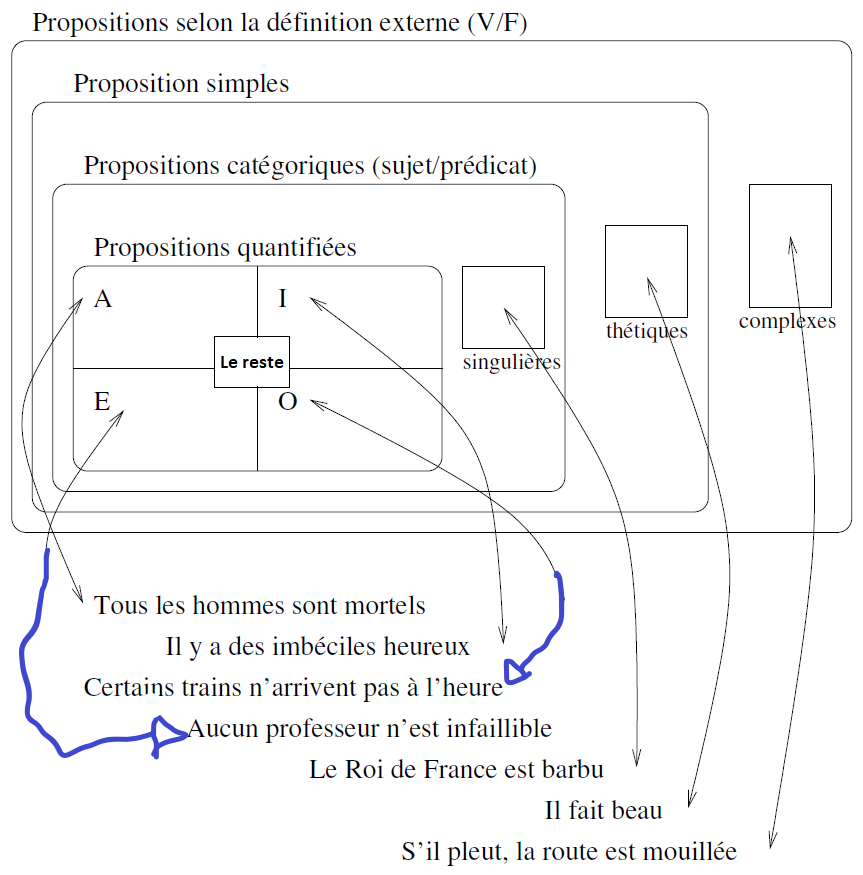
\includegraphics[scale=0.31]{syntheseProps.png}
\end{frame}




%---------------- intro -------------------

\begin{frame}
	\titre{Relations entre propositions}

			\begin{description}[labelindent=6pt,style=multiline,leftmargin=1.3in]
		 \setlength\itemsep{1em}
\item[Inverse \only<5->{?}] \textcolor{white}{lol} 
	 \pause
\item[Exemple] Tout prof est sympa\pause 
\item[] Quelle est la proposition \textit{inverse} ?\pause 
\item[] `Aucun prof n'est sympa` ?\pause 
\item[] Ca dépend de ce qu'on appelle l'\textit{inverse}\pause
\item[] On va distinguer les notions de propositions \textbf{contraires} et \textbf{contradictoires}
	\end{description}
	
\end{frame}



%------------------ Contraire ----------------------
\begin{frame}
	\titre{Relations entre propositions}

			\begin{description}[labelindent=6pt,style=multiline,leftmargin=1.3in]
		 \setlength\itemsep{1em}
\item[Contraires] P et Q sont contraires $\equiv$ elles ne peuvent pas être vraies en même temps 
	 \pause
%\item[En maths] $(P \rightarrow \neg Q) \wedge (Q \rightarrow \neg P)$\pause 
\item[En français] P et Q sont incompatibles\pause 
\item[Exemple] Proposition contraire de `Tout prof est sympa` ?\pause 
\item[] `Aucun prof n'est sympa` ? \pause Oui\pause
\item[] On peut en trouver d'autres ?\pause
\item[] `Il y a au moins un prof qui n'est pas sympa`
	\end{description}
\end{frame}



\begin{frame}
	\titre{Relations entre propositions}

			\begin{description}[labelindent=6pt,style=multiline,leftmargin=1.3in]
		 \setlength\itemsep{1em}
\item[Contraires] P et Q sont incompatibles
	 \pause
%\item[En maths] $(P \rightarrow \neg Q) \wedge (Q \rightarrow \neg P)$\pause 
\item[Exemple] Propositions contraires de `Le chat est mort et le chien est blond` ?\pause 
\item[] Le chat n'est pas mort \pause 
\item[] Le chien n'est pas blond\pause
\item[] Le chat n'est pas mort et le chien n'est pas blond\pause
\item[] Le chat n'est pas mort ou le chien n'est pas blond
	\end{description}
\end{frame}




%------------------------ Contradiction ----------------------------

\begin{frame}
	\titre{Relations entre propositions}

			\begin{description}[labelindent=6pt,style=multiline,leftmargin=1.3in]
		 \setlength\itemsep{1em}
\item[Contradiction] P et Q sont contradictoires si et seulement si elles ne peuvent être ni vraies ni fausses en même temps 
	 \pause
%\item[En maths] $(P \rightarrow \neg Q) \wedge (Q \rightarrow \neg P)$\pause 
\item[En français] On a toujours soit P, soit Q\pause 
\item[Exemple] Proposition contradictoire de `Tout prof est sympa` ?\pause 
\item[] `Il y a au moins un prof qui n'est pas sympa`\pause
\item[] Une autre ? \pause Non, pour toute proposition P, \textbf{unicité} de $\neg P$ (à reformulation près)
	\end{description}
\end{frame}



\begin{frame}
	\titre{Relations entre propositions}

			\begin{description}[labelindent=6pt,style=multiline,leftmargin=1.3in]
		 \setlength\itemsep{1em}
\item[Contradiction] On a toujours soit P, soit Q
	 \pause
%\item[En maths] $(P \rightarrow \neg Q) \wedge (Q \rightarrow \neg P)$\pause 
\item[Exemple] Le chat est mort et le chien est blond\pause 
\item[$\neg$] Le chat n'est pas mort ou le chien n'est pas blond\pause 
\item[Exemple] Certaines baleines sont sympathiques\pause
\item[$\neg$] Aucune baleine est sympathique \pause
\item[Exemple] Certains films français sont pas géniaux \pause
\item[$\neg$] Tous les films français sont géniaux 
	\end{description}
\end{frame}


\begin{frame}
	\titre{Relations entre propositions}

			\begin{description}[labelindent=6pt,style=multiline,leftmargin=1.3in]
		 \setlength\itemsep{1em}
\item[Contradiction] On a toujours soit P, soit Q
	 \pause
%\item[En maths] $(P \rightarrow \neg Q) \wedge (Q \rightarrow \neg P)$\pause 
\item[Exemple] Personne ne comprend ce cours \pause
\item[$\neg$] Quelqu'un comprend ce cours\pause
\item[Question] Vous avez remarqué quelque chose ?\pause
\item[] Quelque chose qui ressemblerait à une règle concernant les contradictions et les propositions quantifiées ?
	\end{description}
\end{frame}


\begin{frame}
	\titre{Relations entre propositions}

			\begin{description}[labelindent=6pt,style=multiline,leftmargin=1.3in]
		 \setlength\itemsep{1em}
\item[A] Tous les profs sont gentils
	 \pause
%\item[En maths] $(P \rightarrow \neg Q) \wedge (Q \rightarrow \neg P)$\pause 
\item[I] Quelques profs sont gentils\pause
\item[E] Aucun prof n'est gentil \pause
\item[O] Quelques profs ne sont pas gentils\pause
\item[Question] Que peut-on dire de chaque couple tiré dans cette liste de propositions ?\pause
\item[Indice] On va devoir introduire deux nouvelles relations (simples) entre propositions
	\end{description}
\end{frame}


\begin{frame}
	\titre{Le carré d'opposition}
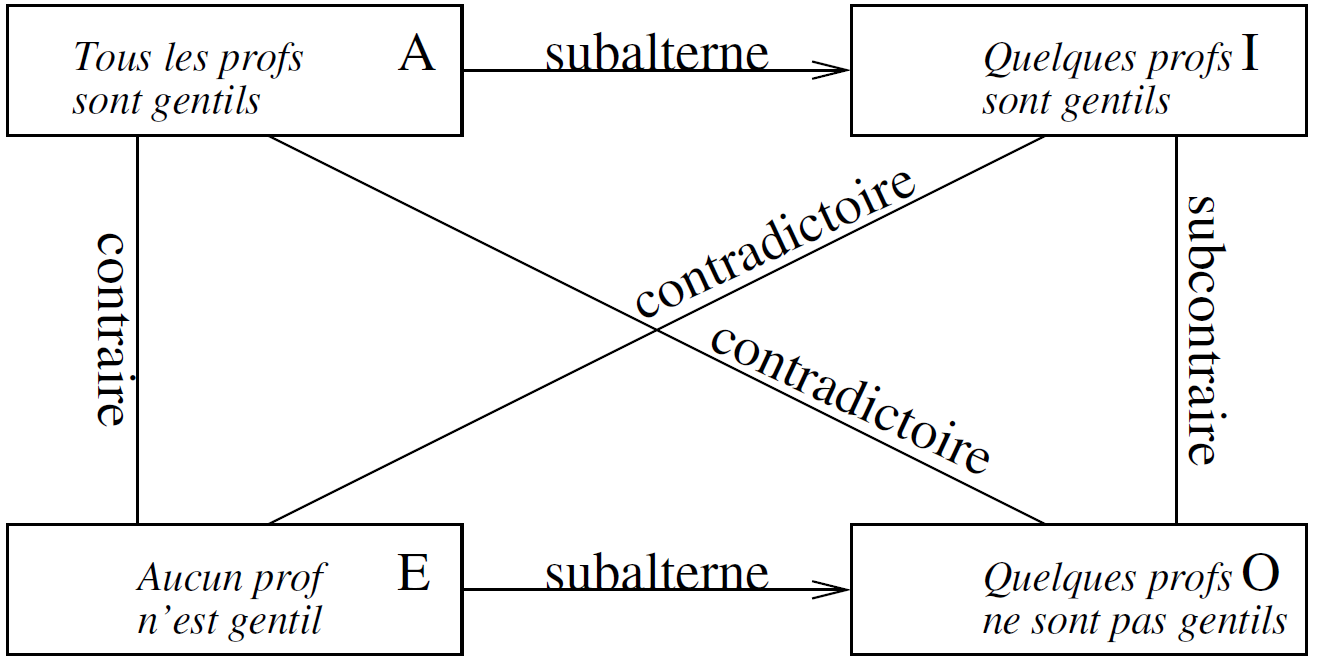
\includegraphics[scale=0.32]{carre.png}
\end{frame}


\begin{frame}
	\titre{Le carré d'opposition}

			\begin{description}[labelindent=6pt,style=multiline,leftmargin=1.3in]
		 \setlength\itemsep{1em}
\item[Subcontraire] P et Q sont subcontraires si elle ne peuvent pas être fausses en même temps\pause
\item[Remarque] I et O sont subcontraires, tandis que leurs contradictions (ou négations) sont contraires entre elles\pause
\item[] Coïncidence ? \pause Sans doute pas\pause
\item[Subalterne] P est subalterne de Q si Q implique P\pause, c'est à dire si chaque fois que Q est vraie, P l'est nécessairement aussi.
	 \pause
\item[def alternative] P est une version appauvrie (en information) de Q
	\end{description}
\end{frame}


\begin{frame}
	\titre{Le début du merdier}
			\begin{description}[labelindent=6pt,style=multiline,leftmargin=1.3in]
		 \setlength\itemsep{1em}
\item[Contraires] P et Q sont contraires $\equiv$ elles ne peuvent pas être vraies en même temps 
\item[Contradiction] On a toujours soit P, soit Q\pause
\item[Cependant] Pour les logiciens ... \pause c'est le contraire !\pause
\item[] Ils ont néanmoins plus l'habitude de dire `propositions inverses` que contraires \pause
\item[] On utilisera $P = \neg Q$ pour `soit P, soit Q` et `P X Q` pour `pas en même temps`
\item[Attention] `P X Q` pas canonique !
	\end{description}
\end{frame}



\begin{frame}
	\titre{Un autre carré bonus}
	
	DM !
%			\begin{description}[labelindent=6pt,style=multiline,leftmargin=1.3in]
%		 \setlength\itemsep{1em}
%\item[Remarque] On dira `R implique S` plutôt que `S est subalterne de R` (vieillot)\pause
%\item[Faits] (P et Q) implique P
%\item[] (P et Q) implique Q\pause
%\item[Explication] On passe de deux infos à une seule d'entre elles, on peut donc parler de perte d'information 
	%\end{description}
\end{frame}

%\begin{frame}
%	\titre{Un autre carré bonus}
%			\begin{description}[labelindent=6pt,style=multiline,leftmargin=1.3in]
%		 \setlength\itemsep{1em}
%\item[Faits] P implique (P ou Q)
%\item[] Q implique (P ou Q)\pause
%\item[Explication] Ici c'est plus fin, mais le même phénomène apparaît : on \textit{brouille} une information autrefois sûre avec une alternative potentielle\pause
%\item[Remarque] On obtient un carré qui permet d'expliquer au sein de la logique comment le `ou` logique inclusif devient exclusif en pratique (cf l'explication en cours)
%	\end{description}
%\end{frame}
%
%


	
\begin{frame}
	\titre{Intro à Port-Royal}
	
	\begin{description}[labelindent=6pt,style=multiline,leftmargin=1.3in]
		 \setlength\itemsep{1.4em}
		 
		 \item[Qui] Antoine Arnauld et Pierre Nicole
		 \pause
		 \item[Où] L'abbaye de Port-Royal (rien à voir avec le métro), haut lieu du jansénisme à l'époque
		 \pause
		 \item[Quand] 1662
		 \pause
		 \item[Quoi] Le bouquin `La logique ou l'art de penser`
		 
	\end{description}
\end{frame}



\begin{frame}
	\titre{Intro à Port-Royal}
	
	\begin{description}[labelindent=6pt,style=multiline,leftmargin=1.3in]
		 \setlength\itemsep{1.4em}
		 
		 \item[But] Distinguer les bons des mauvais syllogismes
		 \pause
		 \item[] C'est à dire ceux qui sont \textbf{valides} et ceux qui ne le sont pas
		 \pause
		 \item[Problème] Y a du travail
		 \pause
		 \item[`Solution`] \textit{Fixer avec précision l'objet d'étude} \pause (cad se resteindre à un chantier plus simple) \pause
		 \item On s'intéresse uniquement aux raisonnements avec 2 prémisses + 1 conclusion\pause, le tout quantifié
 		 
	\end{description}
\end{frame}



\begin{frame}
	\titre{Intro à Port-Royal}
	
	\begin{description}[labelindent=6pt,style=multiline,leftmargin=1.3in]
		 \setlength\itemsep{1em}
		 
		 \item[Rappel] Les \textit{termes} utilisés dans un raisonnement n'ont pas (vraiment) d'importance
		 \pause
		 \item[] \begin{tabular}{l}
Tous les alcooliques sont bigleux\\
Tous les bigleux sont blonds\\ \cline{1-1}
Tous les alcooliques sont blonds\\
\end{tabular}
		 \item[$\equiv$] \begin{tabular}{l}
Tous les barmans sont chauves\\
Tous les chauves sont méchants\\ \cline{1-1}
Tous les barmans sont méchants\\
\end{tabular}\pause


		 \item[$\equiv$] \begin{tabular}{l}
Tous les X sont Y\\
Tous les Y sont Z\\ \cline{1-1}
Tous les X sont Z\\
\end{tabular}
	\end{description}
\end{frame}


\begin{frame}
	\titre{Intro à Port-Royal}
	
	\begin{description}[labelindent=6pt,style=multiline,leftmargin=1.3in]
		 \setlength\itemsep{1em}
		 
		 \item[Idée] On peut donc espérer \textit{énumérer} (lister) l'ensemble des \textbf{schémas} possibles si on trouve les \textbf{paramètres} pertinents
		 \pause
		 \item[Définition] Les conclusions seront de la forme 
\begin{tabular}[t]{clc}
B &est& A\\
\textbf{petit terme} &&\textbf{grand terme}\\
\end{tabular}
 \pause
		 \item[Définition] Pour répondre à la question, on va passer par un autre terme, le \textbf{moyen}
\pause

		 \item[]
\begin{tabular}{cccl}
A  & $\leftrightarrow$ & M & (prémisse) majeure\\
M  & $\leftrightarrow$ & B & (prémisse) mineure\\
\hline
B  & est & A & conclusion\\
\end{tabular}
	\end{description}
\end{frame}


\begin{frame}
	\titre{Figures}
	
	\begin{description}[labelindent=6pt,style=multiline,leftmargin=1.3in]
		 \setlength\itemsep{1em}
		 
		 \item[]
\begin{tabular}{cccl}
A  & $\leftrightarrow$ & M & (prémisse) majeure\\
M  & $\leftrightarrow$ & B & (prémisse) mineure\\
\hline
B  & est & A & conclusion\\
\end{tabular}

\item[Remarque] L'ordre peut changer (d'où les $\leftrightarrow$)\pause, pour un total de 4 combinaisons
\pause
\item[Constantes] A (grand terme) = attribut de la conclusion \pause
\item[] B (petit terme) = sujet de la conclusion \pause 
\item[] M (moyen) = attribut ou sujet \newline \pause 
	\end{description} 

	Majeure (resp. Mineure) = prémisse impliquant le grand (resp. petit) terme 
\end{frame}




\begin{frame}
	\titre{Figures}
	
	\begin{tabular}{ccc}
\begin{tabular}{lcc}
1\iere\ figure	& M & A \\
		& B & M \\
\cline{2-3}
		& B & A \\
\end{tabular}
%

&
\textcolor{white}{lolilol}
&
\begin{tabular}{lcc}
2\ieme\ figure	& A & M \\
		& B & M \\
\cline{2-3}
		& B & A \\
\end{tabular} \\
%


\textcolor{white}{lolilol} & 
\textcolor{white}{lolilol} & 
\textcolor{white}{lolilol} \\


\textcolor{white}{lolilol} & 
\textcolor{white}{lolilol} & 
\textcolor{white}{lolilol} \\


\textcolor{white}{lolilol} & 
\textcolor{white}{lolilol} & 
\textcolor{white}{lolilol} \\

\begin{tabular}{lcc}
3\ieme\ figure	& M & A \\
		& M & B \\
\cline{2-3}
		& B & A \\
\end{tabular}

&
\textcolor{white}{lolilol}
&
\begin{tabular}{lcc}
4\ieme\ figure	& A & M \\
		& M & B \\
\cline{2-3}
		& B & A \\
\end{tabular}
\end{tabular}
\end{frame}



\begin{frame}
	\titre{Modes}
	
	\begin{description}[labelindent=6pt,style=multiline,leftmargin=1.3in]
		 \setlength\itemsep{1em}

\item[Mode] Arrangement de 3 propositions ayant 4 formes possibles (A, I, E ou O) \pause $\rightarrow$ 64 combinaisons (AAA, EIO, AEE, etc ...)\pause
\item[] On va pouvoir combiner figure et mode \pause : si le mode est $Q_1Q_2Q_3$, la grand prémisse sera $Q_1$, la petite sera $Q_2$ et la conclusion sera $Q_3$. \pause
\item[But du jeu] Essayer toutes les figures avec tous les modes \pause pour un total de 256 syllogismes à tester ! 

	\end{description} 
\end{frame}



\begin{frame}
	\titre{C'est parti ! (1/256)}
	
	\begin{description}[labelindent=6pt,style=multiline,leftmargin=1.3in]
		 \setlength\itemsep{1em}

\item[$3^{\grave{e}me}$ figure] \begin{tabular}{cc}
M & A \\
	M & B \\
\cline{1-2}
		B & A \\
\end{tabular}
\item[Mode] AAA \pause
\item[Attention] Les `A` du mode et ceux de la figure n'ont rien à voir ! \pause (personne n'a dit que le formalisme était bien foutu) \pause
\item[Question] Valide ? 

	\end{description} 
\end{frame}



\begin{frame}
	\titre{C'est parti ! (1/256)}
	
	\begin{description}[labelindent=6pt,style=multiline,leftmargin=1.3in]
		 \setlength\itemsep{1em}

\item[Mode + figure] \begin{tabular}{c}
Tous les M sont A\\ 
Tous les M sont B\\ 
\cline{1-1}
Tous les B sont A
\end{tabular} \pause
\item[Explication] On peut imaginer un monde dans lequel il y a uniquement 2 individus, Jean-Michel qui est à la fois M, A et B, et Jean-Charles qui est uniquement B \pause
\item[] Les deux \textbf{hypothèses} sont \textbf{respectées} (tout M est également A et B), mais la \textbf{conclusion} est \textbf{fausse} (JC l'enfreint)\pause
\item[Réponse] Pas valide, car on a un \textbf{contre-exemple} 

	\end{description} 
\end{frame}


\begin{frame}
	\titre{C'est parti ! (1/256)}
	
	\begin{description}[labelindent=6pt,style=multiline,leftmargin=1.3in]
		 \setlength\itemsep{1em}

\item[Mode + figure] \begin{tabular}{c}
Tous les M sont A\\ 
Tous les M sont B\\ 
\cline{1-1}
Tous les B sont A
\end{tabular}
\item[Explication] On peut imaginer un monde dans lequel il y a uniquement 2 individus, Jean-Michel qui est à la fois M, A et B, et Jean-Charles qui est uniquement B
\item[Remarque] Un truc à dire sur ce contre-exemple \only<1>{? \textcolor{white}{pour l'améliorer}}\only<2->{pour l'améliorer ?}\pause  \pause
\item[] Il n'est pas minimal\pause, on peut se passer de Jean-Michel

	\end{description} 
\end{frame}



\begin{frame}
	\titre{Méthodologie}
	
	\begin{description}[labelindent=6pt,style=multiline,leftmargin=1.3in]
		 \setlength\itemsep{1em}
		 
\item[Remarque] \textbf{Un (contre-)exemple sert uniquement à montrer qu'un syllogisme n'est pas valide} \pause
\item[] On pourrait aussi imaginer un monde où il y a un seul individu, qui est M, A et B\pause
\item[] Dans ce cas, hypothèses + conclusion respectées\pause
\item[] Le syllogisme n'en est pas pour autant valide !
\item[] Pour montrer la validité, ça va donc être un peu plus abstrait 
	\end{description} 

	
\end{frame}

\begin{frame}
	\titre{Méthodologie}
	
	\begin{description}[labelindent=6pt,style=multiline,leftmargin=1.3in]
		 \setlength\itemsep{1em}
		 
\item[Par contre] Les contre-exemples se présentent très bien sous la forme de \textbf{diagrammes de Venn} (aussi appelés patatoïdes)\pause
\item[Exemple] 	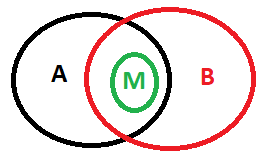
\includegraphics[scale=0.5]{1256.png}\pause
\item[] Chaque \textit{patate} représente l'ensemble des individus qui ont la propriété associée\pause
\item On a bien les hypothèses respectées et la conclusion falsifiée
	\end{description} 

	
\end{frame}







%
%\begin{frame}
%	\titre{C'est parti ! (1/256 prise 2)}
%	
%	\begin{description}[labelindent=6pt,style=multiline,leftmargin=1.3in]
%		 \setlength\itemsep{1em}
% 
%\item[Exemple] 
%\begin{tabular}{c}
%Tous les canards sont mexicains \\
%	Tous les canards jouent au poker \\
%\cline{1-1}
%Tous les joueurs de poker sont mexicains \\
%\end{tabular}
%\pause
%\item[Explication] Soit un monde dans lequel tous les canards sont des joueurs de poker mexicains, et Jean-Luc un joueur de poker non-canard, non-mexicain. Aucune des hypothèses n'est violée, tandis que la conclusion n'est pas vraie. \pause
%\item[Réponse] Pas valide, car on a un \textbf{contre-exemple} 
%	\end{description} 
%\end{frame}
%


\begin{frame}
	\titre{C'est parti ! (2/256)}
	
	\begin{description}[labelindent=6pt,style=multiline,leftmargin=1.3in]
		 \setlength\itemsep{1em}

\item[$1^{\grave{e}re}$ figure] \begin{tabular}{cc}
M & A \\
	B & M \\
\cline{1-2}
		B & A \\
\end{tabular}
\item[Mode] AAA \pause
\item[Question] Valide ? 

	\end{description} 
\end{frame}



\begin{frame}
	\titre{C'est parti ! (2/256)}
	
	\begin{description}[labelindent=6pt,style=multiline,leftmargin=1.3in]
		 \setlength\itemsep{1em}

\item[Mode + figure] \begin{tabular}{c}
Tous les M sont A\\ 
Tous les B sont M\\ 
\cline{1-1}
Tous les B sont A
\end{tabular} \newline
	\end{description}
	
Prenons un B \textbf{arbitraire}\pause, cad sur lequel on n'a aucune autre information \pause
\newline 

La prémisse min. nous dit qu'il est aussi M\pause
\newline

La prémisse maj. nous dit alors qu'il est aussi A\pause \newline

Syllogisme valide \pause : on a montré qu'un individu, \textbf{dont on savait seulement qu'il était B}, est aussi un A. \pause Ca prouve que \textbf{n'importe quel B} sera aussi A

\end{frame}


\begin{frame}
	\titre{C'est parti ! (2/256 prise 2)}
	
	\begin{description}[labelindent=6pt,style=multiline,leftmargin=1.3in]
		 \setlength\itemsep{1em}

\item[Mode + figure] \begin{tabular}{c}
Tous les M sont A\\ 
Tous les B sont M\\ 
\cline{1-1}
Tous les B sont A
\end{tabular} \newline
	\end{description}
	
	 
Prenons un B \textbf{arbitraire}, cad sur lequel on n'a aucune autre information \pause \newline 

La prémisse min. permet de le \textbf{transformer} en M\pause \newline

La prémisse maj. permet de \textbf{transformer} le M obtenu en A \pause \newline

Syllogisme valide \pause : on a montré qu'en \textbf{composant} (combinant) les deux prémisses, on crée \only<1-4>{\textcolor{white}{une \textit{méthode}}}\only<5>{une \textit{méthode}}\only<6>{une \textit{fonction}}\only<7>{un \textbf{programme}} permettant de \textbf{transformer} tout B en A \pause

\end{frame}


%
%\begin{frame}
%	\titre{Méthodo validité}
%	
%Dans le cas d'une démonstration de non-validité d'un syllogisme, vous pouvez utiliser des exemples `concrets` ou rester abstrait, selon ce avec quoi vous êtes le plus à l'aise \newline
%\pause
%
%La non-importance des termes fait que vous pourriez théoriquement avoir le même choix au moment de prouver la validité d'un syllogisme\pause, mais pour vous faire prendre des bonnes habitudes, on va se limiter à l'abstrait \newline
%
%\pause
%En maths, un \textbf{exemple} ne prouve pas un résultat \textit{général}. Ici c'est un cas un peu dégénéré qu'on va donc ignorer.
%
%\end{frame}


\begin{frame}
	\titre{La slide barbante}
	
Vous pouvez choisir d'utiliser le style `$x$ est un A et telle prémisse nous dit que tout A est aussi un M, donc $x$ est un M`\pause, ou `x est un A et telle prémisse permet de \textit{transformer} tout A en M, donc on peut faire de x un M`. \newline \pause

La différence n'est sans doute pas évidente, mais représente les deux (grosses) approches des fondements des mathématiques ! \pause \newline

Le premier style correspond à un point de vue \textbf{théorie des ensembles} (patatoïdes), tandis que la deuxième formulation découle de la \textbf{théorie des types} (programmes). \pause Le schisme entre ces deux théories est une conséquence du \textbf{paradoxe de Russel} (1901$\sim$1903).

\end{frame}



\begin{frame}
	\titre{C'est (re-)parti ! (3/256)}
	
	\begin{description}[labelindent=6pt,style=multiline,leftmargin=1.3in]
		 \setlength\itemsep{1em}

\item[$2^{\grave{e}me}$ figure] \begin{tabular}{cc}
A & M \\
	B & M \\
\cline{1-2}
		B & A \\
\end{tabular}
\item[Mode] AAI \pause
\item[Question] Valide ? 

	\end{description} 
\end{frame}



\begin{frame}
	\titre{C'est (re-)parti ! (3/256)}
	
	\begin{description}[labelindent=6pt,style=multiline,leftmargin=1.3in]
		 \setlength\itemsep{1em}

\item[Mode + figure] \begin{tabular}{c}
Tous les A sont M\\ 
Tous les B sont M\\ 
\cline{1-1}
Certains B sont A
\end{tabular}\pause
\item[Explication] On peut imaginer un monde dans lequel il y a seulement 2 individus : Jean-Michel qui est à la fois A et M, et Jean-Charles qui est uniquement B et M\pause
\item[] Les deux hypothèses sont respectées (tout individu A ou B est également M), mais la conclusion est fausse (le seul B n'est pas A)\pause
\item[Réponse] Pas valide, car on a un \textbf{contre-exemple} 

	\end{description} 
\end{frame}


\begin{frame}
	\titre{C'est (re-)parti ! (3/256 bonus)}
	
	\begin{description}[labelindent=6pt,style=multiline,leftmargin=1.3in]
		 \setlength\itemsep{1em}

\item[AAX + fig. 3] \begin{tabular}{c}
Tous les A sont M\\ 
Tous les B sont M\\ 
\cline{1-1}
[relation entre A et B]
\end{tabular} \pause
\item[Remarque] Etant donnée la figure, aucun mode de la forme AAX ne sera valide
\pause
\item[] En effet, imaginez que M est l'ensemble des individus\pause, alors les deux prémisses deviennent `tous les individus ayant la prop A (ou B) sont des individus`\pause
\item[] Ca n'apporte strictement aucune information, on ne va rien pouvoir conclure

	\end{description} 
\end{frame}






\begin{frame}
	\titre{C'est (re-)parti ! (7/256)}
	
	\begin{description}[labelindent=6pt,style=multiline,leftmargin=1.3in]
		 \setlength\itemsep{1em}

\item[$1^{\grave{e}re}$ figure] \begin{tabular}{cc}
M & A \\
	B & M \\
\cline{1-2}
		B & A \\
\end{tabular}
\item[Mode] III \pause
\item[Question] Valide ? 

	\end{description} 
\end{frame}



\begin{frame}
	\titre{C'est (re-)parti ! (7/256)}
	
	\begin{description}[labelindent=6pt,style=multiline,leftmargin=1.3in]
		 \setlength\itemsep{1em}

\item[Mode + figure] \begin{tabular}{c}
Certains M sont A\\ 
Certains B sont M\\ 
\cline{1-1}
Certains B sont A
\end{tabular}\pause
\end{description}
\only<1>{\vspace{5cm}}
\only<2-3>{
	\begin{description}[labelindent=6pt,style=multiline,leftmargin=1.3in]
		 \setlength\itemsep{1em}
\item[Contre-ex] On a 10 individus $p_1$ à $p_{10}$. $p_1$ est M et A (et pas B), $p_2$ est B et M (et pas A), le reste n'est jamais A et B à la fois\pause
\item[] Les deux hypothèses sont respectées (grâce à $p_1$ et $p_2$), mais la conclusion est fausse (peut se vérifier sur chaque individu)\pause
\end{description}
\vspace{1.47cm}
}

\only<4>{
	\vspace{1.2cm}
	\begin{figure}[H]
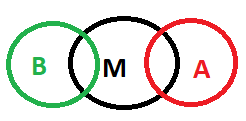
\includegraphics[scale=0.5]{4256.png}
\end{figure}\vspace{1.9cm}}

\pause

\only<5>{
	\vspace{1.2cm}
	\begin{figure}[H]
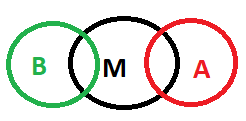
\includegraphics[scale=0.5]{4256.png}
\end{figure}
	\begin{description}[labelindent=6pt,style=multiline,leftmargin=1.3in]
		 \setlength\itemsep{1em}
\item[Réponse] Pas valide, car on a un \textbf{contre-exemple} 
	\vspace{1.1cm}
	\end{description}}

	 
\end{frame}



\begin{frame}
	\titre{C'est (re-)parti ! (7/256)}
	
	\begin{description}[labelindent=6pt,style=multiline,leftmargin=1.3in]
		 \setlength\itemsep{1em}

\item[Mode + figure] \begin{tabular}{c}
Certains M sont A\\ 
Certains B sont M\\ 
\cline{1-1}
Certains B sont A
\end{tabular}
	\end{description} 
De façon générale, on ne pourra jamais rien tirer de deux propositions particulières\pause \newline

Quel que soit le type (A / E / I / O) de la conclusion, on pourra créer une situation qui valide les deux hypotheses (particulières) sans valider la conclusion (comme on vient de le faire)\pause \newline

En fait, pas mal de règles de ce type, qui réduisent l'ensemble des syllogisme à tester, ont été identifiées.


\end{frame}
	


\begin{frame}
	\titre{Règles de base des syllogismes}
	
	\begin{itemize}
	
	\item[1] Le moyen doit être pris au moins une fois universellement\pause
	\item[2]   Les termes de la conclusion ne peuvent point être pris plus universellement dans la conclusion que dans les prémisses\pause
	\item[3]  On ne peut rien conclure de deux propositions négatives\pause
	\item[4]  On ne peut prouver une conclusion négative par deux propositions affirmatives\pause
	\item[5]  La conclusion suit toujours la plus faible partie, cad que s'il y a une des deux propositions négatives, elle est négative, et s'il y en a une particulière, elle doit être particulière\pause
	\item[6]  De deux propositions particulières il ne s'ensuit rien
	
	\end{itemize}
	
\end{frame}
	


\begin{frame}
	\titre{Pause discussion}
	
	\begin{description}[labelindent=6pt,style=multiline,leftmargin=1.3in]
		 \setlength\itemsep{1em}

\item[Remarques] ?\pause
\item[Pts positifs] Différence vérité / validité\pause
\item[] Début de classification ...\pause
\item[Pts négatifs] ... un peu bancale ...\pause
\item[] ... et arbitraire\pause
\item[] Système très \textbf{incomplet} (les propositions valides ne sont pas toutes couvertes) ... \pause
\item[] ... et pourtant redondant (cf A / E / I / O)
\end{description}
\end{frame}
	
	

% 6/256

\begin{frame}
	\titre{C'est (re-)parti ! (?/256)}
	
	\begin{description}[labelindent=6pt,style=multiline,leftmargin=1.3in]
		 \setlength\itemsep{1em}

\item[$4^{\grave{e}me}$ figure] \begin{tabular}{ll}
A & M \\
	M & B \\
\cline{1-2}
		B & A \\
\end{tabular}
\item[Mode] EAO \pause
\item[Question] Valide ? 

	\end{description} 
\end{frame}



\begin{frame}
	\titre{C'est (re-)parti ! (?/256)}
	
	\begin{description}[labelindent=6pt,style=multiline,leftmargin=1.3in]
		 \setlength\itemsep{1em}

\item[Mode + figure] \begin{tabular}{l}
Aucun A n'est M\\ 
Tous les M sont B\\ 
\cline{1-1}
Certains B ne sont pas A
\end{tabular} \newline
	\end{description} \pause
Quand on a une conclusion négative, c'est souvent plus simple de raisonner par l'absurde\pause \newline

On part du principe (potentiellement abusivement ...) que toute propriété est soit fausse, soit vraie.\newline \pause

Si on prouve qu'elle ne peut pas être fausse, elle doit donc forcément être vraie. \pause On va donc supposer qu'elle est fausse, et voir si ça introduit un paradoxe, auquel cas on a gagné.
\end{frame}


\begin{frame}
	\titre{C'est (re-)parti ! (?/256)}
	
	\begin{tabular}{l}
\textcolor{green}{Aucun A n'est M}\\ 
\textcolor{red}{Tous les M sont B}\\ 
\textcolor{blue}{Tous les B sont A}\\ 
\cline{1-1}
[Paradoxe, fin du monde, invasion de sauterelles] \\
\textcolor{white}{lol}
\end{tabular} \newline \pause

\begin{tabular}{cc}
\begin{tabular}{l}
\textcolor{red}{Tous les M sont B}\\ 
\textcolor{blue}{Tous les B sont A}\\ 
\cline{1-1}
\textcolor{purple}{Tous les M sont A}\\
\textcolor{white}{lol}
\end{tabular} 
& \pause \begin{tabular}{l}
\textcolor{purple}{Tous les M sont A}\\
\textcolor{green}{Aucun A n'est M}\\ 
\cline{1-1}
[Paradoxe]\\
\textcolor{white}{lol}
\end{tabular}\end{tabular}\pause
	
En acceptant les deux prémisses originales, `Tous les B sont A` impossible\pause, donc la négation (contradiction) est vraie\pause \newline

On a donc bien `Certains B ne sont pas A`\pause, n'est-ce pas ?

\end{frame}


\begin{frame}
	\titre{Twist}
En fait non, on peut créer un contre-exemple !\pause \newline

Soit un monde dans lequel personne n'est M et où tous les B sont A (puisque c'est un contre-exemple, on choisit)\newline\pause

`Aucun A n'est M` $\Rightarrow$ c'est automatiquement vrai\pause \newline

`Tous les M sont B` $\Rightarrow$ c'est plus étrange, mais c'est vrai aussi : il est vrai que \textbf{chaque} M est aussi un B\pause \newline

 La conclusion `certains B ne sont pas A` est quant à elle fausse. C'est donc bien un contre-exemple

\end{frame}


\begin{frame}
	\titre{Twist}
	
	\begin{description}[labelindent=6pt,style=multiline,leftmargin=1.3in]
		 \setlength\itemsep{1em}
		 \item[Euh, ok ?] Pourquoi ce détour apparemment inutile ?\pause
		 \item[] Étonnement, c'est une `configuration` ($4^{\grave{e}me}$ figure, mode EAO) qui jugée valide dans Port-Royal
		 \end{description}

 \pause	 
	\begin{description}[labelindent=6pt,style=multiline,leftmargin=1.3in]
		 \setlength\itemsep{1em}
		 \item[Alors quoi ?] Une \underline{piste} intéressante à étudier, c'est la notion de \textbf{vérité}
		 %\item[Attention] On étudie la \textbf{validité} des syllogismes, mais la définition utilise celle de la vérité
 	\end{description}
\end{frame}


\begin{frame}
	\titre{Twist}
	
	\begin{description}[labelindent=6pt,style=multiline,leftmargin=1.3in]
		 \setlength\itemsep{1em}
		 \item[Attention] On étudie la \textbf{validité} des syllogismes, mais la définition utilise celle de la vérité\pause
		 \item[] `Dans un monde où les prémisses sont \textbf{vraies}, est-ce qu'on peut assurer que la conclusion sera \textbf{vraie} aussi ? `\pause
		 \item[Question] Dans un monde où personne n'est M, dans quelle mesure est-il vrai que `tous les M sont B` et que `aucun A n'est M` ?\pause
		 \item[Réponse] \textit{Techniquement} c'est vrai, mais \textit{en pratique}, c'est très étrange. \pause Distinction \textbf{sémantique} / \textbf{pragmatique}
 	\end{description}
\end{frame}




\begin{frame}
	\titre{Twist}
	
	\begin{description}[labelindent=6pt,style=multiline,leftmargin=1.3in]
		 \setlength\itemsep{1em}
		 \item[Sémantique] Construction du sens \textit{strict}\pause
		 \item[Pragmatique] Le sens \textit{en pratique}\pause
		 \item[Exemples] Comment le [ou inclusif] logique devient en pratique le [ou exclusif] en pratique \pause
		 \item[] Utilisation de `moins de [un nombre]` \pause
		 \item[] `aucun A n'est M` qui ne passe pas dans un monde où rien n'est M\pause
		 \item[] La linguistique moderne fait bien la distinction entre sémantique et pragmatique, PR non
		 
 	\end{description}
\end{frame}



\begin{frame}
	\titre{Au final}
	
	Liste des syllogismes jugés valides par Port-Royal :
	
	\begin{tabular}{cccc}
	\textcolor{white}{lol} & \textcolor{white}{lol} & \textcolor{white}{lol} & \textcolor{white}{lol} \\
\rm 1\iere\ figure & \rm 2\ieme\ figure & \rm 3\ieme\ figure & \rm 4\ieme\ figure\\
\hline
AAA&AOO&\color{black}AAI&\color{black}AAI\\
\color{black}AII&\color{black}AEE&\color{black}AII&\color{black}AEE\\
\color{black}EAE&\color{black}EAE&\color{black}EAO&\color{black}EAO\\
EIO&EIO&EIO&EIO\\
   &   &\color{black}IAI&\color{black}IAI\\
   &   &OAO&   \\
\end{tabular}


	
\end{frame}





 \begin{frame}
 \titre{Conclusion}
 
 Bon, la logique de Port-Royal c'est pas exactement la formalisation ultime et absolue du raisonnement. \newline \pause
 
Certaines corrections ont été tentées, notamment par Leibniz. \pause Il introduit syllogismes supplémentaires (24 au lieu des 19 de PR), mais les problèmes du formalisme sont trop \textit{profonds}. \pause  \newline

Il introduit aussi des méthodes de \textit{calcul} (preuve) graphiques (patatoïdes (ou diagrammes de Venn), droites de Leibniz), mais rien de très satisfaisant.\pause \newline

Y a quand même des bonnes idées, qu'on va essayer de retrouver sur une base plus solide \pause : \textbf{la logique formelle !}
 
 \end{frame}
 
 
 
 
 
\begin{frame}
	\titre{Exercices - classification}

Diane est cool : \pause proposition singulière (on parle d'une personne clairement identifiée)\pause\newline

Les amis de Diane sont cool : \pause proposition universelle affirmative A (`tout individu ayant la propriété d'être un ami de Diane a aussi la propriété d'être cool`)\pause\newline

Diane et Elsa sont cool : \pause proposition complexe (composée de `Diane est cool` + `Elsa est cool`)\pause\newline

Au moins un ami de Diane n'est pas cool : \pause proposition particulière négative O (Il existe un individu qui a la propriété d'être un ami de Diane mais pas celle d'être cool)

\end{frame}
\begin{frame}
	\titre{Exercices - classification}

Un ami de Diane est cool : \pause proposition particulière affirmative I (Il existe un individu qui a la propriété d'être un ami et celle d'être cool) \pause ... ou universelle affirmative A !\newline\pause

Aucun ami de Diane n'est cool : \pause proposition universelle négative E (Tout individu ayant la propriété d'être un ami de Diane a la propriété de ne pas être cool)\pause\newline

Certains amis de Diane sont cool : \pause proposition particulière affirmative I

\end{frame}
\begin{frame}
	\titre{Exercices - classification}

L'ami pas cool de Diane est moche : \pause proposition singulière \pause (le `le` (abrégé en `l'`) présuppose que la personne mentionnée est clairement identifiée, c'est comme si on utilisait son nom)\pause\newline

Un ami moche de Diane est un bon ami : \pause proposition particulière affirmative I \pause ... ou universelle affirmative A
\end{frame}


\begin{frame}
	\titre{Exercices - négation}

$\neg$(Diane est cool) = \pause Diane n'est pas cool \pause ($\neg$(x est Y) = x n'est pas Y)\pause\newline

$\neg$(Les amis de Diane sont cool) = \pause Au moins un ami de Diane n'est pas cool\pause\newline

$\neg$(Diane et Elsa sont cool) = \pause Diane n'est pas cool ou Elsa n'est pas cool \pause ($\neg (P $ ET $ Q) = \neg P $ OU $ \neg Q$)\pause\newline

$\neg$(Au moins un ami de Diane n'est pas cool) = \pause Tous les amis de Diane sont cool

\end{frame}

\begin{frame}
	\titre{Exercices - négations}
	
	
$\neg$(Un ami de Diane est cool) = \pause Aucun ami de Diane n'est cool (si vous avez répondu I avant) ou Au moins un ami de Diane n'est pas cool (si A)\pause\newline


$\neg$(Aucun ami de Diane n'est cool) = \pause Au moins un ami de Diane est cool\pause\newline

$\neg$(Certains amis de Diane sont cool) = \pause Aucun ami de Diane n'est cool

\end{frame}
\begin{frame}
	\titre{Exercices - négations}
	
	
$\neg$(L'ami pas cool de Diane est moche) = \pause L'ami pas cool de Diane n'est pas moche\pause\newline

$\neg$(Un ami moche de Diane est un bon ami) = \pause Aucun ami de Diane n'est un bon ami (si I), ou Au moins un ami moche de Diane n'est pas un bon ami (si A)

\end{frame}




\begin{frame}
	\titre{Exercices - implications}

`Les amis de Diane sont cool` \appearsAt{2}{black}{$\rightarrow$} `Certains amis de Diane sont cool`\pause\pause\newline

`Aucun ami de Diane n'est cool` \appearsAt{4}{black}{$\rightarrow$} `Au moins un ami de Diane n'est pas cool`\pause\pause\newline

`Diane est cool` \appearsAt{6}{black}{$\leftarrow$} `Diane et Elsa sont cool`\pause\pause\newline

`L'ami pas cool de Diane est moche` \appearsAt{8}{black}{$\rightarrow$} `Au moins un ami de Diane n'est pas cool`\pause\pause\newline

`Certains amis de Diane sont cool`\appearsAt{10}{black}{$\not\leftrightarrow$} `Au moins un ami de Diane n'est pas cool` ! 	
\end{frame}


\begin{frame}
	\titre{Exercices - schémas}

\begin{tabular}{lc}
1$^{er}$ syllogisme & Tous les M sont A \\
		& Tous les B sont M \\
\cline{2-2}
		& Aucun B n'est A \\
\end{tabular}
\pause

Pas valide : \pause\newline
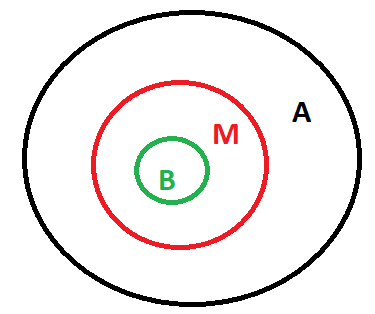
\includegraphics[scale=0.5]{S1DM3.png}

\end{frame}


\begin{frame}
	\titre{Exercices - schémas}

\begin{tabular}{lc}
2$^{\grave{e}me}$ syllogisme & Certains M sont A \\
		& Certains B ne sont pas M \\
\cline{2-2}
		& Certains B ne sont pas A \\
\end{tabular}
\pause

Pas valide : \pause\newline
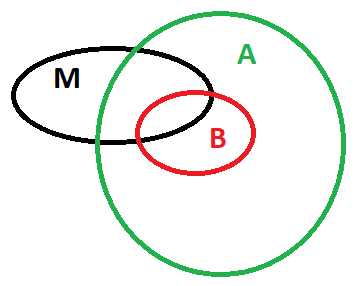
\includegraphics[scale=0.5]{S2DM3.png}

\end{frame}


\begin{frame}
	\titre{Exercices - schémas}

\begin{tabular}{lc}
3$^{\grave{e}me}$ syllogisme & Aucun M n'est A \\
		& Certains B sont M \\
\cline{2-2}
		& Certains B ne sont pas A \\
\end{tabular}
\pause
\textcolor{white}{lol}\newline

Valide : \pause La deuxième prémisse nous dit qu'il existe un individu qui est B et M, qu'on appellera $x$. \pause\newline

Or, la première prémisse nous dit que A et M sont des propriétés incompatibles. $x$, qui est déjà M, ne peut donc pas être A.\pause\newline

On a donc bien un individu, $x$, qui est B mais pas A
\end{frame}


\begin{frame}
	\titre{Exercices - schémas}

\begin{tabular}{lc}
4$^{\grave{e}me}$ syllogisme & Certains M sont A \\
		& Tous les B sont M \\
\cline{2-2}
		& Certains B ne sont pas A \\
\end{tabular}
\pause

Pas valide : \pause\newline
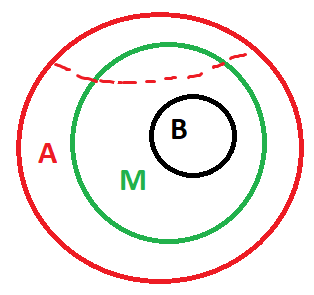
\includegraphics[scale=0.5]{S4DM3.png}

\end{frame}


%	
% \begin{frame}
% \titre{Rappels sur les propositions}
% 
% En linguistique, on dit que P et Q sont \textbf{contradictoires} ssi P et Q ne peuvent être ni vraies, ni fausses en même temps\pause, cad qu'il y en a toujours \textbf{exactement} une des deux qui est vraie\pause\newline
% 	
%Les logiciens, eux, disent que Q est la négation de P (ou l'inverse), et le notent $P \leftrightarrow \neg Q$. \pause On notera parfois (et de plus en plus) $\neg P$ (ou non-P) la proposition contradictoire / négation de P\pause\newline
%
%`non-(Takashi Miike est un réalisateur)` $\equiv$ \pause `Takashi Miike n'est pas réalisateur`\pause\newline
%
%`non-(Takashi Miike est un réalisateur japonais)` $\equiv$ \pause `Takashi Miike n'est pas réalisateur \underline{\textbf{ou}} n'est pas japonais`
% 
% \end{frame}
% 
% 
%\begin{frame}
%	\titre{Rappels sur les propositions}
%	
%
%`non-(P ou Q)` $\equiv$ \pause `(non-P et non-Q)`\newline\pause
%`non-(P et Q)` $\equiv$ \pause`(non-P ou non-Q)` \newline \pause
%
%\textcolor{white}{lalaaa}`non-((P ou Q) et (R ou S))` \newline$\equiv$ \textcolor{white}{lalal}\pause`non-(P ou Q) ou non-(R ou S)` \pause\newline
%$\equiv$ `(non-P et non-Q) ou (non-R et non-S)`\pause \newline
%
%
%\textcolor{white}{lalaaaa}`non-((P et Q) ou (R et S))` \newline$\equiv$ \textcolor{white}{lalaal}\pause`non-(P et Q) et non-(R et S)` \pause\newline
%$\equiv$ `(non-P ou non-Q) et (non-R ou non-S)` \pause \newline
%
%\end{frame}
%
%
%\begin{frame}
%	\titre{Rappels sur les propositions}
%	
%En linguistique, P et Q sont contraires ssi elles ne peuvent pas être vraies en même temps (elles sont incompatibles)\pause\newline
%
%En logique, il n'y a pas - à ma connaissance - de mot ou notation dédié\pause\newline
%
%Proposition\textbf{s} contraire\textbf{s} de `TM est un réalisateur japonais` ?\pause\newline
%
%`TM n'est pas réalisateur` / `TM n'est pas japonais` / `TM n'est ni réalisateur, ni japonais` / `TM n'est pas réalisateur ou n'est pas japonais`
%\end{frame}
%
%
%\begin{frame}
%	\titre{Rappels sur les propositions}
%	
%En linguistique, P et Q sont contraires ssi elles ne peuvent pas être vraies en même temps (elles sont incompatibles)\newline
%
%
%Proposition\textbf{s} contraire\textbf{s} de `TM est un réalisateur japonais` ?\pause\newline
%
%Mais aussi, `TM est réalisateur mais n'est pas japonais` / `TM est japonais mais n'est pas réalisteur` / `TM n'est pas réalisateur et il fait beau et j'ai mal dormi et le numéro gagnat du loto de demain est le 12469820`, etc...\pause Il y a une infinité de props contraires !\pause\newline
%
%On peut voir la proposition contradictoire de P comme sa plus \textit{faible} proposition contraire
%\end{frame} 
	\section{Logique propositionnelle}


\begin{frame}
	\titre{Introduction}
	
	\begin{description}[labelindent=6pt,style=multiline,leftmargin=1.3in]
		 \setlength\itemsep{1.4em}
		 
		 \item[Qui] Principalement Gottfried Leibniz, George Boole et Augustus De Morgan
		 \pause
		 \item[Quand] 17 / 18$^{\grave{e}me}$ siècle, dans la continuité de la syllogistique\pause
		 \item[Quoi] Un langage \textbf{formel}\pause
		 \item[] On va pouvoir expliciter la notion de \textbf{calcul logique}, cad de \textbf{preuve}\pause
		 \item[] On ne les fera donc (enfin) plus `avec les mains` 
		 
	\end{description}
\end{frame}

%----------------------------------------
\begin{frame}
	\titre{La notion de langage}
	
	Un langage se définit à partir de 3 ingrédients :\newline\pause
	
	\begin{description}[labelindent=6pt,style=multiline,leftmargin=1.3in]
		 \setlength\itemsep{1.4em}
		 
		 \item[Un alphabet] Un ensemble de symboles		 
		 \pause
		 \item[Une syntaxe] Les règles qui dictent comment les symboles se \textbf{combinent} pour former des expressions\pause
		 \item[Une sémantique] Qui fixe la signification des symboles élémentaires et une méthode de calcul pour la \textbf{composition} des significations
	\end{description}
\end{frame}



%----------------------------------------

\begin{frame}
	\titre{La sémantique}
	
La sémantique d'un langage (formel), c'est une fonction qui, à chaque formule bien formée, associe un \textbf{sens}\pause\newline

Dans le cas de la logique prop, il y a 2 notions de `sens` différentes (mais liées) : la \textbf{vérité}, et les \textbf{conditions de vérité}\pause\newline

Dans les deux cas, on va utiliser $\mathbb{B} = \{\top,\bot\}$, c'est-à-dire les valeurs de vérité `vrai` et `faux` (respectivement)\pause\newline

Bref, la sémantique c'est une façon (un algorithme en fait) de \textbf{calculer} si une formule  ($\approx$ phrase) exprime un truc vrai ou faux

\end{frame}

%----------------------------------------


\begin{frame}
	\titre{La sémantique, exemples}
	
		La terre est ronde \pause : $\top$\pause\newline
	
		Il fait beau à Paris aujourd'hui \pause : $\top$\pause, mais cette proposition sera aussi parfois $\bot$\pause\newline
		
		Le prof a fait de la vaisselle ce week-end\pause : $\top$\pause, dépendance temporelle \pause + vous ne pouvez pas le savoir par vous-même\pause\newline
		
		Au moins trois d'entre vous deviendront des linguistes \pause : ???\pause\newline
		
		Morale : la \textbf{vérité} d'une proposition peut dépendre de données inaccessibles ou floues
	
\end{frame}
%----------------------------------------

\begin{frame}
	\titre{Notions de vérité}
	
On va d'abord identifier dans une phrase les \textbf{propositions atomiques}, cad les propositions qu'on ne peut pas décomposer en combinaison logique de plus petites propositions ($\approx$ les propositions simples)\pause\newline

La \textbf{vérité} d'une phrase c'est le fait que cette phrase soit vraie ou non \textbf{étant donnée une valeur pour chaque proposition atomique} (ou valuation)\pause\newline

Les \textbf{conditions de vérité} d'une phrase, c'est les valuations (des propositions atomiques de la phrase) sous lesquelles elle sera vraie

\end{frame}
%----------------------------------------

\begin{frame}
	\titre{Notions de vérité, exemples}
	
	`Il fait beau et j'ai faim`\pause\newline
	
	Les propositions atomiques sont \textcolor{blue}{`Il fait beau`} et \textcolor{orange}{`j'ai faim`}\pause\newline
	
		\begin{description}[labelindent=6pt,style=multiline,leftmargin=1.3in]
		 \setlength\itemsep{1.4em}
		 
		 \item[Vérité] Puisque les deux propositions atomiques sont (indépendamment) $\top$, la conjonction l'est aussi (par exemple)
		 \pause
		 \item[Conditions de vérité] Il y quatre valuations différentes des propositions atomiques : \pause $\textcolor{blue}{\bot}\textcolor{orange}{\bot}$, $\textcolor{blue}{\bot}\textcolor{orange}{\top}$, $\textcolor{blue}{\top}\textcolor{orange}{\bot}$ et $\textcolor{blue}{\top}\textcolor{orange}{\top}$\pause
		 \item[] Sur les 4, seule la dernière rend la proposition totale $\top$
		 	\end{description}
\end{frame}


%----------------------------------------


\begin{frame}
	\titre{Notions de vérité, exemples}
	
	`Au moins 3 de mes 4 enfants deviendront linguistes`\pause\newline
	
	Les \only<3->{4}\only<1-2>{\textcolor{white}{4}} propositions atomiques sont \pause (Jules / Elsa / Diane / Jess) est un(e) futur(e) linguiste\newline\pause
	
	Combien de valuations ? \pause 16\pause\newline
		\only<1-6>{\textcolor{white}{Conditions de vérité :}}\newline
	\only<7>{Conditions de vérité :}\newline
	
	\only<1-6>{\begin{tabular}{cccc}
$\bot\bot\bot\bot$ & $\bot\top\bot\bot$ & $\top\bot\bot\bot$ & $\top\top\bot\bot$\\
$\bot\bot\bot\top$ & $\bot\top\bot\top$ & $\top\bot\bot\top$ & $\top\top\bot\top$\\ 
$\bot\bot\top\bot$ & $\bot\top\top\bot$ & $\top\bot\top\bot$ & $\top\top\top\bot$\\ 
$\bot\bot\top\top$ & $\bot\top\top\top$ & $\top\bot\top\top$ & $\top\top\top\top$\\ 
\end{tabular}}
\pause

\only<7->{
	\begin{tabular}{cccc}
$\textcolor{red}{\bot\bot\bot\bot}$ & $\textcolor{red}{\bot\top\bot\bot}$ & $\textcolor{red}{\top\bot\bot\bot}$ & $\textcolor{red}{\top\top\bot\bot}$\\
$\textcolor{red}{\bot\bot\bot\top}$ & $\textcolor{red}{\bot\top\bot\top}$ & $\textcolor{red}{\top\bot\bot\top}$ & $\textcolor{green}{\top\top\bot\top}$\\ 
$\textcolor{red}{\bot\bot\top\bot}$ & $\textcolor{red}{\bot\top\top\bot}$ & $\textcolor{red}{\top\bot\top\bot}$ & $\textcolor{green}{\top\top\top\bot}$\\ 
$\textcolor{red}{\bot\bot\top\top}$ & $\textcolor{green}{\bot\top\top\top}$ & $\textcolor{green}{\top\bot\top\top}$ & $\textcolor{green}{\top\top\top\top}$\\ 
\end{tabular}}
	
\end{frame}


%----------------------------------------

\begin{frame}
	\titre{Notions de vérité, remarques}

Calculer les \textbf{conditions de vérité} est bien plus général que \textbf{la vérité} dans une configuration précise\pause\newline

C'est donc à cet aspect là qu'on va s'intéresser par la suite\pause\newline

Ca reste quand même assez bourrin, on verra encore plus tard des trucs plus élégants\newline\pause

Mais avant de continuer sur la sémantique, on a besoin de formellement définir la base du langage
(alphabet + syntaxe)
\end{frame}


%----------------------------------------


\begin{frame}
	\titre{L'alphabet}
	
	Les seuls \textbf{symboles} utilisés en logique propositionnelles sont :\newline\pause
	
	\begin{description}[labelindent=6pt,style=multiline,leftmargin=2.3in]
		 \setlength\itemsep{1.4em}
		 
		 \item[Symboles de proposition] P, Q, R \dots\pause ainsi que $\top$ et $\bot$
		 \pause
		 \item[Un connecteur unaire] $\neg$ (la négation) \pause
		 \item[Des connecteurs binaires] \appearsAt{5}{black}{$\vee$}\appearsAt{6}{black}{, $\wedge$}\appearsAt{7}{black}{, $\rightarrow$}\appearsAt{8}{black}{, $\leftrightarrow$}		 \item[] \appearsAt{5}{black}{`ou`}\appearsAt{6}{black}{, `et`}\appearsAt{7}{black}{, `implication`}\appearsAt{8}{black}{, `équivalence`}\pause\pause\pause\pause
		 \item[Des parenthèses] `(` et `)`
		 	\end{description}
\end{frame}


%----------------------------------------


\begin{frame}
	\titre{La syntaxe}
	
	 Les formules bien formées de la logique prop ($L_p$) peuvent se construire \underline{\textbf{uniquement}} via les règles suivantes :\newline\pause
	
	\begin{description}[labelindent=6pt,style=multiline,leftmargin=1.3in]
		 \setlength\itemsep{1.4em}
		 
		 \item[Props atomiques] Les symboles de prop (P, Q, R, \dots) sont dans $L_p$
		 \pause
		 \item[Négation] Si $\phi$ est dans $L_p$, alors $\neg \phi$ est dans $L_p$ \pause
		 \item[Connecteurs binaires] Si $\phi$ et $\psi$ sont dans $L_p$, alors $(\phi \wedge \psi), (\phi \vee \psi), (\phi \rightarrow \psi)$ et $(\phi \leftrightarrow \psi)$ sont dans $L_p$\pause
		 	\end{description}
		 	\vspace{0.3cm}
		 	Une formule est bien formée ssi on peut en dresser l'\textbf{arbre syntaxique}
\end{frame}

\begin{frame}
	\titre{Arbres syntaxiques}

Arbre de la formule $P$ ?\pause \newline 

\center
\Tree [.$P$ ]
\end{frame}


%----------------------------------------
\begin{frame}
	\titre{Arbres syntaxiques}

Arbre de la formule $(P \wedge Q)$ ?\pause \newline 

\center
\Tree [.$\wedge$ P Q ]
\end{frame}


%----------------------------------------

\begin{frame}
	\titre{Arbres syntaxiques}

Arbre de la formule $(P \vee Q)$ ?\pause \newline 

\center
\Tree [.$\vee$ P Q ]
\end{frame}


%----------------------------------------

\begin{frame}
	\titre{Arbres syntaxiques}

Arbre de la formule $((P \wedge Q) \vee (R \wedge S))$ ?\pause \newline 

\center
\Tree [.$\vee$ [.$\wedge$ P Q ] [.$\wedge$ R S ] ]
\end{frame}


%----------------------------------------

\begin{frame}
	\titre{Arbres syntaxiques}

Arbre de la formule $(P \rightarrow Q)$?\pause \newline 

\center
\Tree [.$\rightarrow$ P Q ]
\end{frame}


%----------------------------------------


\begin{frame}
	\titre{Arbres syntaxiques}

Arbre de la formule $\only<1>{\textcolor{black}{(}}\only<2->{
\textcolor{red}{(}}\only<1-2>{\textcolor{black}{(}}\only<3->{\textcolor{blue}{(}}(P \rightarrow Q) \only<1-2>{\textcolor{black}{\wedge}}\only<3->{\textcolor{blue}{\wedge}} (P \vee R)\only<1-2>{\textcolor{black}{)}}\only<3->{\textcolor{blue}{)}} \only<1>{\textcolor{black}{\rightarrow}}\only<2->{\textcolor{red}{\rightarrow}} P\only<1>{\textcolor{black}{)}}\only<2->{\textcolor{red}{)}}$ ?

\pause\pause\pause

\center
\Tree [.$\rightarrow$ [.$\wedge$ [.$\rightarrow$ P Q ] [.$\vee$ P R ] ] P ]
\end{frame}


%----------------------------------------

\begin{frame}
	\titre{Arbres syntaxiques}

Arbre de la formule $(P \wedge P)$ ?\pause \newline 
\begin{figure}
\center
\Tree [.$\wedge$ P P ]
\end{figure}
 \pause

\textcolor{white}{lol}\newline
La syntaxe est littérale et bête. La formule `$(P \wedge P)$` est une proposition un peu absurde (on pourrait dire juste `$P$`), mais elle est bien formée, on la reproduit donc telle quelle.
\end{frame}


%----------------------------------------


\begin{frame}
	\titre{Arbres syntaxiques}

Arbre de la formule $\neg P $ ?\pause \newline 

\center
\Tree [.$\neg$ P ]
\end{frame}


%----------------------------------------

\begin{frame}
	\titre{Arbres syntaxiques}

Arbre de la formule $(\neg P \vee \neg Q)$ ?\pause \newline 

\center
\Tree [.$\vee$ [.$\neg$ P ] [.$\neg$ Q ] ]
\end{frame}

%----------------------------------------

\begin{frame}
	\titre{Arbres syntaxiques}

Arbre de la formule $\neg (\neg P \vee \neg Q)$ ?\pause \newline 

\center
\Tree [.$\neg$ [.$\vee$ [.$\neg$ P ] [.$\neg$ Q ] ] ]
\end{frame}

%----------------------------------------


\begin{frame}
	\titre{Arbres syntaxiques}

Arbre de la formule $P \vee Q \vee R $ ?\pause \newline 

\begin{figure}
\center
:(
\end{figure}
  \pause


\textcolor{white}{lol}\newline
La formule n'est pas bien formée (aucune utilisation des règles vues précédemment ne permet de la construire)
\end{frame}

%----------------------------------------


\begin{frame}
	\titre{Arbres syntaxiques}

Arbre de la formule $((P \vee Q) \vee R) $ ?\pause \newline 

\center
\Tree [.$\vee$ [.$\vee$ P Q ] R ]
\end{frame}

%----------------------------------------

\begin{frame}
	\titre{Arbres syntaxiques}

Arbre de la formule $(P \vee (Q \vee R)) $ ?\pause \newline 

\center
\Tree [.$\vee$ P [.$\vee$ Q R ] ]
\end{frame}

%----------------------------------------


\begin{frame}
	\titre{La syntaxe}
	
Il existe \textbf{exactement un seul} arbre syntaxique par formule bien formée\newline\pause

Ca veut dire que la logique propositionnelle est un langage \textbf{non-ambigu}, contrairement à la langue naturelle !\newline\pause

Note : c'est la même chose en arithmétique. En effet, l'expression $1 + 2 + 3$ n'existe pas \textit{vraiment}, c'est soit $1 + (2 + 3)$, soit $(1 + 2) + 3$, mais comme \textit{ça revient au même}, on ne s'embête pas avec la distinction.

\end{frame}

%----------------------------------------


\begin{frame}
	\titre{Syntaxe / Sémantique}
	
Pour analyser les conditions de vérité d'une formule, on va se baser sur sa syntaxe\newline\pause

En effet, le sens d'une formule est \textbf{construit} sur la base de son arbre syntaxique\newline\pause

Soient $\phi$ et $\psi$ $\in L_p$ (deux formules bien formées donc)\pause\newline
\begin{center}
\Tree [.$\vee$ $\phi$ $\psi$ ]\end{center}\pause


Si $\phi$, $\psi$ ou les deux sont $\top$, alors la formule entière est $\top$\newline
Si $\phi$ et $\psi$ sont $\bot$, la formule entière est $\bot$

\end{frame}

%----------------------------------------


\begin{frame}
	\titre{Syntaxe / Sémantique, le $\vee$}
	
	On va présenter ça sous forme de tableaux, ou plus exactement de \textbf{tables de vérité}\pause\newline
\begin{center}
\Tree [.$\vee$ $\phi$ $\psi$ ]\pause

\begin{tabular}{c|c||c}
$\phi$ & $\psi$ & $\phi \vee \psi$ \\\hline
$\bot$ & $\bot$ & $\bot$ \\
$\bot$ & $\top$ & $\top$ \\
$\top$ & $\bot$ & $\top$ \\
$\top$ & $\top$ & $\top$ \\
\end{tabular}
\end{center}
\end{frame}

%----------------------------------------
\begin{frame}
	\titre{Syntaxe / Sémantique, le $\wedge$}
	
\begin{center}
\Tree [.$\wedge$ $\phi$ $\psi$ ]\pause

\begin{tabular}{c|c||c}
$\phi$ & $\psi$ & $\phi \wedge \psi$ \\\hline
$\bot$ & $\bot$ & $\bot$ \\
$\bot$ & $\top$ & $\bot$ \\
$\top$ & $\bot$ & $\bot$ \\
$\top$ & $\top$ & $\top$ \\
\end{tabular}
\end{center}
\end{frame}

%----------------------------------------

\begin{frame}
	\titre{Syntaxe / Sémantique}

Ces deux \textbf{tables de vérité} décrivent l'entièreté du \textit{comportement} de $\vee$ et $\wedge$\pause\newline

Soit la formule $\phi = ((P \wedge Q) \vee (Q \wedge P))$. On peut la décomposer comme pour l'analyser avec ce qu'on a vu jusqu'ici\pause\newline

Quel est l'arbre syntaxique de cette formule ?\pause

\begin{center}
\Tree [.$\vee$ [.$\wedge$ P Q ] [.$\wedge$ Q R ] ]
\end{center}\pause

Quels sont les éléments atomiques ? \pause `P` et `Q`

\end{frame}

%----------------------------------------


\begin{frame}
	\titre{Syntaxe / Sémantique}


\begin{center}
\Tree [.$\vee$ [.$\wedge$ P Q ] [.$\wedge$ Q P ] ]
\end{center}\pause


\only<1-2>{
\begin{tabular}{c|c||c}
$P$ & $Q$ & $((P \wedge Q) \vee (Q \wedge P))$ \\\hline
$\bot$ & $\bot$ &    \\
$\bot$ & $\top$ &    \\
$\top$ & $\bot$ &    \\
$\top$ & $\top$ &   \\
\end{tabular}}
\only<3>{
\begin{tabular}{c|c||c|c}
$P$ & $Q$ & $(P \wedge Q)$ & $((P \wedge Q) \vee (Q \wedge P))$ \\\hline
$\bot$ & $\bot$ &  &   \\
$\bot$ & $\top$ &  &   \\
$\top$ & $\bot$ &  &   \\
$\top$ & $\top$ &  &  \\
\end{tabular}}
\only<4>{
\begin{tabular}{c|c||c|c}
$P$ & $Q$ & $(P \wedge Q)$ & $((P \wedge Q) \vee (Q \wedge P))$ \\\hline
$\bot$ & $\bot$ & $\bot$ &   \\
$\bot$ & $\top$ & $\bot$ &   \\
$\top$ & $\bot$ & $\bot$ &   \\
$\top$ & $\top$ & $\top$ &  \\
\end{tabular}}
\only<5>{
\begin{tabular}{c|c||c|c|c}
$P$ & $Q$ & $(P \wedge Q)$ & $(Q \wedge P)$ & $((P \wedge Q) \vee (Q \wedge P))$ \\\hline
$\bot$ & $\bot$ & $\bot$ & &  \\
$\bot$ & $\top$ & $\bot$ & &  \\
$\top$ & $\bot$ & $\bot$ & &  \\
$\top$ & $\top$ & $\top$ & & \\
\end{tabular}}
\only<6>{
\begin{tabular}{c|c||c|c|c}
$P$ & $Q$ & $(P \wedge Q)$ & $(Q \wedge P)$ & $((P \wedge Q) \vee (Q \wedge P))$ \\\hline
$\bot$ & $\bot$ & $\bot$ & $\bot$ &  \\
$\bot$ & $\top$ & $\bot$ & $\bot$ &  \\
$\top$ & $\bot$ & $\bot$ & $\bot$ &  \\
$\top$ & $\top$ & $\top$ & $\top$ & \\
\end{tabular}}
\only<7->{
\begin{tabular}{c|c||c|c|c}
$P$ & $Q$ & $(P \wedge Q)$ & $(Q \wedge P)$ & $((P \wedge Q) \vee (Q \wedge P))$ \\\hline
$\bot$ & $\bot$ & $\bot$ & $\bot$ & $\bot$ \\
$\bot$ & $\top$ & $\bot$ & $\bot$ & $\bot$ \\
$\top$ & $\bot$ & $\bot$ & $\bot$ & $\bot$ \\
$\top$ & $\top$ & $\top$ & $\top$ & $\top$ \\
\end{tabular}}\pause

\textcolor{white}{saut de ligne discret}\newline
\appearsAt{8}{black}{On peut noter que les 3 dernières colonnes sont identiques : les formules sont \textbf{logiquement équivalentes}}

\end{frame}

%----------------------------------------

\begin{frame}
	\titre{Syntaxe / Sémantique}

Au fait, étant donné un ensemble de props atomiques, comment être sûr de bien prendre compte toutes les valuations ?\pause\newline

En considérant les valuations comme du binaire et en énumérant : $\bot \equiv 0$ et $\top \equiv 1$, vous partez de $\bot\bot\dots\bot$ $\equiv 00\dots0$ et vous ajoutez 1 avec un système de retenue.\pause\newline

Exemple avec 3 props atomiques : $000 \rightarrow 001 \rightarrow 010 \rightarrow 011 \rightarrow 100 \rightarrow 101 \rightarrow 110 \rightarrow 111$\pause\newline

Petite astuce au passage : pour $n$ props atomiques, il y aura $2^n$ valuations (pensez toujours à bien vérifier !)

\end{frame}

%----------------------------------------


\begin{frame}
	\titre{Syntaxe / Sémantique}

\begin{tabular}{c|c||c|c|c}
$P$ & $Q$ & $(P \wedge Q)$ & $(Q \wedge P)$ & $((P \wedge Q) \vee (Q \wedge P))$ \\\hline
$\bot$ & $\bot$ & $\bot$ & $\bot$ & $\bot$ \\
$\bot$ & $\top$ & $\bot$ & $\bot$ & $\bot$ \\
$\top$ & $\bot$ & $\bot$ & $\bot$ & $\bot$ \\
$\top$ & $\top$ & $\top$ & $\top$ & $\top$ \\
\end{tabular}

\vspace{0.4cm}

\begin{tabular}{c|c||c|c|c}
$P$ & $Q$ & $(P \wedge Q)$ & $(Q \wedge P)$ & $((P \wedge Q) \vee (Q \wedge P))$ \\\hline
$0$ & $0$ & $0$ & $0$ & $0$ \\
$0$ & $1$ & $0$ & $0$ & $0$ \\
$1$ & $0$ & $0$ & $0$ & $0$ \\
$1$ & $1$ & $1$ & $1$ & $1$ \\
\end{tabular}

\vspace{0.4cm}

Vous pouvez utiliser $0/1$ au lieu de $\bot/\top$ (c'est d'ailleurs plus fidèle à la formalisation algébrique de la logique prop)


\end{frame}

%----------------------------------------

\begin{frame}
	\titre{Syntaxe / Sémantique, le $\neg$}
	
\begin{center}
\Tree [.$\neg$ $\phi$  ]\pause

\vspace{1cm}

\begin{tabular}{c||c}
$\phi$ & $\neg\phi$ \\\hline
$0$ & $1$\\
$1$ & $0$\\
\end{tabular}
\end{center}
\end{frame}

%----------------------------------------

\begin{frame}
	\titre{Syntaxe / Sémantique, le $\rightarrow$}
	
\begin{center}
\Tree [.$\rightarrow$ $\phi$ $\psi$ ]\pause

\vspace{1cm}

\only<2>{
\begin{tabular}{c|c||c}
$\phi$ & $\psi$ & $\phi \rightarrow \psi$ \\\hline
$0$ & $0$ & $1$\\
$0$ & $1$ & $1$\\
$1$ & $0$ & $0$\\
$1$ & $1$ & $1$\\
\end{tabular}}


\only<1>{
\begin{tabular}{ccc}
$\phi$ & $\psi$ & $\phi \rightarrow \psi$ \\\hline
$\textcolor{white}{0}$ & $\textcolor{white}{0}$ & $\textcolor{white}{1}$\\
$\textcolor{white}{0}$ & $\textcolor{white}{0}$ & $\textcolor{white}{1}$\\
$\textcolor{white}{0}$ & $\textcolor{white}{0}$ & $\textcolor{white}{1}$\\
$\textcolor{white}{0}$ & $\textcolor{white}{0}$ & $\textcolor{white}{1}$\\
\end{tabular}}


\only<3>{
\begin{tabular}{c|c||c}
$\phi$ & $\psi$ & $\phi \rightarrow \psi$ \\\hline
$\textcolor{red}{0}$ & $\textcolor{red}{0}$ & $\textcolor{red}{1}$\\
$\textcolor{red}{0}$ & $\textcolor{red}{1}$ & $\textcolor{red}{1}$\\
$1$ & $0$ & $0$\\
$1$ & $1$ & $1$\\
\end{tabular}}

\vspace{0.4cm}

\end{center}
\end{frame}

%----------------------------------------


\begin{frame}
	\titre{Syntaxe / Sémantique, le $\leftrightarrow$}
	
\begin{center}
\Tree [.$\leftrightarrow$ $\phi$ $\psi$ ]\pause

\vspace{1cm}

\begin{tabular}{c|c||c}
$\phi$ & $\psi$ & $\phi \leftrightarrow \psi$ \\\hline
$0$ & $0$ & $1$\\
$0$ & $1$ & $0$\\
$1$ & $0$ & $0$\\
$1$ & $1$ & $1$\\
\end{tabular}
\end{center}
\end{frame}

%----------------------------------------

\begin{frame}
	\titre{Syntaxe / Sémantique}

Soit la formule $\phi = ((P \wedge Q) \rightarrow P)$. \pause 

Quel est l'arbre syntaxique de cette formule ?\pause

\begin{center}
\Tree [.$\rightarrow$ [.$\wedge$ P Q ] P ]
\end{center}\pause

Quels sont les éléments atomiques ? \pause `P` et `Q`

\end{frame}

%----------------------------------------


\begin{frame}
	\titre{Syntaxe / Sémantique}


\begin{center}
\Tree [.$\rightarrow$ [.$\wedge$ P Q ] P ]
\end{center}\pause


\only<1-2>{
\begin{tabular}{c|c||c}
$P$ & $Q$ & $((P \wedge Q) \rightarrow P)$ \\\hline
$\bot$ & $\bot$ &    \\
$\bot$ & $\top$ &    \\
$\top$ & $\bot$ &    \\
$\top$ & $\top$ &   \\
\end{tabular}}
\only<3>{
\begin{tabular}{c|c||c|c}
$P$ & $Q$ & $(P \wedge Q)$ & $((P \wedge Q) \rightarrow P)$ \\\hline
$\bot$ & $\bot$ &  &   \\
$\bot$ & $\top$ &  &   \\
$\top$ & $\bot$ &  &   \\
$\top$ & $\top$ &  &  \\
\end{tabular}}
\only<4>{
\begin{tabular}{c|c||c|c}
$P$ & $Q$ & $(P \wedge Q)$ & $((P \wedge Q) \rightarrow P)$ \\\hline
$\bot$ & $\bot$ & $\bot$ &   \\
$\bot$ & $\top$ & $\bot$ &   \\
$\top$ & $\bot$ & $\bot$ &   \\
$\top$ & $\top$ & $\top$ &  \\
\end{tabular}}
\only<5->{
\begin{tabular}{c|c||c|c}
$P$ & $Q$ & $(P \wedge Q)$ & $((P \wedge Q) \rightarrow P)$ \\\hline
$\bot$ & $\bot$ & $\bot$ & $\top$ \\
$\bot$ & $\top$ & $\bot$ & $\top$ \\
$\top$ & $\bot$ & $\bot$ & $\top$ \\
$\top$ & $\top$ & $\top$ & $\top$ \\
\end{tabular}}\pause
\pause\pause\pause
\textcolor{white}{saut de ligne discret}\newline

On a uniquement des $\top$ au final : la proposition est une \textbf{tautologie} (elle est \textbf{toujours} vraie, cad pour toute valuation)

\end{frame}


%----------------------------------------

\begin{frame}
	\titre{Syntaxe / Sémantique}

Soit la formule $((\neg P \vee Q) \leftrightarrow (P \rightarrow Q))$ \pause 

Quel est l'arbre syntaxique de cette formule ?\pause

\begin{center}
\Tree [.$\leftrightarrow$ [.$\vee$ [.$\neg$ P ] Q ] [.$\rightarrow$ P Q ] ]
\end{center}\pause

Quels sont les éléments atomiques ? \pause `P` et `Q`

\end{frame}

%----------------------------------------


\begin{frame}
	\titre{Syntaxe / Sémantique}

\only<1-8>{
\begin{center}
\Tree [.$\leftrightarrow$ [.$\vee$ [.$\neg$ P ] Q ] [.$\rightarrow$ P Q ] ]
\end{center}}\pause


\only<1-2>{
\begin{tabular}{c|c||c}
$P$ & $Q$ & $((\neg P \vee Q) \leftrightarrow (P \rightarrow Q))$ \\\hline
$\bot$ & $\bot$ &    \\
$\bot$ & $\top$ &    \\
$\top$ & $\bot$ &    \\
$\top$ & $\top$ &   \\
\end{tabular}}
\only<3>{
\begin{tabular}{c|c||c|c}
$P$ & $Q$ & $(\neg P \vee Q)$ & $((\neg P \vee Q) \leftrightarrow (P \rightarrow Q))$ \\\hline
$\bot$ & $\bot$ &  &   \\
$\bot$ & $\top$ &  &   \\
$\top$ & $\bot$ &  &   \\
$\top$ & $\top$ &  &  \\
\end{tabular}}
\only<4>{
\begin{tabular}{c|c||c|c|c}
$P$ & $Q$ & $\neg P$ & $(\neg P \vee Q)$ & $((\neg P \vee Q) \leftrightarrow (P \rightarrow Q))$ \\\hline
$\bot$ & $\bot$ &  & &  \\
$\bot$ & $\top$ &  &  & \\
$\top$ & $\bot$ &  &  & \\
$\top$ & $\top$ &  &  & \\
\end{tabular}}
\only<5>{
\begin{tabular}{c|c||c|c|c}
$P$ & $Q$ & $\neg P$ & $(\neg P \vee Q)$ & $((\neg P \vee Q) \leftrightarrow (P \rightarrow Q))$ \\\hline
$\bot$ & $\bot$ & $\top$  & &  \\
$\bot$ & $\top$ & $\top$ &  & \\
$\top$ & $\bot$ & $\bot$ &  & \\
$\top$ & $\top$ & $\bot$  & &   \\
\end{tabular}}
\only<6>{
\begin{tabular}{c|c||c|c|c}
$P$ & $Q$ & $\neg P$ & $(\neg P \vee Q)$ & $((\neg P \vee Q) \leftrightarrow (P \rightarrow Q))$ \\\hline
$\bot$ & $\bot$ & $\top$  & $\top$ &  \\
$\bot$ & $\top$ & $\top$ & $\top$ & \\
$\top$ & $\bot$ & $\bot$ & $\bot$ & \\
$\top$ & $\top$ & $\bot$  & $\top$ &   \\
\end{tabular}}
\only<7>{
\begin{tabular}{c|c||c|c|c|c}
$P$ & $Q$ & $\neg P$ & $(\neg P \vee Q)$ & $(P \rightarrow Q)$ & $((\neg P \vee Q) \leftrightarrow (P \rightarrow Q))$ \\\hline
$\bot$ & $\bot$ & $\top$  & $\top$ & $\top$&  \\
$\bot$ & $\top$ & $\top$ & $\top$ & $\top$& \\
$\top$ & $\bot$ & $\bot$ & $\bot$ & $\bot$& \\
$\top$ & $\top$ & $\bot$  & $\top$ & $\top$&   \\
\end{tabular}}
\only<8->{
\begin{tabular}{c|c||c|c|c|c}
$P$ & $Q$ & $\neg P$ & $(\neg P \vee Q)$ & $(P \rightarrow Q)$ & $((\neg P \vee Q) \leftrightarrow (P \rightarrow Q))$ \\\hline
$\bot$ & $\bot$ & $\top$  & $\top$ & $\top$& $\top$  \\
$\bot$ & $\top$ & $\top$ & $\top$ & $\top$& $\top$\\
$\top$ & $\bot$ & $\bot$ & $\bot$ & $\bot$& $\top$\\
$\top$ & $\top$ & $\bot$  & $\top$ & $\top$& $\top$  \\
\end{tabular}}
\pause
\pause\pause\pause\pause\pause\pause
\textcolor{white}{saut de ligne discret}\newline
\pause
On a uniquement des $\top$ au final : la proposition $((\neg P \vee Q) \leftrightarrow (P \rightarrow Q))$ est une \textbf{tautologie}, ce qui veut dire que $(\neg P \vee Q)$ et $(P \rightarrow Q)$ sont \textbf{logiquement équivalentes}\pause\newline

Dit autrement, aucun contexte (cad aucune valuation) ne saura les différencier, car elles ont le même \textbf{sens}

\end{frame}


%----------------------------------------

\begin{frame}
	\titre{Quelques résultats}
	
	\begin{description}[labelindent=6pt,style=multiline,leftmargin=1.3in]
		 \setlength\itemsep{1.4em}
		 
		 \item[Lois de De Morgan] $(\neg (\phi \wedge \psi) \leftrightarrow (\neg \phi \vee \neg \psi))$
		 \item[] $(\neg (\phi \vee \psi) \leftrightarrow (\neg \phi \wedge \neg \psi))$\pause
		 \item[Modus Ponens] $(((\phi \rightarrow \psi) \wedge \phi) \rightarrow \psi)$\pause
		 \item[Modus Barbara] $(((\phi \rightarrow \psi) \wedge (\psi \rightarrow \omega)) \rightarrow (\phi \rightarrow \omega))$\pause
		 \item[Curryfication] $(((\phi \wedge \psi) \rightarrow \omega) \leftrightarrow (\phi \rightarrow (\psi \rightarrow \omega)))$\pause
		 \item[Associativité] $(((\phi \vee \psi) \vee \omega) \leftrightarrow (\phi \vee (\psi \vee \omega)))$
		 \item[] $(((\phi \wedge \psi) \wedge \omega) \leftrightarrow (\phi \wedge (\psi \wedge \omega)))$
		  
	\end{description}
\end{frame}

%----------------------------------------

\begin{frame}
	\titre{Quelques résultats bis}
	
	\begin{description}[labelindent=6pt,style=multiline,leftmargin=1.3in]
		 \setlength\itemsep{1.4em}
		 \item[Distributivité] $((\phi \wedge (\psi \vee \omega)) \leftrightarrow ((\phi \wedge \psi) \vee (\phi \wedge \omega)))$\pause
		 \item[] $((\phi \vee (\psi \wedge \omega)) \leftrightarrow ((\phi \vee \psi) \wedge (\phi \vee \omega)))$\pause		 
		 \item[Tiers exclu] $(\phi \vee \neg \phi)$\pause
		 \item[Double négation] $(\neg \neg \phi \leftrightarrow \phi)$\pause
		 \item[Loi de Peirce] $(((\phi \rightarrow \psi) \rightarrow \phi) \rightarrow \phi) $
	\end{description}
\pause	
	\textcolor{white}{saut à la ligne}\newline
	Ces résultats se retrouvent via des tables de vérité (toutes les formules sont des tautologies) 
	
\end{frame}

%----------------------------------------


%!!!!!!
%%----------------------------------------
%
%\begin{frame}
%\titre{Pour la suite, questions théoriques}
%
%Comment retrouver dans ce formalisme la notion de propositions contradictoires ?\newline\pause
%
%Peut-on trouver d'autres tautologies ?\pause\newline
%
%D'autres formules équivalentes ? (cad des $\phi$ et $\psi$ tq $\phi \leftrightarrow \psi$ soit une tautologie)\pause\newline
%
%Ainsi que d'autres formules plus fortes que d'autres ? (cad des $\phi$ et $\psi$ tq $\phi \rightarrow \psi$ soit une tautologie)\pause\newline
%
%La syntaxe est-elle minimale ?
%
%\end{frame}
%
%%----------------------------------------
%
%\begin{frame}
%\titre{Pour la suite, questions pratiques}
%
%Comment utiliser la logique propositionnelle pour modéliser les phrases de la langue naturelle ?\pause\newline
%
%Est-ce seulement possible de couvrir toute la langue ?\pause\newline
%
%Cas particulier : est-il possible de formaliser l'exemple sur les au moins 3 enfants qui deviennent linguiste sans soi-même devenir fou ?
%
%\end{frame}


\begin{frame}
\titre{Modélisation en logique prop, intro}

La logique propositionnelle est parfaite pour modéliser (représenter) tout un tas de problèmes \textit{discrets}, cad très clairement définis et `carrés` (par ex. le sudoku ou le mastermind)\pause\newline

Il y a des algorithmes génériques sur les formules de $L_p$ qui permettent donc de résoudre (plus ou moins) efficacement ces problèmes une fois qu'ils ont été traduits en logique prop\pause\newline

Pour ce qui est de la langue naturelle, c'est moins clair

\end{frame}

%----------------------------------------

\begin{frame}
\titre{Modélisation en logique prop, base}

	\begin{description}[labelindent=6pt,style=multiline,leftmargin=1.3in]
		 \setlength\itemsep{1.4em}
		 
		 \item[En gros] Identifier les propositions atomiques de la phrases
		 
		 \item[] Les représenter par P, Q, R \dots
		 \item[] Retrouver la structure de la phrase avec les connecteurs\pause
		 \item[Exemple] Jules est triste\pause
		 \item[] Une prop atomique (la phrase)\pause
		 \item[Traduction] `$P$`, où $P \equiv$ Jules est triste
	\end{description}

\end{frame}

%----------------------------------------

\begin{frame}
\titre{Modélisation en logique prop, exemples}

\only<1-2>{`Jules est triste et Elsa est cool`}\only<3->{`\textcolor{blue}{Jules est triste} et \textcolor{orange}{Elsa est cool}`}\pause\newline

Deux propositions atomiques\pause\pause\newline

On pose $P \equiv $ \textcolor{blue}{Jules est triste} et $Q \equiv $ \textcolor{orange}{Elsa est cool}\pause\newline

La phrase se traduit alors en $(P \wedge Q)$

\end{frame}

%----------------------------------------

\begin{frame}
\titre{Modélisation en logique prop, exemples}

`Jules est triste et cool`\pause\newline

Deux propositions atomiques\pause\newline

On pose $P \equiv $ Jules est triste et $Q \equiv $ Jules est cool\pause\newline

La phrase se traduit alors en $(P \wedge Q)$

\end{frame}

%----------------------------------------

\begin{frame}
\titre{Modélisation en logique prop, exemples}

`Jules est beau mais chiant`\pause\newline

Deux propositions atomiques\pause\newline

On pose $P \equiv $ Jules est beau et $Q \equiv $ Jules est chiant\pause\newline

La phrase se traduit alors en \pause $(P \wedge Q)$ : le \textit{contraste} introduit par le `mais` n'est pas reproductible en logique prop !

\end{frame}

%----------------------------------------

\begin{frame}
\titre{Modélisation en logique prop, exemples}

`Jules n'est pas heureux`\pause\newline

Une proposition atomique\pause\newline

On pose $P \equiv $ Jules est heureux (attention, la négation n'est pas dans la prop atomique, car elle se traduit par le connecteur $\neg$ !)\pause\newline

La phrase se traduit alors en $\neg P$

\end{frame}

%----------------------------------------

\begin{frame}
\titre{Modélisation en logique prop, exemples}

`Alice ne viendra que si Jules ne vient pas`\pause\newline

Deux propositions atomiques\pause\newline

On pose $P \equiv $ Alice viendra et $Q \equiv $ Jules vient\pause\newline

La phrase se traduit alors en \pause $(P \rightarrow \neg Q)$ \pause, ou en $(Q \rightarrow \neg P)$

\end{frame}

%----------------------------------------
%
%
%\begin{frame}
%	\titre{Arbres syntaxiques}
%
%Arbre de la formule $((((P \rightarrow Q) \wedge (P \vee R)) \rightarrow P) \rightarrow (((P \rightarrow Q) \wedge (P \vee R)) \rightarrow P))$?\pause \newline 
%
%\center
%\Tree [.$\rightarrow$ [.$\rightarrow$ [.$\wedge$ [.$\rightarrow$ P Q ] [.$\vee$ P R ] ] P ] [.$\rightarrow$ [.$\wedge$ [.$\rightarrow$ P Q ] [.$\vee$ P R ] ] P ] ]
%\end{frame}


%----------------------------------------

\begin{frame}

`Jules et Elsa sont en vacances, et alors que Jules en profite pour apprendre le jet-ski, Elsa
s'embête beaucoup`\pause\newline

Quatre propositions atomiques\pause\newline

On pose $P \equiv $ Jules est en vacances, $Q \equiv $ Elsa est en vacances, R $\equiv$ Jules apprend le jet-ski et S $\equiv$ Elsa s'embête beaucoup\pause\newline 

La tentation alors c'est de traduire la phrase en $((P \wedge Q) \rightarrow (R \wedge S))$, mais ça ne marche pas\pause\newline

En effet, cette proposition dit `Chaque fois que Jules et Elsa sont tous les deux en vacances, Jules apprend le jet-ski et Elsa s'embête beaucoup`, ce qui n'est pas du tout ce que dit la phrase originale (on perd notamment le fait que Jules et Elsa sont \underline{actuellement} en vacances)

\end{frame}

%----------------------------------------
\begin{frame}

`Jules et Elsa sont en vacances, et alors que Jules en profite pour apprendre le jet-ski, Elsa
s'embête beaucoup`\newline

Quatre propositions atomiques\newline

On pose $P \equiv $ Jules est en vacances, $Q \equiv $ Elsa est en vacances, R $\equiv$ Jules apprend le jet-ski et S $\equiv$ Elsa s'embête beaucoup\newline 

La phrase se traduit alors en $((P \wedge Q) \wedge (R \wedge S))$\pause\newline

Le parenthésage est \textit{négociable}, mais c'est, je pense, celui qui traduit le mieux la logique de la phrase.\pause\newline

Par contre, pour le contraste de la phrase (`alors que`) et le `en profite`, la logique prop ne peut rien faire :(

\vspace{0.5cm}

\end{frame}

%----------------------------------------

\begin{frame}
\titre{Modélisation}

`Elsa ne part en vacances que si Jules travaille`\pause\newline

Deux propositions atomiques\pause\newline

On pose $P \equiv $ Elsa part en vacances et $Q \equiv $ Jules travaille\pause\newline 

La phrase se traduit alors en $(P \rightarrow Q)$ \pause $\equiv (\neg Q \rightarrow \neg P)$
\end{frame}

%----------------------------------------


\begin{frame}

\titre{Modélisation}

`Jules et Elsa pourront partir en vacances si leur patronne Diane est assassinée`\pause\newline

Trois propositions atomiques\pause\newline

On pose $P \equiv $ Elsa pourra partir en vacances, $Q \equiv $ Jules pourra partir et R $\equiv$ Diane est assassinée \pause\newline 

La phrase se traduit alors en $(R \rightarrow (P \wedge Q))$\newline\pause

En effet, la phrase dit que l'assassinat de Diane est une \textbf{condition suffisante} (mais pas forcément nécessaire !) au départ en vacances de Jules et Elsa 

\end{frame}

%----------------------------------------

\begin{frame}

\titre{Modélisation}

`Jules et Elsa \textbf{ne} pourront partir en vacances \textbf{que} si leur patronne Diane est assassinée`\pause\newline

On pose $P \equiv $ Elsa pourra partir en vacances, $Q \equiv $ Jules pourra partir et R $\equiv$ Diane est assassinée \pause\newline 

Une tentation : $((P \wedge Q) \leftrightarrow R)$\pause\newline 

Ca ne marche pas, car il n'y a pas \textbf{équivalence} : ce n'est pas parce que Diane est assassinée que Jules et Elsa peuvent partir en vacances. \pause Exemple : `En France, on ne peut voter que si on a au moins 18 ans`. C'est vrai, mais c'est pas pour autant que toute personne d'au moins 18 ans peut voter. \textbf{C'est une condition nécessaire mais pas suffisante}

\end{frame}

%----------------------------------------

\begin{frame}

\titre{Modélisation}

`Jules et Elsa \textbf{ne} pourront partir en vacances \textbf{que} si leur patronne Diane est assassinée`\newline

On pose $P \equiv $ Elsa pourra partir en vacances, $Q \equiv $ Jules pourra partir et R $\equiv$ Diane est assassinée \pause\newline 

La phrase se traduit alors en $((P \wedge Q) \rightarrow R)$\pause ... ou $((P \vee Q) \rightarrow R )$\pause\newline

En effet, il n'est pas clair si Jules et Elsa seront empêchés \textbf{collectivement} ou \textbf{individuellement} d'aller en vacances tant que Diane n'aura pas été assassinée (Dans le cas où $P = 1, Q = 0$ et $R = 0$, la première proposition sera vraie mais pas la deuxième)

\end{frame}

%----------------------------------------

\begin{frame}

\titre{Modélisation}

`Jules et Elsa \textbf{ne} pourront partir en vacances \textbf{que} si leur patronne Diane est assassinée`\newline

La phrase se traduit alors en $((P \wedge Q) \rightarrow R)$ ... ou $((P \vee Q) \rightarrow R )$\newline

De plus, il faudrait rajouter l'information, présente dans la phrase originale, que Diane est la patronne de Jules et Elsa\newline\pause

On introduit donc $S / U \equiv$ Diane est la patrone de $Jules / Elsa$, et on obtient $(\phi \wedge (S \wedge U))$, où $\phi$ est la traduction choisie plus haut\newline

\textcolor{white}{On introduit donc $S / U \equiv$ est la patrone de $Jules / Elsa$, .}

\end{frame}


%----------------------------------------

\begin{frame}

\titre{Modélisation}

`Jules ira au cinéma ou à la piscine, à pied ou en vélo`\pause\newline

La tentation : $P \equiv $ Jules ira au ciné, $Q \equiv $ Jules ira à la piscine, R $\equiv$ Jules ira à pied et S $\equiv$ Jules ira en vélo (ou un truc comme ça)\pause\newline 

Le problème, c'est que R et S ne sont pas des propositions (elles ne peuvent pas exister par elles-mêmes). \pause Une alternative serait `Jules se déplace (toujours) à pied / en vélo`, mais c'est  beaucoup plus \textit{fort} que ce qu'exprime la phrase initiale


\end{frame}

%----------------------------------------
\begin{frame}

\titre{Modélisation}

`Jules ira au cinéma ou à la piscine, à pied ou en vélo`\pause\newline

C'est un peu moche et bourrin, mais la seule solution (solide) est de poser $P \equiv $ Jules ira au ciné à pied, $Q \equiv $ Jules ira au ciné en vélo, R $\equiv$ Jules ira à la piscine à pied et S $\equiv$ Jules ira au ciné en vélo\pause\newline

La phrase se traduit alors en $P \vee Q \vee R \vee S$ (parenthèses à la carte)
\vspace{0.48cm}

\end{frame}

%----------------------------------------

\begin{frame}

\titre{Modélisation}

`Parmi Diane, Elsa, Jules et Jess se trouvent au moins 3 futurs linguistes`\pause\newline

\only<1-4>{Soient $D \equiv $ Diane deviendra linguiste, $E \equiv $ Elsa deviendra linguiste, J $\equiv$ Jules deviendra linguiste et S $\equiv$ Jess deviendra linguiste\pause\newline}

La phrase se traduit alors en \pause $(D \wedge E \wedge J) \vee (D \wedge E \wedge S) \vee (D \wedge J \wedge S) \vee (E \wedge J \wedge S) $\pause\newline

\only<1-4>{Notez qu'on n'a pas besoin d'expliciter le cas où les 4 sont linguistes, puisqu'il est déjà rendu vrai par la proposition initiale ($E \wedge J \wedge S$ n'impose pas que Diane ne deviendra pas une linguiste par ex)}
\pause

\appearsAt{5}{black}{La phrase originale et la propositions sont vraies dans les mêmes conditions (cad qu'elles ont le même sens), mais la traduction est encore moins directe que dans les exemples précédents}\newline


\appearsAt{5}{black}{
D'une certaine façon, on peut donc bien traduire la phrase en logique prop, mais on sent qu'on touche aux limites du formalisme}
\end{frame}

%----------------------------------------


\begin{frame}

\titre{Modélisation}

`Aucun MIASH n'est en vacances`\newline

\only<1-6>{La phrase se traduit alors en \pause pas grand chose\pause\newline

Comme on vient de l'entrevoir avec l'exemple précédent, la logique propositionnelle c'est pas la folie pour modéliser des propositions quantifiées. \pause Mais là aussi, on peut essayer de ruser (même si c'est encore plus tordu)\pause\newline

Si on peut ordonner les individus en MIASH en $p_1$, $p_2$, \dots, $p_n$, alors on pose $P_i \equiv p_i$ est en vacances\newline\pause}

La phrase se traduit alors en $\neg P_1 \wedge \neg P_2 \wedge \dots \wedge \neg P_n$$ = \bigwedge_{1 \leq i \leq n,} \neg P_i$\newline

\appearsAt{7}{black}{C'est quand même un peu de la triche : on ne donne pas une proposition, mais une \textit{recette} (ou un algorithme) pour générer une proposition représentant la phrase étant donné un ensemble \textbf{\underline{fini}} de MIASHs}

\only<7>{\vspace{3cm}}

\end{frame}

%----------------------------------------




	
\section{Déduction naturelle}

\begin{frame}
	\titre{Déduction naturelle}
	
	 Les tables de vérité, c'est une méthode de preuve solide, mais un peu bourrine et laborieuse\pause\newline
	
	Mais, plus gênant, les tables de vérité ne \textit{racontent pas d'histoire} : \pause le raisonnement - et sa construction - n'apparaissent pas. \pause Ce sont finalement plus des faits que des preuves\pause\newline
	 
	Une logique est livrée avec ses \textbf{systèmes déductifs}, cad des formalismes décrivant la construction de preuves\pause\newline
	
	En logique prop., les plus canoniques sont \textbf{La déduction à la Hilbert}, \textbf{Le calcul des séquents} et \textbf{La déduction naturelle}. C'est à ce dernier qu'on va s'intéresser
	
\end{frame}

%----------------------------------------

\begin{frame}
	\titre{Déduction naturelle}
	
	 On introduit un nouveau symbole : $\vdash$\pause\newline
	 
	 $\phi_1, \phi_2 \dots, \phi_n \vdash \psi \equiv $ `Avec les hypothèses $\phi_1, \phi_2 \dots \phi_n$, on peut déduire $\psi$`\pause\newline
	 
	 Convention : on va en général appeler un ensemble d'hypothèses $\Gamma$\pause\newline
	 
	 $\Gamma, \phi \vdash \phi$ $\equiv$ `Avec un tas d'hypothèses, dont $\phi$, on peut déduire $\phi$` \pause : c'est l'\textbf{axiome}\pause\newline
	 
	 On va aussi avoir des règles qui ressemblent à ça :
	 
	 \begin{prooftree}
\AxiomC{Prémisse 1}
%\UnaryInfC{B}
\AxiomC{Prémisse 2}
\BinaryInfC{Conclusion}
\end{prooftree}

%Vous pouvez remarquer que les prémisses sont alignées au lieu d'être empilées (comme dans Port-Royal), on va très rapidement voir pourquoi ! 	
	
\end{frame}

%----------------------------------------

\begin{frame}
	\titre{Déduction naturelle}
	
	Par exemple, la règle suivante : 
	 \begin{prooftree}
\AxiomC{$\Gamma \vdash \phi$}
%\UnaryInfC{B}
\AxiomC{$\Gamma \vdash \psi$}
\BinaryInfC{$\Gamma \vdash (\phi \wedge \psi)$}
\end{prooftree}

\pause
`Si on a une preuve $\phi$ à partir de $\Gamma$ et qu'on a une preuve de $\psi$ à partir de $\Gamma$, alors on a une preuve de ($ \phi \wedge \psi$) à partir de $\Gamma$`\pause\newline

Cette règle s'appelle l'\textbf{introduction du $\wedge$} (ou $\wedge$-introduction)\pause\newline

Vous pouvez remarquer que les prémisses sont alignées au lieu d'être empilées (comme dans Port-Royal), on va très rapidement voir pourquoi ! 	
	

%Vous pouvez remarquer que les prémisses sont alignées au lieu d'être empilées (comme dans Port-Royal), on va très rapidement voir pourquoi ! 	
	
\end{frame}

%----------------------------------------

\begin{frame}
	\titre{Déduction naturelle}
	
	Règles duales : 
	 \begin{prooftree}
\AxiomC{$\Gamma \vdash (\phi \wedge \psi)$}
%\UnaryInfC{B}
\UnaryInfC{$\Gamma \vdash \phi$}
\end{prooftree}

\begin{prooftree}
\AxiomC{$\Gamma \vdash (\phi \wedge \psi)$}
%\UnaryInfC{B}
\UnaryInfC{$\Gamma \vdash \psi$}
\end{prooftree}


\pause

`Si on a une preuve de $(\phi \wedge \psi)$ à partir de $\Gamma$, alors on a une preuve de $\phi$ (resp. $\psi$) à partir de $\Gamma$`. C'est les règles d'\textbf{élimination du $\wedge$} (ou $\wedge$-élimination)\pause\newline

Intuitivement, ces deux règles disent qu'on peut \textit{perdre de l'information} : `si je sais que machin et truc, alors \textbf{en particulier} je sais que machin (ou truc)`
	
\end{frame}

%----------------------------------------

\begin{frame}
	\titre{Déduction naturelle}
	
	Et cette règle un peu bizarre : 
	 \begin{prooftree}
\AxiomC{$\Gamma,\phi \vdash \psi$}
%\UnaryInfC{B}
\UnaryInfC{$\Gamma \vdash (\phi \rightarrow \psi)$}
\end{prooftree}

\pause
`Si on a une preuve $\psi$ à partir de $\Gamma$ et $\phi$, alors on a une preuve de ($ \phi \rightarrow \psi$) à partir de $\Gamma$`\pause\newline

Cette règle un peu absconce (c'est une nécessité technique du formalisme) s'appelle l'\textbf{introduction de la $\rightarrow$} (ou $\rightarrow$-introduction)\pause\newline

On n'a pas encore vu toutes les règles, mais ce qu'on a nous suffit déjà à faire une preuve non-triviale : $ \vdash ((\phi \wedge \psi) \rightarrow (\psi \wedge \phi))$
	

%Vous pouvez remarquer que les prémisses sont alignées au lieu d'être empilées (comme dans Port-Royal), on va très rapidement voir pourquoi ! 	
	
\end{frame}

%----------------------------------------

\begin{frame}
	%\titre{Déduction naturelle}
	
	\only<1-3>{
	 \begin{prooftree}
\AxiomC{$(\phi \wedge \psi) \vdash (\phi \wedge \psi)$}
\RightLabel{\textcolor{white}{$\wedge$-elimination}}
\UnaryInfC{$(\phi \wedge \psi) \vdash \psi$}
\AxiomC{$(\phi \wedge \psi) \vdash (\phi \wedge \psi)$}
\RightLabel{\textcolor{white}{$\wedge$-elim}}
\UnaryInfC{$(\phi \wedge \psi) \vdash \phi$}
\RightLabel{\textcolor{white}{$\wedge$-intro}}
\BinaryInfC{$(\phi \wedge \psi) \vdash (\psi \wedge \phi)$}
%\UnaryInfC{B}
\RightLabel{\textcolor{white}{$\rightarrow$-introduction}}
\UnaryInfC{$ \vdash ((\phi \wedge \psi) \rightarrow (\psi \wedge \phi))$}
\end{prooftree}}

\only<4-5>{
	 \begin{prooftree}

\AxiomC{$(\phi \wedge \psi) \vdash (\phi \wedge \psi)$}
\RightLabel{\textcolor{white}{$\wedge$-elimination}}
\UnaryInfC{$(\phi \wedge \psi) \vdash \psi$}
\AxiomC{$(\phi \wedge \psi) \vdash (\phi \wedge \psi)$}
\RightLabel{\textcolor{white}{$\wedge$-elim}}
\UnaryInfC{$(\phi \wedge \psi) \vdash \phi$}
\RightLabel{\textcolor{white}{$\wedge$-intro}}
\BinaryInfC{$(\phi \wedge \psi) \vdash (\psi \wedge \phi)$}
%\UnaryInfC{B}
\RightLabel{$\rightarrow$-introduction}
\UnaryInfC{$ \vdash ((\phi \wedge \psi) \rightarrow (\psi \wedge \phi))$}
\end{prooftree}
}


\only<6-7>{
	 \begin{prooftree}

\AxiomC{$(\phi \wedge \psi) \vdash (\phi \wedge \psi)$}
\RightLabel{\textcolor{white}{$\wedge$-elimination}}
\UnaryInfC{$(\phi \wedge \psi) \vdash \psi$}
\AxiomC{$(\phi \wedge \psi) \vdash (\phi \wedge \psi)$}
\RightLabel{\textcolor{white}{$\wedge$-elim}}
\UnaryInfC{$(\phi \wedge \psi) \vdash \phi$}
\RightLabel{$\wedge$-intro}
\BinaryInfC{$(\phi \wedge \psi) \vdash (\psi \wedge \phi)$}
%\UnaryInfC{B}
\RightLabel{$\rightarrow$-introduction}
\UnaryInfC{$ \vdash ((\phi \wedge \psi) \rightarrow (\psi \wedge \phi))$}
\end{prooftree}
}

%\RightLabel{$\wedge$-elimination}

\only<8>{
	 \begin{prooftree}

\AxiomC{$(\phi \wedge \psi) \vdash (\phi \wedge \psi)$}
\RightLabel{$\wedge$-elimination}
\UnaryInfC{$(\phi \wedge \psi) \vdash \psi$}
\AxiomC{$(\phi \wedge \psi) \vdash (\phi \wedge \psi)$}
\RightLabel{$\wedge$-elim}
\UnaryInfC{$(\phi \wedge \psi) \vdash \phi$}
\RightLabel{$\wedge$-intro}
\BinaryInfC{$(\phi \wedge \psi) \vdash (\psi \wedge \phi)$}
%\UnaryInfC{B}
\RightLabel{$\rightarrow$-introduction}
\UnaryInfC{$ \vdash ((\phi \wedge \psi) \rightarrow (\psi \wedge \phi))$}
\end{prooftree}
}
\pause
%

En lisant à partir du bas :\vspace{0.14cm}\newline\pause
On veut prouver `$(\phi \wedge \psi) \rightarrow (\psi \wedge \phi)$`. On ajoute donc $\phi \wedge \psi$ à notre ensemble d'hypothèses en utilisant la $\rightarrow$-introduction\pause\vspace{0.14cm}\newline\pause
$(\psi \wedge \phi)$ est la conjonction de deux propositions, $\psi$ et $\phi$. On utilise donc la $\wedge$-introduction, qui impose de les prouver toutes les deux en utilisant le même jeu d'hypothèses\pause\vspace{0.14cm}\newline\pause
Dans la branche gauche (resp. droite), on veut prouver $\psi$ (resp. $\phi$). Or, on a comme hypothèse `$\phi \wedge \psi$`, qui permet de prouver directement $\psi$ (resp. $\phi$) d'après la $\wedge$-élimination. On fait donc \textit{apparaître} cette hypothèse en utilisant l'axiome


%Vous pouvez remarquer que les prémisses sont alignées au lieu d'être empilées (comme dans Port-Royal), on va très rapidement voir pourquoi ! 	
	
\end{frame}
%----------------------------------------


\begin{frame}
	\titre{Déduction naturelle}
	
	Autres règles : 
	 \begin{prooftree}
\AxiomC{$\Gamma \vdash \phi$}
%\UnaryInfC{B}
\UnaryInfC{$\Gamma \vdash (\phi \vee \psi)$}
\end{prooftree}

\begin{prooftree}
\AxiomC{$\Gamma \vdash \phi$}
%\UnaryInfC{B}
\UnaryInfC{$\Gamma \vdash (\psi \vee \phi)$}
\end{prooftree}


\pause

`Si on a une preuve de $\phi$ à partir de $\Gamma$, alors on a une preuve de $(\phi \vee \psi)$ (resp. $(\psi \vee \phi)$) à partir de $\Gamma$`. C'est les règles d'\textbf{introduction du $\vee$} (ou $\vee$-élimination)\pause\newline

Intuitivement, cette règle consiste à `brouiller les pistes`. `Si je sais que sous mes hypothèses machin est vrai, alors je sais que parmi machin et truc y aura au moins un de vrai, quel que soit truc`
	
\end{frame}

%----------------------------------------
\begin{frame}
	\titre{Déduction naturelle}
	
	On a notamment vu la $\wedge$-introduction et élimination. Vu qu'on vient de regarder la $\vee$-introduction, vous devez vous douter qu'on va avoir \pause la $\vee$-élimination\pause\newline
	
	 \begin{prooftree}
\AxiomC{$\Gamma \vdash (\phi \vee \psi)$}
\AxiomC{$\Gamma,\phi \vdash \omega$}
\AxiomC{$\Gamma,\psi \vdash \omega$}
%\UnaryInfC{B}
\TrinaryInfC{$\Gamma \vdash\omega$}
\end{prooftree}


\pause

Celle-là est un peu ésotérique, mais en fait assez normale : \pause si on peut prouver qu'on a soit $\phi$, soit $\psi$ (soit les deux), et que dans les deux cas on a $\omega$, alors on a forcément ce dernier

\end{frame}

%----------------------------------------
\begin{frame}
	\titre{Déduction naturelle}
	
On a aussi vu plus haut la $\rightarrow$-introduction, il nous manque donc la $\rightarrow$-elimination :
	
	 \begin{prooftree}
\AxiomC{$\Gamma \vdash (\phi \rightarrow \psi)$}
\AxiomC{$\Gamma \vdash \phi$}%\UnaryInfC{B}
\BinaryInfC{$\Gamma \vdash\psi$}
\end{prooftree}


\pause

Celle-là, qu'on appelle aussi \textbf{modus ponens} (quand on est un peu snob) correspond à un raisonnement de type `Si il pleut la route est mouillée, et il pleut, donc la route est mouillée`.

\end{frame}

%----------------------------------------

\begin{frame}
	%\titre{Déduction naturelle}
Autre preuve : 	

\only<1>{
\scalebox{.48}{}
\begin{scprooftree}{0.48}

\AxiomC{$((\phi \rightarrow \psi) \wedge (\psi \rightarrow \omega)),\phi \vdash ((\phi \rightarrow \psi) \wedge (\psi \rightarrow \omega))$}
\UnaryInfC{$((\phi \rightarrow \psi) \wedge (\psi \rightarrow \omega)),\phi \vdash (\psi \rightarrow \omega)$}
\AxiomC{$((\phi \rightarrow \psi) \wedge (\psi \rightarrow \omega)),\phi \vdash ((\phi \rightarrow \psi) \wedge (\psi \rightarrow \omega)) $}
\UnaryInfC{$((\phi \rightarrow \psi) \wedge (\psi \rightarrow \omega)),\phi \vdash (\phi \rightarrow \psi) $}
\AxiomC{$((\phi \rightarrow \psi) \wedge (\psi \rightarrow \omega)),\phi \vdash \phi $}
\BinaryInfC{$((\phi \rightarrow \psi) \wedge (\psi \rightarrow \omega)),\phi \vdash \psi $}
\BinaryInfC{$((\phi \rightarrow \psi) \wedge (\psi \rightarrow \omega)),\phi \vdash \omega$}
\UnaryInfC{$((\phi \rightarrow \psi) \wedge (\psi \rightarrow \omega)) \vdash (\phi \rightarrow \omega)$}
%\UnaryInfC{B}
\UnaryInfC{$ \vdash (((\phi \rightarrow \psi) \wedge (\psi \rightarrow \omega)) \rightarrow (\phi \rightarrow \omega))$}
\end{scprooftree}
}
\pause
\only<2->{

\scalebox{.8}{}
\begin{scprooftree}{0.8}
\AxiomC{$((\phi \rightarrow \psi) \wedge (\psi \rightarrow \omega)),\phi \vdash ((\phi \rightarrow \psi) \wedge (\psi \rightarrow \omega)) $}
\UnaryInfC{$((\phi \rightarrow \psi) \wedge (\psi \rightarrow \omega)),\phi \vdash (\phi \rightarrow \psi) $}
\AxiomC{$((\phi \rightarrow \psi) \wedge (\psi \rightarrow \omega)),\phi \vdash \phi $}
\BinaryInfC{$((\phi \rightarrow \psi) \wedge (\psi \rightarrow \omega)),\phi \vdash \psi $}
\end{scprooftree}

\scalebox{.8}{}
\begin{scprooftree}{0.8}

\AxiomC{$((\phi \rightarrow \psi) \wedge (\psi \rightarrow \omega)),\phi \vdash ((\phi \rightarrow \psi) \wedge (\psi \rightarrow \omega))$}
\UnaryInfC{$((\phi \rightarrow \psi) \wedge (\psi \rightarrow \omega)),\phi \vdash (\psi \rightarrow \omega)$}
\AxiomC{$((\phi \rightarrow \psi) \wedge (\psi \rightarrow \omega)),\phi \vdash \psi $}
\BinaryInfC{$((\phi \rightarrow \psi) \wedge (\psi \rightarrow \omega)),\phi \vdash \omega$}
\UnaryInfC{$((\phi \rightarrow \psi) \wedge (\psi \rightarrow \omega)) \vdash (\phi \rightarrow \omega)$}
%\UnaryInfC{B}
\UnaryInfC{$ \vdash (((\phi \rightarrow \psi) \wedge (\psi \rightarrow \omega)) \rightarrow (\phi \rightarrow \omega))$}
\end{scprooftree}
}
\pause 

Note : une preuve de $\vdash \psi$, ça veut dire que $\phi$ est vraie sans la moindre hypothèse. On parle alors de \textbf{théorème}

%Vous pouvez remarquer que les prémisses sont alignées au lieu d'être empilées (comme dans Port-Royal), on va très rapidement voir pourquoi ! 	
	
\end{frame}

%----------------------------------------

%----------------------------------------
\begin{frame}
	\titre{Déduction naturelle}
	
Courage, on a bientôt fini !
	
	 \begin{prooftree}
\AxiomC{$\Gamma \vdash \bot $}
\UnaryInfC{$\Gamma \vdash \phi$}
\end{prooftree}


\pause

Celle-là, c'est l'\textbf{élimination du faux}. Si l'ensemble d'hypothèses $\Gamma$ permet de prouver le faux, c'est qu'il est incohérent, du coup autant en déduire n'importe quoi tant qu'on y est

\end{frame}

%----------------------------------------
\begin{frame}
	\titre{Déduction naturelle}
	  
	Petit dernier
	
	 \begin{prooftree}
\AxiomC{$\Gamma, \neg \phi \vdash \bot $}
\UnaryInfC{$\Gamma \vdash \phi$}
\end{prooftree}


\pause

Celle-ci traduit \pause \textbf{le raisonnement par l'absurde} : si $\neg \phi$ fait \textit{bugger} l'ensemble d'hypothèses $\Gamma$, alors sa négation, cad $\phi$, est forcément vraie


\end{frame}

%----------------------------------------
\begin{frame}
	\titre{Déduction naturelle}
	  
	  Vous avez peut-être remarqué qu'un symbole de la logique prop. n'apparaît dans aucune des règles qu'on a vues \pause : en effet, on n'a pas croisé de $\leftrightarrow$\pause\newline
	  
	  En fait, les logiciens (qui sont à l'origine de la déduction naturelle) considèrent que $\phi \leftrightarrow \psi$ ne fait pas vraiment partie de logique prop., et qu'il ne s'agit que d'un raccourci pour $((\phi \rightarrow \psi) \wedge (\psi \rightarrow \phi))$ (ce qui se vérifie facilement avec des tables de vérité)\pause\newline
	  
	  Autre détail : $\neg \phi$ est également un \textit{raccourci} (on parle de `sucre syntaxique`) pour $(\phi \rightarrow \bot)$
	  

\end{frame}

%----------------------------------------


\begin{frame}
	\titre{Déduction naturelle}
	  
	La déduction naturelle a deux propriétés fort intéressantes vis-à-vis de la logique propositionnelle : \textbf{la correction} et \textbf{la complètude}\pause\newline
	
	La \textbf{correction}, ça veut dire que toute propriété prouvée dans e système qu'on vient de voir est vraie selon la logique prop. (cad que si on en fait la table de vérité, on obtient une tautologie). \pause\newline
	
	Bon, encore heureux quelque part. D'ailleurs la preuve est un peu trop technique pour qu'on la fasse, mais au fond putôt simple
	
	
	  

\end{frame}

%----------------------------------------

\begin{frame}
	\titre{Déduction naturelle}
	  
	La \textbf{complètude}, c'est que toute proposition qui est une tautologie (selon la logique prop) peut être prouvée en déduction naturelle \pause (preuve vraiment pas cool)\pause\newline
	
	\textbf{Correction} $\equiv$ (prouvable $\rightarrow$ vrai)\newline
	\textbf{Complètude} $\equiv$ (vrai $\rightarrow$ prouvable)\newline\pause
	
	Du coup, on peut construire sereinement l'entièreté des raisonnements valides \underline{en logique propositionnelle} avec même pas 10 règles, qu'on combine autant que besoin (cf la preuve homérique du théorème des 4 couleurs)\pause\newline
	
	Mais pourquoi s'embêter avec ça quand on peut tout vérifier avec une table de vérité ? \pause (sinon la beauté du geste)
		  

\end{frame}

%----------------------------------------

\begin{frame}
	\titre{Déduction naturelle}
	   
	  Vérification / recherche (automatisable) de preuve\newline\pause
	  
	  Correspondance preuves / programmes\newline\pause
	  
	  Extension à logique du premier ordre
	  
	  %Une raison très concrète : les tables de vérité ça ne marche que avec un nombre fini de propositions atomiques (sinon le tableau est lui-même infini et on n'est pas trop avancé). \pause En logique prop ça sera toujours le cas (la syntaxe autorise les propositions arbitrairement grandes mais pas infinies)\pause, mais comme on a commencé à le voir, c'est une logique trop faible pour exprimer tout un tas de choses\pause\newline
	  
	 % On va donc s'intéresser à la logique du premier ordre, extension fondamentale de la logique prop., dans laquelle les tables de vérité ne nous seront plus d'aucune aide. \pause Il y aura évidemment un équivalent (`faut bien définir formellement la notion de vérité), mais c'est encore pire que la déduction naturelle (qui sera elle-même adaptée pour conserver la complétude)\newline\pause
	  
	  %Pourquoi n'aura-t-on pas besoin de modifier la déduction naturelle pour conserver la correction ?

\end{frame}

%----------------------------------------

	\section{Logique du premier ordre}


\begin{frame}
	\titre{Concept de prédicat}
	
Modélisation de `Jules mange et Jade dort` : $(P \wedge Q)$\newline

`Stéphane range et Elsa court` : $(R \wedge S)$\newline\pause

Les deux phrases ont une structure commune ($X$ et $Y$) qu'on retrouve dans les formules\newline


\end{frame}

\begin{frame}
	\titre{Concept de prédicat}
	
Modélisation de `Stéphane dort` : P\newline

Modélisation de `Jade dort` : Q\newline\pause

Modélisation de `Stéphane déteste Jade` : R\newline

Modélisation de `Jade déteste Stéphane` : S\newline\pause

Des remarques ? \pause\newline

Il y a des similitudes entre les phrases qu'on ne retrouve pas entre les propositions cette fois

\end{frame}

\begin{frame}
	\titre{Concept de prédicat}
	
	On retrouve le même problème dans les syllogismes :\newline
	
	\only<1-2>{\begin{tabular}{lr}
Si un élève est brillant, il ne vient pas en cours & \textcolor{white}{$P \rightarrow \neg Q$}\\
Jean-Michel est un élève brillant& \textcolor{white}{$R\textcolor{white}{\rightarrow \neg Q}$}\\
\hline
Jean-Michel ne vient pas en cours & \textcolor{white}{$\neg Q'$}\\
\end{tabular}}
\pause
	\only<3->{\begin{tabular}{lr}
Si un élève est brillant, il ne vient pas en cours & $P \rightarrow \neg Q$\\
Jean-Michel est un élève brillant& $R\textcolor{white}{\rightarrow \neg Q}$\\
\hline
Jean-Michel ne vient pas en cours & $\neg Q'$\\
\end{tabular}}\newline



\textcolor{white}{lol}

Le syllogisme a bien l'air valide\newline
\pause

La première prémisse parle de tous les élèves, et donc en particulier de Jean-Michel, mais on n'arrive pas à le faire apparaître au niveau de la logique propositionnelle

\end{frame}



\begin{frame}
	\titre{Concept de prédicat}
	
	Les propositions ne sont pas assez \textit{fines}, ou modulaires : on n'a pas le concept de \textit{phrase à trous} (ie. `[un sujet] dort`, ou `[un sujet] déteste [un COD]`)\newline
	
	En fait, ce qu'on voudrait c'est quelque part les notions de base de grammaire !\pause\newline
	
	On introduit donc les \textbf{prédicats}, qui sont des propriétés qui s'appliquent à des \textbf{arguments}. \newline

 Par exemple, $D(x) \equiv $ `$x$ a la propriété de dormir` $\equiv$ `$x$ dort`
	
	%On ne veut pas pour autant \textit{jeter} ce qu'on a vu en logique propositionnelle : les différents connecteurs semblent quand même (plus ou moins, je vous l'accorde) correspondre à des constructions classiques de la langue naturelle. \pause\newline 
	
	%On va donc raffiner (et étendre) ce qu'on a vu jusqu'ici.

\end{frame}



\begin{frame}
	\titre{Concept de prédicat}
	
 Par exemple, $D(x) \equiv $ `$x$ a la propriété de dormir` $\equiv$ `$x$ dort`
	 
	 \only<1>{
	 \textcolor{white}{On a alors} \newline
	 
	 	\begin{tabular}{lr}
\textcolor{white}{$D(Stephane) \equiv $'Stéphane dort''}  & \textcolor{white}{$D(Jade) \equiv $'Jade dort''} \\
&\\
\end{tabular}}

	 \only<2>{
	 On a alors \newline
	 
	 	\begin{tabular}{lr}
$D(Stephane) \equiv $'Stéphane dort'  & $D(Jade) \equiv $'Jade dort' \\
 & \\
\end{tabular}
	}
	
	\only<3->{
	 On a alors \newline
	 
	 	\begin{tabular}{lr}
$D(s) \equiv $'Stéphane dort'  & $D(j) \equiv $'Jade dort' \\
 &  \\
\end{tabular}
	 }\pause\pause
	
	De même, soit $G(x) \equiv $'$x$ est grand', alors on a \newline
	
	 \begin{itemize}
	 \item $G(s) \equiv $'Stéphane est grand' 
	\item $G(j) \equiv $'Jade est grande' 
	\item \textcolor{white}{lol}
	\end{itemize}
	
	\pause
	
	Notez l'accord pour Jade : un prédicat est une propriété (au niveau abstrait), pas une suite de caractères figée dans le marbre
	
	%On ne veut pas pour autant \textit{jeter} ce qu'on a vu en logique propositionnelle : les différents connecteurs semblent quand même (plus ou moins, je vous l'accorde) correspondre à des constructions classiques de la langue naturelle. \pause\newline 
	
	%On va donc raffiner (et étendre) ce qu'on a vu jusqu'ici.

\end{frame}

\begin{frame}
	\titre{Concept de prédicat}
	
	Un prédicat, comme un verbe, peut avoir plusieurs arguments. Soit par exemple $H(x,y) \equiv $'$x$ déteste $y$'. On a alors \newline
	
	 \begin{itemize}
	 \item $H(s,j) \equiv $'Stéphane déteste Jade'
	\item $H(j,s) \equiv $'Jade déteste Stéphane'
	\item \textcolor{white}{lol}
	\end{itemize}
	
	 \pause
	 	
	Notez que l'ordre des arguments a son importance !
	
	\pause
	
	Autre exemple : soit $S(x,y,z) \equiv $'$x$ a vendu $y$ à $z$'. On a alors \newline
		
		 \begin{itemize}
	 \item $S(j,s,e) \equiv $'Jade a vendu Stéphane à Elsa'
	 \item \textcolor{white}{lol}
		\end{itemize}\pause
		
	Attention, les prédicats prennent des \underline{individus} au sens large en argument, ça inclut des objets
	%On ne veut pas pour autant \textit{jeter} ce qu'on a vu en logique propositionnelle : les différents connecteurs semblent quand même (plus ou moins, je vous l'accorde) correspondre à des constructions classiques de la langue naturelle. \pause\newline 
	
	%On va donc raffiner (et étendre) ce qu'on a vu jusqu'ici.

\end{frame}



\begin{frame}
	\titre{Concept de prédicat}
	
	 Attention bis, les prédicats ne remettent pas en cause tout ce qu'on a vu en logique propositionnelle !  Les différents connecteurs semblent quand même (plus ou moins, je vous l'accorde) correspondre à des constructions classiques de la langue naturelle. \pause\newline
	 
	 Par exemple, `Stéphane et Jade se détestent mutuellement` $\equiv (H(s,j) \wedge H(j,s))$\pause\newline
	 
	 Les prédicats sont un \textit{raffinement} de la logique propositionnelle : on va \textit{étendre} le langage en rajoutant des symboles 
	 
\end{frame}


\begin{frame}
	\titre{Intégration des quantifications}
	
	On a réglé une partie des problèmes, mais il reste ça :\newline
	
	\only<1>{
	\begin{tabular}{lr}
Si un élève est brillant, & \\
il ne vient pas en cours & \\
Jean-Michel est un élève brillant& \\
\hline
Jean-Michel ne vient pas en cours & \\
\end{tabular}\pause\newline
}\pause
	\only<2->{
	\begin{tabular}{lr}
Si un élève est brillant, & \\
il ne vient pas en cours & $((E(x)\wedge B(x)) \rightarrow \neg C(x))$\\
Jean-Michel est un élève brillant& $(E(j)\wedge B(j))\textcolor{white}{\rightarrow \neg Qqzdq}$\\
\hline
Jean-Michel ne vient pas en cours & $\neg C(j)	$\\
\end{tabular}\pause\newline
}
\textcolor{white}{lol}

A comparer avec :\newline

\only<1-3>{
	\begin{tabular}{lr}
Si Thomas pleure, & \\
au moins un élève est brillant & \\
Thomas pleure& \\
\hline
Au moins un élève est brillant & \\
\end{tabular}\newline
}

\only<4->{
	\begin{tabular}{lr}
Si Thomas pleure, & \\
au moins un élève est brillant & $(P(t) \rightarrow (E(x)\wedge B(x))) $\\
Thomas pleure& $P(t)\textcolor{white}{\rightarrow (E(x)\wedge B(xsk}$\\
\hline
Au moins un élève est brillant & $(E(x) \wedge B(x))	$\\
\end{tabular}\newline
}
\textcolor{white}{lol}



\end{frame}

\begin{frame}
	\titre{Intégration des quantifications}
	
	
	\begin{tabular}{lr}
Si un élève est brillant, & \\
il ne vient pas en cours & $((E(x)\wedge B(x)) \rightarrow \neg C(x))$\\
Jean-Michel est un élève brillant& $(E(j)\wedge B(j))\textcolor{white}{\rightarrow \neg Qqzdq}$\\
\hline
Jean-Michel ne vient pas en cours & $\neg C(j)	$\\
\end{tabular}\pause\newline

\textcolor{white}{lol}

Ce syllogisme a l'air pas mal, à condition que le $x$ soit compris comme `n'importe quel $x$`

\end{frame}



\begin{frame}
	\titre{Intégration des quantifications}
	

	\begin{tabular}{lr}
Si Thomas pleure, & \\
au moins un élève est brillant & $(P(t) \rightarrow (E(x)\wedge B(x))) $\\
Thomas pleure& $P(t)\textcolor{white}{\rightarrow (E(x)\wedge B(xsk}$\\
\hline
Au moins un élève est brillant & $(E(x) \wedge B(x))	$\\
\end{tabular}\pause\newline

\textcolor{white}{lol}

A l'inverse, ici ça marche si seulement $x$ est compris comme `un $x$ précis`. \pause\newline

On va donc devoir être un peu plus précis en écrivant les propositions pour dire quel \textit{type} de $x$ (ou $y$, ou $z$ ...) on est en train d'utiliser. Cette extension, combinée à la notion de prédicat, va nous amener à ce qu'on appelle la \textbf{logique du premier ordre} (parfois appelée logique des prédicats)

\end{frame}


%----------------------------------------


\begin{frame}
	\titre{L'alphabet++}
	
	Les seuls \textbf{symboles} utilisés en logique du premier ordre sont :\newline\pause
	
	\begin{description}[labelindent=5pt,style=multiline,leftmargin=1.5in]
		 \setlength\itemsep{1.2em}
		 
		 \item[Constantes] $j, s, t$ etc, les individus du monde\pause
		 \item[Prédicats] $P, Q, R$ etc, les propriétés considérées\pause
		 \item[Les connecteurs] $\neg$, $\vee, \wedge, \rightarrow, \leftrightarrow$
		 \item[Parenthèses] ( et )\pause
		 \item[\textbf{Quantificateurs}] $\forall$ et $\exists$\pause
		 \item[Variables] $x$, $y$, $z$ etc, les classiques
		 	\end{description}
\end{frame}




\begin{frame}
	\titre{La syntaxe++}
	
	 Les formules bien formées de la logique du premier ordre (FOL) peuvent se construire \underline{\textbf{uniquement}} via les règles suivantes :\newline
	
	\begin{description}[labelindent=6pt,style=multiline,leftmargin=1.3in]
		 \setlength\itemsep{1.4em}
		 
		 \item[Prédicats] Si $P$ est un prédicat et $a_1,a_2,...,a_n$ sont des constantes ou des variables, $P(a_1,...,a_n)$ est dans FOL \pause
		 \item[Connecteurs] Si $\phi$ et $\psi$ sont dans FOL, alors $(\phi \wedge \psi), (\phi \vee \psi), (\phi \rightarrow \psi)$ et $(\phi \leftrightarrow \psi)$ et $\neg \phi$ aussi\pause
		 \item[Quantifications] Si $\phi$ est dans FOL et $x$ une variable, alors $\forall x. \phi$ et $\exists x. \phi$ sont dans FOL
		 	\end{description}
	\end{frame}



\begin{frame}
	\titre{La syntaxe++}
	 
	 Exemple de formule avec quantificateur (ou `formule quantifiée`) : $\forall x. P(x)$\pause\newline
	 
	 Son arbre :	  $\Tree[.{$\forall$} x [.P x ] ]$\pause\newline
	 	
	 	De façon générale, un quantificateur a deux descendants : à gauche la variable, et à droite la formule qu'il quantifie. 
	 
      
	\end{frame}
\begin{frame}
	\titre{La syntaxe++}
	 
	 Autre exemple : $\forall x. \exists y. (H(x,y) \wedge H(y,x))$\pause\newline
	 
	 Son arbre : 	  $\Tree[.{$\forall$} x [.{$\exists$} y [.{$\wedge$} [.{$H$} x y ] [.{$H$} y x ] ] ] ]$\pause\newline
	 	
	 Chaque prédicat va avoir autant de descendants qu'il a d'arguments 
      
	\end{frame}




\begin{frame}
	\titre{La syntaxe++}
	 
	Attention, les quantificateurs peuvent être \textit{sous} les connecteurs classiques : $(\forall x. \exists y. (H(x,y) \wedge H(y,x))) \wedge (\exists z. P(z))$\pause
	 
	 Son arbre :    $\Tree[.{$\wedge$} [.{$\forall$} x [.{$\exists$} y [.{$\wedge$} [.{$H$} x y ] [.{$H$} y x ] ] ] ] [.{$\exists$} z [.{$P$} z ] ] ]$
	 	
      
	\end{frame}
	
	

\begin{frame}
	\titre{La sémantique++ }
	 
	 On a déjà vu que $P(x) \equiv$ `$x$ a la propriété P` (par exemple, Stéphane est une pourriture)\pause\newline
	 
	 $\forall x. \phi \equiv$ $\phi$ est vraie pour toute instance de $x$ $\equiv$ je peux reprendre $\phi$ en remplaçant $x$ par n'importe quel \textit{individu}, et j'obtiendrai une proposition vraie\pause\newline
	 
	 Exemple : $\forall x. M(x) \equiv$ tout le monde meurt\pause\newline
	 
	 $\forall x. \forall y. H(x,y) \equiv$ \pause pour tout individu $x$, il est vrai que pour tout individu $y$, $x$ déteste $y$ $\equiv$ \pause tout le monde déteste tout le monde
      
	\end{frame}
	

\begin{frame}
	\titre{La sémantique++ }
	 
	$\exists x. \phi \equiv$ $\phi$ est vraie pour au moins une instance de $x$ $\equiv$ il existe au moins un individu par lequel je peux remplacer $x$ pour rendre $\phi$ vraie\pause\newline
	
	$\exists x. \neg M(x) \equiv$ \pause il existe quelqu'un qui ne meurt pas (qui est immortel)\pause\newline
	
	$\forall x. \exists y. H(x,y) \equiv$ \pause pour tout individu $x$, il existe un individu $y$ tel que $x$ déteste $y$ $\equiv$ \pause toute personne a quelqu'un qu'elle déteste\pause\newline
	
	$\exists x. \forall y. H(x,y) \equiv$ \pause il existe un individu $x$ tel que pour tout individu $y$, $x$ déteste $y$ $\equiv$ \pause il existe quelqu'un qui déteste tout le monde \pause (y compris lui-même d'ailleurs)

	\end{frame}
	
	
	
%
%\begin{frame}
%	\titre{Quantificateurs et ambiguïté}
%
%	Attention aux formules ambiguës ! $\forall x. M(x) \rightarrow Q(x)$, ça peut être\newline\pause
%
%
%	\begin{tabular}{cc|cc}
%	 $(\forall x. M(x)) \rightarrow Q(x)$ & \textcolor{white}{lol}& \textcolor{white}{lol} & $\forall x. (M(x) \rightarrow Q(x))$ \\
%\Tree[.{$\rightarrow$} [.{$\forall$} x [.M x ] ] [.Q x ] ] & \textcolor{white}{lol}& \textcolor{white}{lol} & \Tree[.{$\forall$} x [.{$\rightarrow$} [.M x ] [.Q x ] ] ]\\
%\end{tabular}
%\pause
%\textcolor{white}{Ledfs} Les règles de syntaxe n'interdisent pas le fait d'avoir des variables \textit{libres}, comme dans la première interprétation de la formule !
%
%\end{frame}
%
%
%	
%\begin{frame}
%	\titre{Rappel}
%	
%	 Les formules bien formées de la logique du premier ordre (FOL) peuvent se construire \underline{\textbf{uniquement}} via les règles suivantes :\newline
%	
%	\begin{description}[labelindent=6pt,style=multiline,leftmargin=1.3in]
%		 \setlength\itemsep{1.4em}
%		 
%		 \item[Prédicats] Si $P$ est un prédicat et $a_1,a_2,...,a_n$ sont des constantes ou des variables, $P(a_1,...,a_n)$ est dans FOL 
%		 \item[Connecteurs] Si $\phi$ et $\psi$ sont dans FOL, alors $(\phi \wedge \psi), (\phi \vee \psi), (\phi \rightarrow \psi)$ et $(\phi \leftrightarrow \psi)$ et $\neg \phi$ aussi
%		 \item[Quantifications] Si $\phi$ est dans FOL et $x$ une variable, alors $\forall x. \phi$ et $\exists x. \phi$ sont dans FOL
%		 	\end{description}
%	\end{frame}
%
%	

\begin{frame}
	\titre{Quantificateurs et ambiguïté}

	$\forall x. S(x) \rightarrow \forall x. H(x)$, c'est \newline


	\begin{tabular}{ccccc}
\Tree[.{$\rightarrow$} [.{$\forall$} x [.S x ] ] [.{$\forall$} x [.H x ] ] ] & \textcolor{white}{lol}& ou& \textcolor{white}{lol} & \Tree[.{$\forall$} x [.{$\rightarrow$} [.S x ] [.{$\forall$} x [.Q x ] ] ] ]\\
\end{tabular}
? \\

\pause
Celle de gauche (cf. les règles de syntaxe)\\ \pause

Notez qu'on peut utiliser plusieurs fois la même variable dans une formule

\end{frame}


	
\begin{frame}
	\titre{Portée de variables}

Soient les fonctions $f(x) = 3x + 2$ et $g(x) = 5x - 4$\pause\newline

Les occurrences de $x$ avant le `et` et celles qui viennent après n'ont rien à voir \pause : le \textit{domaine} du premier $x$ c'est la fonction $f$, tandis que le deuxième est cantonné à la fonction $g$\pause\newline

Plus généralement, quand on introduit une fonction quelconque $f(x) = machin$, la \textbf{portée} de $x$, c'est `machin`, et tout $x$ qu'on croiserait ailleurs n'a rien à voir.\pause\newline

La notion de \textbf{portée} existe aussi en FOL, avec les quantificateurs qui remplacent les fonctions

\end{frame}


	
\begin{frame}
	\titre{Portée de variables}

Soit la formule $(\forall x. S(x) \rightarrow \forall x. H(x))$. \pause Elle n'est pas plate, mais dispose d'une \textbf{structure hiérarchique}, à savoir son arbre syntaxique\pause\newline

L'arbre nous permet de déterminer précisément le domaine, ou \textbf{portée}, d'une variable : c'est sa soeur et la descendance de cette dernière\pause, c'est-à-dire la sous-formule liée au quantificateur qui introduit la variable en question\pause\newline

Dans la formule ci-dessus, le $x$ introduit par le premier (resp. le deuxième) $\forall$ a comme portée $S(x)$ (resp. $H(x)$). \pause Le $x$ de $H(x)$ n'a \underline{rien} à voir avec celui de $S(x)$ (comme dans les deux fonctions de la \textit{slide} précédente)

\end{frame}


	
\begin{frame}
	\titre{Portée de variables}

Cette notion de portée se retrouve dans la traduction de la formule :
\vspace{2mm}
\begin{itemize}
\item[] $S(x) \equiv$ `$x$ est sympa`\pause
\item[$\Rightarrow$] $\forall x. S(x) \equiv$ `Tout $x$ est sympa` $\equiv$ `Tout le monde est sympa`\pause
\end{itemize}
\vspace{1mm}
\begin{itemize}
\item[] $H(x) \equiv$ `$x$ est Heureux`\pause
\item[$\Rightarrow$] $\forall x. H(x) \equiv$ `Tout $x$ est heureux` $\equiv$ `Tout le monde est heureux`\pause
\end{itemize}
\vspace{1mm}
\begin{itemize}
\item[$\Rightarrow$] $(\forall x. S(x) \rightarrow \forall x. H(x)) \equiv$ `Si tout le monde est sympa, alors tout le monde est heureux`\pause
\end{itemize}
\vspace{1mm}
\begin{itemize}
\item Les $x$ ont déjà été \textit{consommés} au moment de la \textit{jointure} (par $\rightarrow$) de $\forall x. S(x)$ et $\forall x. H(x)$
\end{itemize}

\end{frame}



\begin{frame}
	\titre{Quantificateurs et ambiguïté}

	De même, $\forall x. M(x) \rightarrow Q(x)$, c'est\newline


	\begin{tabular}{ccccc}
\Tree[.{$\rightarrow$} [.{$\forall$} x [.M x ] ] [.Q x ] ] & \textcolor{white}{lol}& ou & \textcolor{white}{lol} & \Tree[.{$\forall$} x [.{$\rightarrow$} [.M x ] [.Q x ] ] ]\\
\end{tabular}
? \\

\textcolor{white}{ptdr}\\
\pause
Celle de gauche. \pause Notez que les règles de syntaxe n'interdisent pas le fait d'avoir des variables \textit{libres}, càd pas sous un quantificateur

\end{frame}



%
%
%\begin{frame}
%	\titre{Quantificateurs et ambiguïté}
%
%	Attention aux formules ambiguës ! $\forall x. A(x,c) \wedge B(x,c) \rightarrow M(c,x)$, ça peut être\newline\pause 
%\begin{itemize}
%\item[] $(\forall x. A(x,c)) \wedge (B(x,c) \rightarrow M(c,x))$
%\item[] $((\forall x. A(x,c)) \wedge B(x,c)) \rightarrow M(c,x)$
%\item[] $((\forall x. A(x,c) \wedge B(x,c))) \rightarrow M(c,x)$
%\item[] $\forall x. ((A(x,c) \wedge B(x,c)) \rightarrow M(c,x))$
%\item[] $\forall x. (A(x,c) \wedge (B(x,c) \rightarrow M(c,x)))$
%\end{itemize}
%\end{frame}
%%	
%
%\begin{frame}
%	\titre{Quantificateurs et ambiguïté}
%
%Si vous suivez \textbf{\underline{strictement}} les règles de syntaxe et mettez bien une paire de parenthèses à chaque fois que vous introduisez un connecteur binaire ($\wedge$, $\vee$, $\rightarrow$ ou $\leftrightarrow$), la non-ambiguïté des formules obtenues est garantie \pause (par contre c'est un peu chiant et lourd)\pause\newline
%
%Si vous vous sentez vraiment à l'aise avec tout ça, pas besoin d'être aussi rigoureux, mais attention aux ambiguïtés (qui peuvent parfois être fort vicieuses !)
%
%\end{frame}


\begin{frame}
	\titre{Notion de prédicat atomique}

	Souvenez-vous des propositions atomiques en logique prop : on ne voulait pas, par exemple, de P $\equiv$ `Jules et Elsa sont en vacances`, parce qu'on pouvait la décomposer en `Jules est en vacances` et `Elsa est en vacances` et les relier via les connecteurs de la logique prop.\newline\pause
	
	Pareil pour `Jules ou Elsa est en vacances`, `Si Jules est en vacances, alors Elsa aussi` etc ...\pause\newline
	
	Ben c'est la même pour les prédicats : on ne veut pas mettre dedans des trucs qui pourraient être traités directement par la logique du premier ordre.
	
	

\end{frame}



\begin{frame}
	\titre{Notion de prédicat atomique}
On ne va pas donc poser $K(x) \equiv$ `$x$ a tué \textcolor{red}{quelqu'un}`, mais $K(x,y) \equiv $ `$x$ a tué $y$`\pause\newline

A l'aide de $\exists$, on peut retrouver `$x$ a tué quelqu'un` $\equiv$ $\exists y. K(x,y)$\pause\newline

On peut alors aussi définir 
\begin{itemize}
\item[]`$x$ n'a tué personne` $\equiv \neg \exists y. K(x,y)$,  
\item[]`$x$ a tué tout le monde` $\equiv \forall y. K(x,y)$,  
\item[]`$x$ [n'a pas [tué tout le monde]]` $\equiv \neg \forall y. K(x,y)$,  
\end{itemize}
\pause
\vspace{0.3em}
C'est plus économique (et élégant) que de définir 4 prédicats pour ces différentes propriétés !

\end{frame}
	
	
	

\begin{frame}
	\titre{Attention à la flèche (encore)}

Est-ce que $\forall x. (P(x) \rightarrow Q(x))$ et $(\forall x. P(x) \rightarrow \forall x. Q(x))$ sont équivalentes ?\pause\newline

Non ! La première dit que tout individu P est aussi Q (par exemple, que tou.te.s les brun.e.s portent des lunettes), \pause alors que la deuxième c'est `Si tout le monde est P, alors tout le monde est Q` (par exemple, `Si tout le monde est brun, alors tout le monde porte des lunettes`)\pause\newline

Ce sont deux informations différentes. Avec les bruns et lunettes, elles sont par exemple $\bot/\top$ dans cette classe\pause\newline

Petite énigme : peut-on avoir un univers qui rend la première phrase $\top$ et la seconde $\bot$, et pourquoi ?

\end{frame}
	
	

\begin{frame}
	\titre{Notion de variable}

Une variable, comme une constante, représente \textbf{\underline{un individu}}\pause\newline

Par exemple, `tous les MIASHS ont blabla` \textbf{ne} se traduit \textbf{pas} comme\newline

$\forall x. blabla(x)$ avec $x =$ les MIASHS\pause\newline

Si vous voulez parler d'un \textit{groupe}, vous passez par la flèche :\newline

$\forall x. (M(x) \rightarrow blabla(x))$ avec $M(x) \equiv$ $x$ est en MIASHS\pause\newline

Le prédicat M sert de \textit{filtre}

\end{frame}
	

\begin{frame}
	\titre{Donkey sentences}

Phrases de la forme `Si un fermier a un âne, il le bat` (bienvenue en linguistique ...)\pause\newline

Pour simplifier, remplaçons `un fermier` par `Jules`. Prenons $A(x) \equiv $'$x$ est un âne', $P(x,y) \equiv $ `$x$ possède $y$` et $B(x,y) \equiv $'$x$ bat $y$'. Comment traduire la phrase en FOL ?\pause\newline

\begin{itemize}
\item[] $\exists x. ((A(x) \wedge P(j,x)) \rightarrow B(j,x))$ ?\pause
\item[] $((\exists x. (A(x) \wedge P(j,x))) \rightarrow B(j,x))$ ?\pause
\item[] $\exists x. ((A(x) \wedge P(j,x)) \wedge B(j,x))$ ?\pause
\end{itemize}

Aucune de ces modélisations ne marche, pourquoi ?

\end{frame}
	

\begin{frame}
	\titre{Donkey sentences}

`Si Jules a un âne, il le bat`\newline

En fait, la phrase est très trompeuse, puisqu'un ne s'en sortira pas avec une existentielle (sans négation en tout cas), contrairement à ce que le `un âne` peut laisser penser\pause\newline

Il faut la voir pour ce qu'elle est : une généralisation (donc une $\forall$) déguisée. On peut en effet la reformuler comme `Jules bat tout âne qu'il a`, ou encore `Tout âne possédé par Jules est battu par ce dernier`\pause\newline

La phrase se modélise alors en $\forall x. ((A(x) \wedge P(j,x)) \rightarrow B(j,x))$\pause\newline

Remarque : pas cool à systématiser 

\end{frame}


\begin{frame}
	\titre{Quantification et négation}

Vous vous souvenez du carré ? \pause $\neg $ Tous les X sont Y $\equiv$ Au moins un X n'est pas Y, tout ça tout ça\pause\newline

$\neg \forall x. P(x) \equiv $\pause $\exists x. \neg P(x)$\pause\newline

Mais aussi $\neg$ Au moins un X est Y $\equiv$ Aucun X n'est Y \pause $\equiv$ Tous les X sont (non-Y)\pause\newline

$\neg \exists x. P(x) \equiv $\pause $\forall x. \neg P(x)$\pause\newline

Normalement, commencez à voir qu'en logique, négation et inversion font bon ménage

\end{frame}



\begin{frame}
	\titre{Quantification et négation}

On retrouve donc bien le carré d'opposition, mais la logique du premier ordre va nous permettre d'aller plus loin\pause\newline

La négation de fait qu'une certaine propriété soit vraie pour tout élément de l'univers, c'est qu'elle soit fausse pour au moins un. \pause On traduit ça en $\neg \forall x. \phi \equiv \exists x. \neg \phi$\pause\newline

De même, la négation de fait qu'une certaine propriété soit vraie au moins un élément de l'univers, c'est qu'elle soit fausse pour tous. \pause On traduit ça en $\neg \exists x. \phi \equiv \forall x. \neg \phi$\pause\newline

Notez déjà que c'est bien plus général que ce qu'on a vu avec Port-Royal

\end{frame}




\begin{frame}
	\titre{Quantification et négation}

$\neg \forall x. \phi \equiv \exists x. \neg \phi$\newline
$\neg \exists x. \phi \equiv \forall x. \neg \phi$\newline
\pause
Mais surtout, ça nous donne des règles de \textbf{calcul}. On peut par exemple reformuler (avec la négation la plus \textit{basse} possible) la formule suivante : 
\begin{itemize}
\item[] $\neg \forall x. \forall y. \exists z. ((P(z) \wedge Q(x,z)) \rightarrow \neg R(x,y,z))$\pause
\item[$\equiv$] $\exists x. \neg \forall y. \exists z. ((P(z) \wedge Q(x,z)) \rightarrow \neg R(x,y,z))$\pause
\item[$\equiv$] $\exists x. \exists y. \neg \exists z. ((P(z) \wedge Q(x,z)) \rightarrow \neg R(x,y,z))$\pause
\item[$\equiv$] $\exists x. \exists y. \forall z. \neg ((P(z) \wedge Q(x,z)) \rightarrow \neg R(x,y,z))$\pause
\item[$\equiv$] $\exists x. \exists y. \forall z. ((P(z) \wedge Q(x,z)) \wedge R(x,y,z))$\pause
\end{itemize}
Même plus besoin de réfléchir, c'est magique !

\end{frame}


\begin{frame}
	\titre{Quantification et négation}

Tout ça pour dire que $\neg \forall x. A(x,j)$, ça n'est pas `Personne n'aime Jules` !\pause\newline

De façon générale, je vous conseille de faire \textit{descendre} les négations autant que possible pour comprendre / traduire des formules, c'est moins piégeux

\end{frame}

	


\begin{frame}
	\titre{Exercices - modélisation}


\only<1->{`Tous les MIASHS ont peur de tous les blonds`}\pause\newline

\begin{itemize}
\item[] On part de $P(x,y) \equiv $ $x$ a peur de $y$\pause
\end{itemize}
\vspace{1mm}
\begin{itemize}
\item[] On veut la transformer en `x a peur de tous les blonds` : \pause
\item[$\Rightarrow$] $\forall y. (B(y) \rightarrow P(x,y)) \equiv $ Pour tout $y$, si $y$ est blond, alors $x$ a peur de $y$ \pause $\equiv$ $x$ a peur de tous les blonds\pause
\end{itemize}
\vspace{1mm}
\begin{itemize}
\item[] On applique cette propriété à tous les MIASHS : \pause
\item[$\Rightarrow$] $\forall x. (M(x) \rightarrow \forall y. (B(y) \rightarrow P(x,y))) \equiv  $ Pour tout $x$, si $x$ est un MIASHS, alors $x$ a peur de tous les blonds \pause $\equiv$ Tous les MIASHS ont peur de tous les blonds\pause
\end{itemize}
\vspace{1mm}
\begin{itemize}
\item[] Remarque : on aurait pu inverser les quantifications (`pour tout blond, pour tout MIASHS ...`)
\end{itemize}
%Tous les X ont peur de tous les Y

\end{frame}


\begin{frame}
	\titre{Exercices - négation}

Négation de `Tous les MIASHS ont peur de tous les blonds`\newline\pause

On va chercher à \textit{calculer} (simplifier) 
\begin{itemize}
\item[] $\neg \forall x. (M(x) \rightarrow \forall y. (B(y) \rightarrow P(x,y)))$\pause
\item[$\equiv$] $\exists x. \neg  (M(x) \rightarrow \forall y. (B(y) \rightarrow P(x,y)))$\pause
\item[$\equiv$] $\exists x. (M(x) \wedge \neg \forall y. (B(y) \rightarrow P(x,y)))$\pause
\item[$\equiv$] $\exists x. (M(x) \wedge \exists y. \neg (B(y) \rightarrow P(x,y)))$\pause
\item[$\equiv$] $\exists x. (M(x) \wedge \exists y. (B(y) \wedge \neg P(x,y)))$\pause
\item[$\equiv$] Il existe un MIASHS $x$ tel qu'il existe un blond $y$ tel que $x$ n'a pas peur de $y$\pause
\item[$\equiv$] Au moins un MIASHS n'a pas peur d'au moins un blond
\end{itemize}
\end{frame}
	
\begin{frame}
	\titre{Complément de modélisation}

`Tous les espagnols aiment un film`\pause\newline

Jusqu'ici, on a seulement vu des quantifications sur des gens, mais c'est censé être plus général que ça \pause : on quantifie sur des \textit{individus}, qui peuvent être des humains, mais aussi des chaises, des films, des pizzas etc\pause\newline

On utilise donc des prédicats pour distinguer les différents \textit{types} d'individus : 
\begin{itemize}
\item $H(x) \equiv x $ est un être humain
\item $C(x) \equiv x $ est une chaise
\item $F(x) \equiv x $ est un film
\item $P(x) \equiv x $ est une pizza\pause
\item $(P(x) \wedge H(x)) \equiv x $ est une pizza humaine
\end{itemize}

\end{frame}
	
	
\begin{frame}
	\titre{Complément de modélisation}

Plus tôt, on a traduit `Tout le monde aime quelqu'un (de potentiellement différent)` par 

\begin{itemize}
\item[] $\forall x. \exists y. A(x,y)$\pause
\end{itemize}
\vspace{1mm}
En vrai, on aurait dû utiliser 
\begin{itemize}
\item[] $\forall x. (H(x) \rightarrow \exists y. (H(y) \wedge A(x,y)))$\pause
\end{itemize}
\vspace{3mm}
On va essayer de s'y tenir à partir d'ici

\end{frame}
	
	
\begin{frame}
	\titre{Exercices - modélisation}

\only<1>{`Tous les espagnols aiment un film`}\pause
\only<2->{`Tous les espagnols aiment un film (potentiellement différent)`}\pause\newline


\begin{itemize}
\item[] On part de $A(x,y) \equiv $ $x$ aime $y$\pause
\end{itemize}
\vspace{1mm}
\begin{itemize}
\item[] On veut appliquer ça à un film : \pause
\item[$\Rightarrow$] $\exists y. (F(y) \wedge A(x,y)) \equiv $ Il existe $y$, tq $y$ est un film et $x$ aime $y$ \pause $\equiv$ $x$ aime un film\pause
\end{itemize}
\vspace{1mm}
\begin{itemize}
\item[] On applique cette propriété à tous les espagnols : \pause
\item[$\Rightarrow$] $\forall x. (E(x) \rightarrow \exists y. (F(y) \wedge A(x,y))) \equiv  $ Pour tout $x$, si $x$ est un espagnol (donc humain), alors $x$ aime un film \pause $\equiv$ Tous les espagnols aiment un film (potentiellement différent)\pause
\end{itemize}
\vspace{1mm}
\begin{itemize}
\item[] Remarque : on \textbf{\underline{n'}}aurait \textbf{\underline{pas}} pu inverser les quantifications
\end{itemize}
\end{frame}
	

\begin{frame}
	\titre{Exercices - modélisation}

La formule `à l'envers`, c'est 
\begin{itemize}
\item[] $\exists x. (F(x) \wedge \forall y. (E(y) \rightarrow A(y,x)))$\pause
\end{itemize}


On a vu que $\exists x. \phi$ est vraie ssi on peut trouver un remplacement de $x$ qui rende $\phi$ vraie. \pause Pour que notre formule soit vraie, on doit pouvoir nommer un film, disons $f$, tel que 

\begin{itemize}
\item[] $\forall y. (E(y) \rightarrow A(y,f))$
\end{itemize} 

C'est à dire tel tous les espagnols aiment $f$. \pause La formule traduit donc `Tous les espagnols aiment un film (particulier)`

\end{frame}
	
	
\begin{frame}
	\titre{Complément de modélisation}


L'ordre des variables est important, car elles sont \textit{fixées} les unes par rapport aux autres \pause : dans la première formule, le film $y$ \underline{dépend} de l'espagnol $x$ qui a déjà été \textit{fixé}\pause\newline

Retour sur la première formule :
\begin{itemize}
\item[] $\forall x. (E(x) \rightarrow \exists y. (F(y) \wedge A(x,y)))$\pause
\end{itemize}

On a vu que $\forall x. \phi$ est vraie ssi $\phi$ est vraie pour tout remplacement de $x$. \pause Cad que pour tout espagnol $e$, on doit satisfaire $\exists y. (F(y) \wedge A(e,y))$, cad trouver un film que \textbf{\underline{$e$}} aime\pause\newline

Le film est choisi \underline{en fonction de l'espagnol}, ce qui n'était pas le cas dans la formule précédente, et autorise donc une situation où chacun aime un film différent


\end{frame}



\begin{frame}
	\titre{Exercices - négations}

Première interprétation :
\begin{itemize}
\item[] $\neg \forall x. (E(x) \rightarrow \exists y. (F(y) \wedge A(x,y)))$\pause
\item[$\equiv$] $\exists x. \neg (E(x) \rightarrow \exists y. (F(y) \wedge A(x,y)))$\pause
\item[$\equiv$] $\exists x. (E(x) \wedge \neg \exists y. (F(y) \wedge A(x,y)))$\pause
\item[$\equiv$] $\exists x. (E(x) \wedge \forall y. \neg (F(y) \wedge A(x,y)))$\pause
\item[$\equiv$] $\exists x. (E(x) \wedge \forall y. (\neg F(y) \vee \neg A(x,y)))$\pause
\item[$\equiv$] $\exists x. (E(x) \wedge \forall y. (F(y) \rightarrow \neg A(x,y)))$\pause
\item[$\equiv$] Il existe un espagnol $x$ tel que, pour tout $y$ qui est un film, $x$ n'aime pas $y$\pause
\item[$\equiv$] Il existe un espagnol qui n'aime aucun film
\end{itemize}


\end{frame}


\begin{frame}
	\titre{Exercices - négations}

Deuxième interprétation :
\begin{itemize}
\item[] $\neg \exists x. (F(x) \wedge \forall y. (E(y) \rightarrow A(y,x)))$\pause
\item[$\equiv$] $\forall x. \neg (F(x) \wedge \forall y. (E(y) \rightarrow A(y,x)))$\pause
\item[$\equiv$] $\forall x. (\neg F(x) \vee \neg \forall y. (E(y) \rightarrow A(y,x)))$\pause
\item[$\equiv$] $\forall x. (F(x) \rightarrow \neg \forall y. (E(y) \rightarrow A(y,x)))$\pause
\item[$\equiv$] $\forall x. (F(x) \rightarrow \exists y. \neg (E(y) \rightarrow A(y,x)))$\pause
\item[$\equiv$] $\forall x. (F(x) \rightarrow \exists y. (E(y) \wedge \neg A(y,x)))$\pause
\item[$\equiv$] Pour tout film, il existe un espagnol qui ne l'aime pas\pause
\item[$\equiv$] Aucun film ne plaît à tous les espagnols
\end{itemize}
\end{frame}
	
\begin{frame}
	\titre{Quelques variantes cadeaux en plus}


%pour tout x. il existe y. K(x,y) = Tout le monde a tué quelqu'un (de potentiellement différent)

%pour tout x. il existe y. K(y,x) = Tout le monde s'est fait tuer par quelqu'un (de potentiellement différent)

%il existe y. pour tout x. K(x,y) = Y a quelqu'un qui s'est fait tuer par tout le monde = tout le monde a tué la même personne

%il existe y. pour tout x. K(y,x) = Y a quelqu'un qui a tué tout le monde (lui-compris)

\begin{itemize}
\item[] $\forall x. \exists y. K(x,y)$\pause
\begin{itemize}
\item[$\equiv$] Tout le monde a tué quelqu'un (de potentiellement différent)\pause
\end{itemize}
\item[] $\forall x. \exists y. K(y,x)$\pause
\begin{itemize}
\item[$\equiv$] Tout le monde s'est fait tuer par quelqu'un (de potentiellement différent)\pause
\end{itemize}
\item[] $\exists y. \forall x. K(x,y)$\pause
\begin{itemize}
\item[$\equiv$] Y a quelqu'un qui s'est fait tuer par tout le monde = tout le monde a tué la même personne\pause
\end{itemize}
\item[] $\exists y. \forall x. K(y,x)$\pause
\begin{itemize}
\item[$\equiv$] Y a quelqu'un qui a tué tout le monde (lui-compris (sacré chenapan))
\end{itemize}
\end{itemize}
\end{frame}
	


\begin{frame}
	\titre{Exercices - modélisation}

\only<1>{`Jules a quelque chose à cacher à tout le monde`}\pause
\only<2->{`Jules a un même truc à cacher à tout le monde`}\pause
%Ambiguïté habituelle : même chose pour tout le monde ou non ? \pause On va dire que oui\pause\newline

\begin{itemize}
\item[] On part de $C(x,y,z) \equiv $ $x$ cache $y$ à $z$\pause
\end{itemize}
\vspace{1mm}
\begin{itemize}
\item[] Le sujet de la phrase est Jules, on passe donc à : \pause
\item[$\Rightarrow$] $C(j,y,z) \equiv $ Jules cache $y$ à z\pause
\end{itemize}
\vspace{1mm}
\begin{itemize}
\item[] Le `cachage` se fait à tout le monde : \pause
\item[$\Rightarrow$] $\forall z. (H(z) \rightarrow C(j,y,z)) \equiv  $ Jules cache $y$ à tout le monde\pause
\end{itemize}
\vspace{1mm}
\begin{itemize}
\item[] On introduit le truc caché par un $\exists$ : \pause
\item[$\Rightarrow$] $\exists y. \forall z. (H(z) \rightarrow C(j,y,z)) \equiv  $ Jules cache un (même) truc à tout le monde (lui-compris)\pause
\end{itemize}

Remarque : si on \textit{abstrait} Jules, on obtient $\forall x. (H(x) \rightarrow \exists y. \forall z. (H(z) \rightarrow C(x,y,z))) \equiv $ Tout le monde a un (même) truc à cacher à tout le monde (soi-même compris)

\end{frame}



\begin{frame}
	\titre{Exercices - négation}

Calcul de la négation de `Jules a un même truc à cacher à tout le monde` :\pause

\begin{itemize}
\item[] $\neg \exists y. \forall z. (H(z) \rightarrow C(j,y,z))$\pause
\item[$\equiv$] $\forall y. \neg  \forall z. (H(z) \rightarrow C(j,y,z))$\pause
\item[$\equiv$] $\forall y. \exists z. \neg (H(z) \rightarrow C(j,y,z))$\pause
\item[$\equiv$] $\forall y. \exists z. (H(z) \wedge \neg C(j,y,z))$\pause
\item[$\equiv$] Pour toute chose, il existe une personne à qui Jules ne la cache pas\pause
\item[$\equiv$] Il n'y a rien que Jules cache à tout le monde\pause
\end{itemize}

Autre interprétation laissée au lecteur

\end{frame}


\begin{frame}
	\titre{Exercices - modélisation}

Toute chaise jaune est gentille avec au moins une personne qui n'a tué personne\pause
%Ambiguïté habituelle : même chose pour tout le monde ou non ? \pause On va dire que oui\pause\newline

\begin{itemize}
\item[] On part de $G(x,y) \equiv $ $x$ est gentil avec $y$\pause
\end{itemize}
\vspace{1mm}
\begin{itemize}
\item[] Schématiquement, la formule va être : 
\item[] $\forall x. ($ChaiseJaune$(x) \rightarrow \exists y. ($ATuéPersonne$(y) \wedge G(x,y)))$\pause
\end{itemize}
\vspace{1mm}
\begin{itemize}
\item[] On traduit chaiseJaune(x) en : \pause $(C(x) \wedge J(x))$\pause
\end{itemize}
\vspace{1mm}
\begin{itemize}
\item[] Et ATuéPersonne(y) en :\pause 
\item[] $\neg \exists z. (H(z) \wedge K(y,z))$\pause $\equiv \forall z. (H(z) \rightarrow \neg K(y,z))$
\end{itemize}
\end{frame}


\begin{frame}
	\titre{Exercices - modélisation}

Toute chaise jaune est gentille avec au moins une personne qui n'a tué personne (on prend $A(x) \equiv (C(x) \wedge J(x)))$\newline
%Ambiguïté habituelle : même chose pour tout le monde ou non ? \pause On va dire que oui\pause\newline

On obtient alors 

\begin{itemize}
\item[] $\forall x. (A(x) \rightarrow \exists y. ((\forall z. (H(z) \rightarrow \neg K(y,z))) \wedge G(x,y)))$\pause
\end{itemize}

On peut maintenant faire facilement la négation :
\begin{itemize}
\item[] $\neg \textcolor{red}{\forall x.}  (A(x) \rightarrow \exists y. (\forall z. (H(z) \rightarrow \neg K(y,z))) \wedge G(x,y))$\pause
\item[$\equiv$] $ \exists x. \neg (A(x) \textcolor{red}{\rightarrow} \exists y. (\forall z. (H(z) \rightarrow \neg K(y,z))) \wedge G(x,y)))$\pause
\item[$\equiv$] $ \exists x. (A(x) \wedge \neg \textcolor{red}{\exists y.} (\forall z. (H(z) \rightarrow \neg K(y,z))) \wedge G(x,y)))$\pause
\item[$\equiv$] $ \exists x. (A(x) \wedge \forall y. \neg (\forall z. (H(z) \rightarrow \neg K(y,z))) \textcolor{red}{\wedge} G(x,y)))$\pause
\item[$\equiv$] $ \exists x. (A(x) \wedge \forall y. (\textcolor{red}{\neg} \forall z. (H(z) \rightarrow \neg K(y,z))) \textcolor{red}{\vee} \neg G(x,y)))$\pause
\item[$\equiv$] $ \exists x. (A(x) \wedge \forall y. (\forall z. (H(z) \rightarrow \neg K(y,z))) \rightarrow \neg G(x,y)))$\pause
\item[$\equiv$] Au moins une chaise jaune n'est gentille avec aucune personne qui n'a tué personne
\end{itemize}
\end{frame}



	
	


%\bibliographystyle{apalike}

\end{document}
